% This is a template for Ph.D. dissertations in the UCI format.
% 
% All fonts, including those for sub- and superscripts, must be 10
% points or larger.  Recommended sizes are 14-point for chapter
% headings, 12-point for the main body of text and figure/table
% titles, and 10-point for footnotes, sub- and super-scripts, and text
% in figures and tables.
%
% Notes: Add short title to figures, sections, via square brackets,
% e.g. \section[short]{long}.
%
\documentclass[12pt,fleqn]{ucithesis}

% A few common packages
\usepackage{amsmath}
\usepackage{amsthm}
\usepackage{array}
\usepackage{graphicx}
\usepackage[numbers]{natbib}
\usepackage{relsize}

% Some other useful packages
\usepackage{caption}
%\usepackage{subcaption}  % \begin{subfigure}...\end{subfigure} within figure
\usepackage{subfigure}
\usepackage{multirow}
\usepackage{tabularx}
\usepackage[table,xcdraw]{xcolor}
\usepackage[breaklinks=true,colorlinks=true,linkcolor=blue,urlcolor=blue,citecolor=blue]{hyperref}
\usepackage{pdfpages}
\usepackage{doi}
%\usepackage{draftwatermark}
%\SetWatermarkText{DRAFT}
%\SetWatermarkScale{8}

\graphicspath{ {figures/} }
% plainpages=false fixes the "duplicate ignored" error with page counters
% Set pdfborder to 0 0 0 to disable colored borders around PDF hyperlinks
%\usepackage[plainpages=false,pdfborder={0 0 0}]{hyperref}

% Uncomment the following two lines to use the algorithm package,
% which provides an algorithm environment similar to figure and table
% ("\begin{algorithm}...\end{algorithm}"). A list of algorithms will
% automatically be added in the preliminary pages. Note that you
% probably want a package for the actual code to go with this (e.g.,
% algorithmic).
%\usepackage{algorithm}
%\renewcommand{\listalgorithmname}{\protect\centering\protect\Large LIST OF ALGORITHMS}

% Uncomment the following line to enable Unicode support. This will allow you
% to enter non-ASCII characters (such as accented characters) directly without
% having to use LaTeX's awkward escape syntax (e.g., \'{e})
% NOTE: You may have to install the ucs.sty package for this to work. See:
% http://www.unruh.de/DniQ/latex/unicode/
%\usepackage[utf8x]{inputenc}

% Uncomment the following to avoid "widowing", where page breaks cause
% single lines of paragraphs to float onto the next page (this is not
% a UCI requirement but more of an aesthetic choice).
%\widowpenalty=10000
%\clubpenalty=10000

% Modify or extend these at will.
\newtheorem{theorem}{\textsc{Theorem}}[chapter]
\newtheorem{definition}{\textsc{Definition}}[chapter]
\newtheorem{example}{\textsc{Example}}[chapter]

\newcommand\T{\rule{0pt}{3.5ex}}
\newcommand\B{\rule[-2.0ex]{0pt}{0pt}}
\newcommand{\alfven}{Alfv\'en\ }
\newcommand{\Dalpha}{D$_\alpha$}
\newcommand{\simle}{\lower2pt\hbox{$\buildrel<\over\sim$}}
\newcommand{\simge}{\lower2pt\hbox{$\buildrel>\over\sim$}}
\newcommand{\etal}{{\it et al.}}
\newcommand{\Dond}{${\rm D}^0\longrightarrow{\rm D}^+$\ }
\newcommand{\nebar}{\bar n_e}
\newcommand{\elecden}[1]{\nebar=#1\times10^{19}\,\mbox{\rm m}^{-3}}
\newcommand{\bvec}[1]{\mbox{\bf#1}}
\newcommand{\dtd}{DIII-D}
\newcommand{\rhoqmin}{\rho_{qmin}}
\newcommand{\dalpha}{D$_\alpha$\ }

% Macros for title, author, abstract, etc.
\thesistitle{Inference of the Fast-ion Distribution Function}

%"Dissertation" for PhD, "Thesis" for master's
\documenttitle{Dissertation}

\degreename{Doctor of Philosophy}

% Use the wording given in the official list of degrees awarded by UCI:
% http://www.rgs.uci.edu/grad/academic/degrees_offered.htm
\degreefield{Physics}

% Your name as it appears on official UCI records.
\authorname{Luke Edward Stagner}

% Use the full name of each committee member.
\committeechair{Professor William W. Heidbrink}
\othercommitteemembers
{
  Professor Zhihong Lin\\
  Professor Roger D. McWilliams
}

\degreeyear{2018}

\copyrightdeclaration
{
  {\copyright} {\Degreeyear} \Authorname
}

% If you have previously published parts of your manuscript, you must list the
% copyright holders; see Section 3.2 of the UCI Thesis and Dissertation Manual.
% Otherwise, this section may be omitted.
\prepublishedcopyrightdeclaration
{
	Portions of Chapters 2, 4 {\copyright} 2017 AIP Publishing LLC. \\
	Portion of Chapter 3 {\copyright} 2014 AIP Publishing LLC. \\
	Portion of Chapter 5 {\copyright} 2016 IOP Publishing Ltd. \\
	All other materials {\copyright} {\Degreeyear} \Authorname
}

% The dedication page is optional
% (comment out to exclude).
\dedications
{
To my Mom who always supported me \\and to my Dad who never helped me with my homework.\footnote{This isn't mean. It's an inside joke.}
}

\acknowledgments
{
This work was supported by the U.S. Department of Energy under Grant Nos. DE-FC02-04ER54698, DE-FG02-06ER54867, and DE-FG03-02ER54681. 

This work contains figures provided by Deyong Liu, Ben Geiger, Asger Schou Jacobsen, Cami Collins, Xiaodi Du, Markus Weiland, and Mirko Salewski.

Portions of this work contains excerpts from the following previous publications.
\begin{itemize}
    \item Chapter \ref{chap:fidasim}: \textbf{L. Stagner} and W.W. Heidbrink. ``On geometric factors for neutral particle analyzers.'' \emph{Review of Scientific Instruments} 85.11 (2014): 11D803
    \item Chapters \ref{chap:diagnostics} and \ref{chap:weights}: \textbf{L. Stagner} and W.W. Heidbrink. ``Action-angle formulation of generalized, orbit-based, fast-ion diagnostic weight functions.'' \emph{Physics of Plasmas} 24.9 (2017): 092505
    \item Chapter \ref{chap:velocity-space_tomography}: A.S. Jacobsen, \textbf{L. Stagner}, et. al. ``Inversion methods for fast-ion velocity-space tomography in fusion plasmas.'' \emph{Plasma Physics and Controlled Fusion} 58.4 (2016): 045016
\end{itemize}

I would like to personally thank the following people. My advisor Bill Heidbrink who is much more patient with me than he should be, Mirko Salewski and Asger Schou Jacobsen for the fruitful collaboration regarding weight functions and tomography, Ben Geiger for writing the original Fortran version of FIDASIM and for the ongoing collaboration regarding the code, and the numerous people at DIII-D, NSTX-U, and ASDEX Upgrade who worked behind the scenes providing experimental support.

I would also like to thank my friends and class-mates who put up with me wandering into their offices: Mohammad Abdullah, Nicolas Canac, Anthony DiFranzo, Oliver Elbert, Deano Farinella, Sahel Hakimi, Calvin K Lau, Andrew Pace, Chase Shimmin, Sam Taimourzadeh, Pierce Weatherly, and Alex Wijangco who deserves a special thanks for the couch, where I sometimes slept.
}


% Some custom commands for your list of publications and software.
\newcommand{\mypubentry}[4]{
  \begin{tabular*}{1\textwidth}{@{\extracolsep{\fill}}p{4.5in}r}
    \textbf{#1} & \textbf{#2} \\
    \multicolumn{2}{@{\extracolsep{\fill}}p{.95\textwidth}}
    {\footnotesize {#3}} \vspace{6pt} \\
    \multicolumn{2}{@{\extracolsep{\fill}}p{.95\textwidth}}{\emph{#4}}\vspace{6pt} \\
  \end{tabular*}
  
}
\newcommand{\mytalkentry}[3]{
  \begin{tabular*}{1\textwidth}{@{\extracolsep{\fill}}p{4.5in}r}
    \textbf{#1} & \textbf{#2} \\ 
    \multicolumn{2}{@{\extracolsep{\fill}}p{.95\textwidth}}{#3}\vspace{6pt} \\
  \end{tabular*}
}
\newcommand{\mysoftentry}[3]{
  \begin{tabular*}{1\textwidth}{@{\extracolsep{\fill}}lr}
    \textbf{#1} & \url{#2} \\
    \multicolumn{2}{@{\extracolsep{\fill}}p{.95\textwidth}}
    {\emph{#3}}\vspace{6pt} \\
  \end{tabular*}
}

% Include, at minimum, a listing of your degrees and educational
% achievements with dates and the school where the degrees were
% earned. This should include the degree currently being
% attained. Other than that it's mostly up to you what to include here
% and how to format it, below is just an example.
%
% CV is required for PhD theses, but not Master's
% comment out to exclude
\curriculumvitae
{

\textbf{EDUCATION}
  
  \begin{tabular*}{1\textwidth}{@{\extracolsep{\fill}}lr}
    \textbf{Doctor of Philosophy in Physics} & \textbf{2018} \\
    \vspace{6pt}
    University of California, Irvine & \emph{Irvine, California} \\
    \textbf{Bachelor of Science in Physics} & \textbf{2011} \\
    \vspace{3pt}
    \small Graduated Cum Laude and with Honors \\
    \vspace{6pt}
    University of California, Irvine & \emph{Irvine, California} \\
  \end{tabular*}

\vspace{12pt}
\textbf{RESEARCH EXPERIENCE}

  \begin{tabular*}{1\textwidth}{@{\extracolsep{\fill}}lr}
    \textbf{Graduate Student Researcher {\small \emph{with Dr. Bill Heidbrink}}} & \textbf{2012--2018} \\
    \vspace{6pt}
    University of California, Irvine & \emph{Irvine, California} \\
  \end{tabular*}
  
  \begin{tabular*}{1\textwidth}{@{\extracolsep{\fill}}lr}
    \textbf{Undergraduate Research {\small \emph{with Dr. Bill Heidbrink}}} & \textbf{2010--2011} \\
    \vspace{6pt}
    University of California, Irvine & \emph{Irvine, California} \\
  \end{tabular*}

  \begin{tabular*}{1\textwidth}{@{\extracolsep{\fill}}lr}
    \textbf{Undergraduate Research {\small \emph{with Dr. Roger McWilliams}}} & \textbf{2009} \\
    \vspace{6pt}
    University of California, Irvine & \emph{Irvine, California} \\
  \end{tabular*} 
 
\vspace{12pt}
\textbf{TEACHING EXPERIENCE}

  \begin{tabular*}{1\textwidth}{@{\extracolsep{\fill}}lr}
    \textbf{Teaching Assistant} & \textbf{2011--2012} \\
    \vspace{6pt}
    University of California, Irvine & \emph{Irvine, California} \\
  \end{tabular*}

\vspace{12pt}
\textbf{OTHER EXPERIANCE}

  \begin{tabular*}{1\textwidth}{@{\extracolsep{\fill}}lr}
    \textbf{Technical Consultant} & \textbf{2017} \\
    \vspace{6pt}
    TAE Technologies & \emph{Foothill Ranch, California} \\
  \end{tabular*}
  
\vspace{12pt}
\textbf{AWARDS AND FELLOWSHIPS}

  \begin{tabular*}{1\textwidth}{@{\extracolsep{\fill}}lr}
    Oak Ridge Institute for Science and Education (ORISE) Post-Doctoral Fellowship
     & \textbf{2018} \\
  \end{tabular*}
\pagebreak

\textbf{REFEREED JOURNAL PUBLICATIONS}

  \mypubentry{Measurement of the Passive Fast-ion D-$\alpha$ Emission on the NSTX-U Tokamak}{2018}{G.Z. Hao, W.W. Heidbrink, D. Liu, M. Podesta, \textbf{L. Stagner}, RE Bell, A Bortolon, and F Scotti}{Plasma Physics and Controlled Fusion}

  \mypubentry{Action-angle Formulation of Heneralized, Orbit-based, Fast-ion Diagnostic Weight Functions}{2018}{\textbf{L. Stagner} and W. W. Heidbrink}{Physics of Plasmas}

  \mypubentry{Phase-space dependent critical gradient behavior of fast-ion transport due to alfvén eigenmodes}{2017}{C.S. Collins, W.W. Heidbrink, M. Podesta, R.B. White, G.J. Kramer, D.C. Pace, C.C. Petty, \textbf{L. Stagner}, M.A. Van Zeeland, Y.B. Zhu, et al.}{Nuclear Fusion}

  \mypubentry{Deuterium Charge Exchange Recombination Spectroscopy from the Top of the Pedestal to the Scrape-off layer in H-mode Plasmas}{2017}{S.R. Haskey, B.A. Grierson, L. Stagner, K.H. Burrell, C. Chrystal, R.J. Groebner, A. Ashourvan, and N.A. Pablant}{Journal of Instrumentation}

  \mypubentry{Fast-ion Transport by Alfvén Eigenmodes above a Critical Gradient Threshold}{2017}{W.W. Heidbrink, C.S. Collins, M. Podestà, G.J. Kramer, D.C. Pace, C.C. Petty, \textbf{L. Stagner}, M.A. Van Zeeland, R.B. White, and Y.B. Zhu}{Physics of Plasmas}

  \mypubentry{First Fast-ion D-alpha (FIDA) Measurements and Simulations on C-2U}{2016}{N.G. Bolte, D. Gupta, \textbf{L. Stagner}, M. Onofri, S. Dettrick, E.M. Granstedt, and P. Petrov}{Review of Scientific Instruments}
  
  \mypubentry{Measurement of Deuterium Density Profiles in the H-mode Steep Gradient Region using Charge Exchange Recombination Spectroscopy on DIII-D}{2016}{S.R. Haskey, B.A. Grierson, K.H. Burrell, C. Chrystal, R.J. Groebner, D.H. Kaplan, N.A. Pablant, and \textbf{L. Stagner}}{Review of Scientific Instruments}
  
  \mypubentry{Analysis of Fast-ion D-$\alpha$ Data from the National Spherical Torus Experiment}{2016}{W.W. Heidbrink, E. Ruskov, D. Liu, \textbf{L. Stagner}, E.D. Fredrickson, M. Podesta, and A. Bortolon}{Nuclear Fusion}

  \mypubentry{Interpretation of Fast-ion Signals during Beam Modulation Experiments}{2016}{W.W. Heidbrink, C.S. Collins, \textbf{L. Stagner}, Y.B. Zhu, C.C. Petty, and M.A. Van Zeeland}{Nuclear Fusion}

  \mypubentry{Validation of Fast-ion D-alpha Spectrum Measurements during EAST Neutral-beam Heated Plasmas}{2016}{J. Huang, W. W. Heidbrink, M. G. von Hellermann, \textbf{L. Stagner}, C.R. Wu, Y.M. Hou, J.F. Chang, S.Y. Ding, Y.J. Chen, Y.B. Zhu, Z. Jin, Z. Xu, W. Gao, J.F. Wang, B. Lyu, Q. Zang, G.Q. Zhong, L. Hu, B. Wan, \emph{et. al.}}{Review of Scientific Instruments}
  
  \mypubentry{Inversion Methods for Fast-ion Velocity-space Tomography in Fusion Plasmas}{2016}{A.S. Jacobsen, \textbf{L. Stagner}, M. Salewski, B. Geiger, W.W. Heidbrink, S.B. Korsholm, F. Leipold, S.K. Nielsen, J. Rasmussen, M. Stejner, H. Thomsen, and M. Weiland}{Plasma Physics and Controlled Fusion}
  
  \mypubentry{Observation of Critical-gradient Behavior in Alfv\`en-eigenmode-induced Fast-ion Transport}{2016}{C.S. Collins, W.W. Heidbrink, M.E. Austin, G.J. Kramer, D.C. Pace, C.C. Petty, \textbf{L. Stagner}, M.A. Van Zeeland, R.B. White, and Y.B. Zhu}{Physics Review Letters}
  
  \mypubentry{Implementation of a 3D Halo Neutral Model in the TRANSP Code and Application to Projected NSTX-U Plasmas}{2016}{S.S. Medley, D. Liu, M.V. Gorelenkova, W.W. Heidbrink, and \textbf{L. Stagner}}{Plasma Physics and Controlled Fusion}
  
  \mypubentry{Doppler Tomography in Fusion Plasmas and Astrophysics}{2014}{M. Salewski, B. Geiger, W.W. Heidbrink, A.S. Jacobsen, S.B. Korsholm, F. Leipold, J. Madsen, D. Moseev, S.K. Nielsen, J. Rasmussen, \textbf{L. Stagner}, D. Steeghs, M. Stejner, G. Tardini, and M. Weiland}{Plasma Physics and Controlled Fusion}
  
  \mypubentry{On Geometric Factors for Neutral Particle Analyzers}{2014}{\textbf{L. Stagner} and W.W. Heidbrink}{Review of Scientific Instruments}
  
  \mypubentry{Confinement Degradation by Alfv\`en-eigenmode Induced Fast-ion Transport in Steady-state Scenario Discharges}{2014}{W.W. Heidbrink, J.R. Ferron, C.T. Holcomb, M.A. Van Zeeland, Xi Chen, C.M. Collins, A. Garofalo, X. Gong, B.A. Grierson, M. Podesta, \textbf{L. Stagner}, and Y. Zhu}{Plasma Physics and Controlled Fusion}  
%=======================================================
\vspace{12pt}
\textbf{TALKS}

  \mytalkentry{(Invited) Inferring the Distribution Function from Diagnostic Measurements}{April 2018}{22nd Topical Conference on High-Temperature Plasma Diagnostics}
  
  \mytalkentry{Determining the population of Individual Fast-ion Orbits using Generalized Diagnostic Weight Functions}{September 2017}{15th IAEA Technical Meeting on Energetic Particles in Magnetic Confinement Systems}
  
  \mytalkentry{Determining the Population of Individual Fast-ion Orbits using Generalized Diagnostic Weight Functions}{May 2017}{2nd IAEA Technical Meeting on Fusion Data Processing Validation and Analysis}

\pagebreak

\textbf{SOFTWARE}

  \mysoftentry{FIDASIM}{www.github.com/D3DEnergetic/FIDASIM}
  {A Neutral Beam and Fast-ion Diagnostic Modeling Suite}
  
  \mysoftentry{GuidingCenterOrbits.jl}{www.github.com/JuliaFusion/GuidingCenterOrbits.jl}
  {Julia package for calculating guiding-center fast-ion orbits}

  \mysoftentry{Equilibrium.jl}{www.github.com/JuliaFusion/Equilibrium.jl}
  {Julia package for working with MHD equilibrium}
  
  \mysoftentry{EFIT.jl}{www.github.com/JuliaFusion/EFIT.jl}
  {Julia package for reading EFIT's GEQDSK files}
  
  \mysoftentry{ConcaveHull.jl}{www.github.com/lstagner/ConcaveHull.jl}
  {Julia package for calculating concave hulls}
  
  \mysoftentry{FastKmeans.jl}{www.github.com/lstagner/FastKmeans.jl}
  {Julia package for fast k-means clustering}
}

% The abstract should not be over 350 words, although that's
% supposedly somewhat of a soft constraint.
\thesisabstract
{
All the information about a plasma species is encoded in its distribution function. While it would be helpful to measure the distribution function directly it is only possible to measure its moments. If the form of the distribution function is not known \textit{a priori} it can be difficult to interpret diagnostic signals. This is particularly true in fast-ion physics where diagnostics that nominally view the same thing, the fast-ion distribution function, give seemingly discordant measurements. The processes of going from a fast-ion distribution to a measurement and the reverse process of going a measurement to a fast-ion distribution are the main topics of this thesis.

Chapters \ref{chap:diagnostics}-\ref{chap:fidasim} concern the modeling of fast-ion diagnostics. Here we derive functions that translate the information about a fast ion into measurable quantities i.e. forward models. This is done for three diagnostics: the neutral particle analyzer (NPA), fast ion D-$\alpha$ spectroscopy, and neutron scintillators. Chapter \ref{chap:fidasim} discusses the development of FIDASIM\cite{heidbrink2011code,geiger2013thesis,FIDASIM}, the practical implementation of the forward models.

Chapter \ref{chap:weights} deals with diagnostic velocity-space weight functions, an \textit{ansatz} which is used to aid in the interpretation of the fast-ion diagnostics and as an approximate forward model. From the forward models discussed in Chapter \ref{chap:diagnostics}, we derive weight functions in a full 6D generalized coordinate system, from which we also derive the velocity-space weight functions. Using an action-angle formulation, orbit-space weight functions, which can be used to \textit{exactly} represent a diagnostic's forward model in a linear form, are derived.

Chapters \ref{chap:velocity-space_tomography}-\ref{chap:orbit_tomography} detail how to use weight functions to infer the fast-ion distribution function from experimental measurements. Orbit weight functions, in particular, facilitate the inference of the \textit{entire} distribution function, using any fast-ion diagnostic that views the plasma. Benchmarks with synthetic data and a reconstruction of a classical distribution from experimental measurements, show that systematic errors and intrinsic biases in the inference methods are the main impediments to accurately inferring the fast-ion distribution function. However, experimental studies of the redistribution of fast ions by sawtooth crashes at ASDEX Upgrade demonstrate that the effects of systematic error and biases become less important when only considering relative changes in the distribution function. 
}


%%% Local Variables: ***
%%% mode: latex ***
%%% TeX-master: "thesis.tex" ***
%%% End: ***


% Add PDF document info fields
\hypersetup{
	pdftitle={\Thesistitle},
	pdfauthor={\Authorname},
	pdfsubject={\Degreefield},
}

% Uncomment the following to have numbered subsubsections (by default
% numbering goes only to subsections).
%\setcounter{secnumdepth}{4}


% Set this to only select a subset of the includes directives below.
% Very handy to speed up compilation if you're working on a certain
% part of your thesis. It conserves page numbers, references, etc.
% even for non-included files.
%\includeonly{chapter1}

\begin{document}

% Preliminary pages are always loaded (TOC, CV, etc.)
\preliminarypages

% Include the different components of your thesis, in separate files.
% Using \include allows you to set \includeonly above.
\chapter{Introduction}\label{chap:intro}

Since the industrial revolution, our demand for energy has only increased.
In the early part of the last century, the only option for extracting usable energy has been by burning fossil fuels, such as coal and natural gas. Unfortunately, the by-product of burning these fossil fuels, carbon dioxide, is a greenhouse gas that traps heat. The ecological effects of this increased store of energy in our atmosphere has already begun. 
Fortunately, we now have better options than burning fossil fuels, although they are not without their problems.

\section{Alternative Energy: The Past and Present}
\subsection{Hydroelectric Power}
Hydropower is one of the oldest form of energy extraction, having been used in ancient times to grind grains and do other tasks. In modern times, the first industrial plant to use hydropower to produce electricity, Schoellkopf Power Station No. 1, was completed in 1881 near Niagara Falls\cite{schoellkopf}. Hydroelectric power generation is an attractive source of energy as it does not produce carbon dioxide although it has several other issues which limits its use. The first issue is the limited locations where hydroelectric power can be effectively utilized. Due to transmission losses, power plants should be placed near high population centers; however, this is not always possible as the locations of possible plants are determined by the flow of a river and the topology of the land. The second issue with hydroelectric power is its ecological and archaeological impact. Hydropower extracts energy from a gravitational potential difference. In the absence of a natural potential difference, such as a waterfall, an artificial one in the form of a dam must be built. The consequent flooding of the area preceding the dam causes the aforementioned ecological and archaeological problems. These issues are not theoretical. Take for example the creation of Lake Powell in the American west. Lake Powell was created by the flooding of Glen Canyon by the construction of Glen Canyon Dam. Before the flooding, Glen Canyon contained over 80 side canyons, clear streams, abundant wildlife, arches, natural bridges, and numerous Native American archaeological sites. All that history and natural splendor was lost under the water.

\subsection{Wind Power}
Wind power is nearly as old---if not older---than hydropower, having been used by sailors since time immemorial to push their ships across the water. The first electric generator to use wind power was built in Scotland in 1887 by Professor James Blyth of Anderson's College\cite{price2005james}. Although not as prolific as hydroelectric power is, wind power is still an attractive energy source as it has no by-products and has minimal environmental impact if you discount the effects on migratory patterns and on the views of rich people\cite{cape_cod_wind}. However, like hydroelectric power, wind power is location limited as there are limited places where there is persistent wind. Also, unlike hydroelectric power, the rate of power generation can be highly variable---a consequence of the variability of wind strength. The volatility of wind power causes strain on the electrical grid. The technological advances over the last few decades has blunted much of this volatility. However, even with recent improvements that has made wind more viable, it doesn't change the fact that if there is no wind, there is no power. A form of energy that does not depend on the weather---which is itself becoming more volatile due to global warming---is required.

\subsection{Nuclear Fission Power}
After the bombing of Hiroshima and Nagasaki and the subsequent end of World War II, the use of nuclear fission for electricity generation was promoted as a peaceful use for the technology that had only known bloodshed. The first nuclear reactor, Chicago Pile-1, was developed during the Manhattan project in 1942. Chicago Pile-1 generated no electricity and it wouldn't be until 1951 that the EBR-I experimental reactor produced electricity\cite{doe_nuclearhistory}. It would take another three years and a different country to build a reactor that connected to the electrical grid---USSR's Obninsk Nuclear Power Plant. In the following years, many nuclear fission plants were built. However, the number of plants being built drastically decreased in latter part of the 20th century. This was due to economic, regulatory, ecological, and public perception issues.

Nuclear fission power has few flaws. Unfortunately, those flaws are of the fatal variety. Unlike wind power, nuclear fission power can provide a steady flow of electricity for an extended period of time. Additionally, unlike hydroelectric power, there are few technical limitations on where a plant can be built. The problem that doomed nuclear fission power was the uranium fuel it used and the subsequent long lasting radioactive waste it produced. There is a limited amount of fissionable material available on Earth. The mining and subsequent refining of the fuel greatly increases the cost. Additionally, the ability to use the fuel and waste for a bomb, the health issues caused by radiation exposure, and the possibility of a uncontrolled nuclear meltdown requires strong regulatory oversight. This oversight, while necessary, is a strong economic disincentive. Furthermore, while there are few \textit{technical} limitations on where a plant can be built, there are numerous societal limitations---no one seems to want a nuclear fission reactor in their neighborhood. Combined with the difficulties in storing the waste, both perceptual and practical, nuclear fission power has shown itself to not be economically viable.

\subsection{Solar Power}
Solar power is perceived to be a relatively recent energy source. This impression probably stems from the recent proliferation of the technology due to increases in efficiency---and government subsidies---as well as decreases in manufacturing costs. Contrary to public perception, solar power has a rich history dating back over a century. The photovoltaic effect was first observed by Alexandre Edmond Becquerel in 1839 when he, at the age of 19, placed silver chloride into an acidic solution connected to platinum electrodes. When illuminated, a voltage and current were generated; creating the first photovoltaic cell.\footnote{The related photo\textit{electric} effect was first observed by Heinrich Hertz in 1887} The first use of what we would call solar panels was not until 44 years later when in 1883 Charles Fritts created an array of selenium based solar cells and placed them atop a New York City rooftop\cite{historyofenergy}. The efficiency of these first solar panels were about 1\% and extremely expensive. In contrast, today's best silicon-based solar panels are over 40\% efficient. Despite the experimental successes, we did not understand the physics behind the photovoltaic effect---and the related photoelectric effect---until Albert Einstein explained the effect using quantum theory in the first of his ``Annus Mirabilis'' papers in 1905. It was this work that earned Einstein the Nobel Prize in 1921.

\begin{figure}[ht]
    \centering
    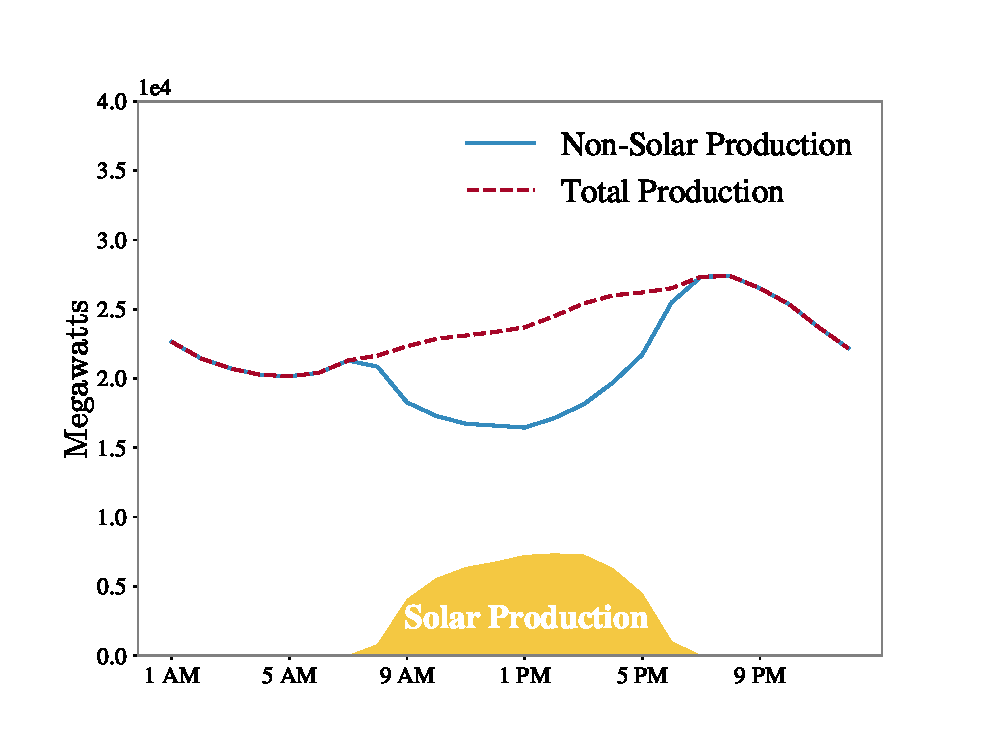
\includegraphics[width=13cm]{duck_curve.eps}
    \caption{Energy production in California on October 22, 2016.\cite{caiso} Total production is lowest in the early hours of the morning and peaks in the evening. Solar production peaks in the middle of the day.}
    \label{fig:duck_curve}
\end{figure}
Of all the previously discussed energy extraction technologies, solar has the fewest issues, after all, its hard to complain about free energy raining from the sky---in fact, most of the work since 1905 has been in designing the best bucket to capture it in. However, solar does have its foibles. Apart from solar's obvious and most nefarious enemy, the cloud, much of solar's issues lie in its interface with the existing electrical grid and its relatively low energy density. Since solar does not produce energy during the night, conventional fossil fuel plants need to pick up the slack. In the presence of solar power, these base load providers see a large dip in demand during the day (Fig. \ref{fig:duck_curve}), the time when solar is providing a significant portion of the electricity. Peak electricity usage ramps up in the late afternoon and peaks in the evening hours, precisely when solar production is decreasing. This means the base load providers have to quickly ramp up from a very low production level to a very high production level. This is not always possible and this problem only gets worse with more solar panels connected to the grid. Additionally, most base load providers are only economical if they produce a certain amount of electricity 24/7. If solar provides more electricity than the grid can handle, service managers would have to shutoff some of the panels to avoid damaging the grid; wasting electricity. This problem is exacerbated by the highly distributed nature of solar---solar requires a large collection area and, since there are few large open fields near major population centers, many smaller solar installations are installed. While most of these issues could be resolved with a better designed electrical grid, the fact remains that solar doesn't work at night and fossil fuel burning base load providers have to be utilized. Solar only solves the problem during the day. To solve the problem during the night, we have to look towards a new technology. 

\section{Alternative Energy: Possible Future}
A good alternative energy power plant should not subject to the whims of the weather, be energy dense both in terms of the fuel and in terms of the power plant itself, location independent, and produce no long lasting harmful by-products, e.g. carbon dioxide and nuclear waste. These criteria precludes all of the previously discussed energy sources. Fortunately, there is an energy source in development that meets most of the criteria: nuclear fusion. Unlike nuclear fission, fusion fuel does not produce any long lasting radioactive waste nor does it produce carbon dioxide. There is also no possibility of a meltdown and it uses less fuel. It has all the benefits of fission without many of its problems.

\subsection{Nuclear Fusion}
In nuclear fission, larger nuclei are split, creating smaller nuclei. Fusion is the opposite process in which we take lighter nuclei and fuse them together to create heavier nuclei. In either process, energy is released. To understand where this energy comes from we must consider the nature of the nucleus, particularly how the protons and neutrons are held together. There are two opposing forces at play in a nucleus: the strong force, which keeps the nucleus together, and electromagnetic force, which wants to tear the nucleus apart. This dance of forces means that every nuclei has an internal energy level---a consequence of quantum mechanics.
We can represent this energy level using the binding energy of the nucleus (Fig. \ref{fig:binding_energy}). The binding energy is the work required to disassemble the nucleus. The \textit{larger} the binding energy, the \textit{lower} the nucleus's energy level. We can change the energy level of a nucleus by adding or removing nucleons---protons or neutrons. If the change results in an lower energy state, then the excess energy is released in the form of kinetic energy. The amount of energy released is given by the difference in the binding energy of the starting and ending nuclei. According to Figure \ref{fig:binding_energy}, there is only two ways to release energy from a nucleus: start with a heavy element and reduce its mass (fission) or start with a light element and increase its mass (fusion).
\begin{figure}[h!]
    \centering
    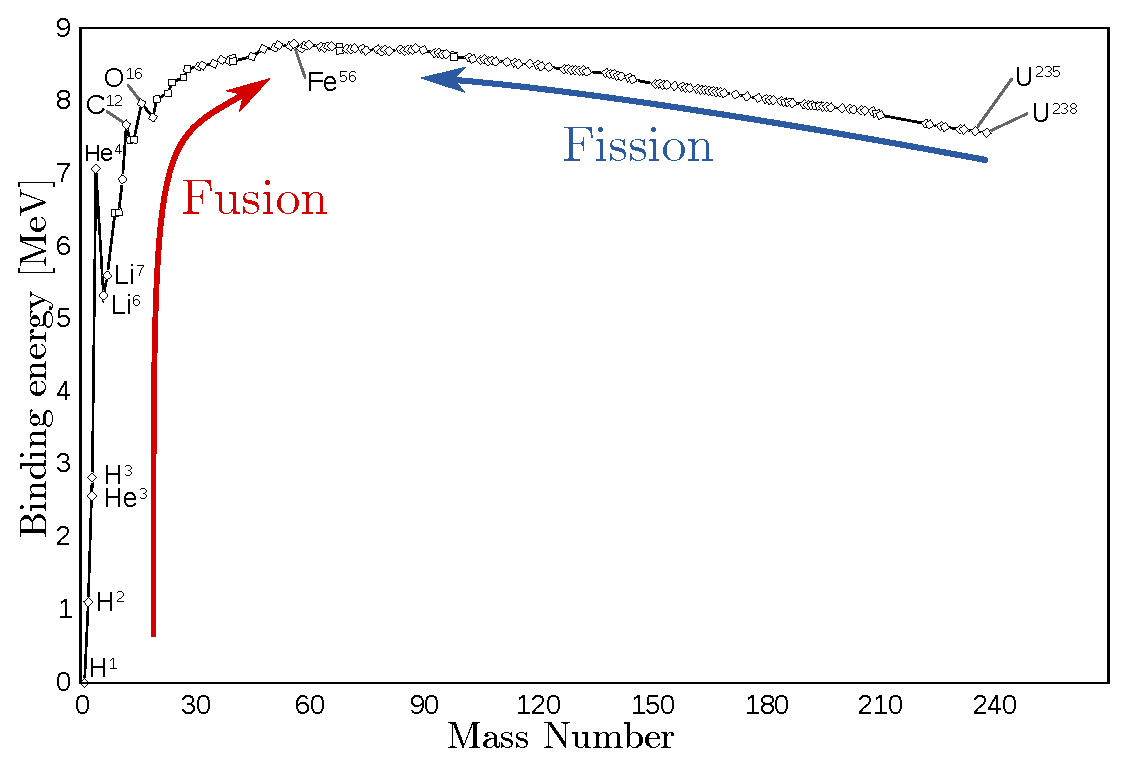
\includegraphics[width=13cm]{annotated_binding_energy.eps}
    \caption{Binding energy of nuclei. A change in the binding energy releases kinetic energy.}
    \label{fig:binding_energy}
\end{figure}

As can be seen in Figure \ref{fig:binding_energy}, fusion releases much more energy than fission per nucleon added. So what lighter elements should we fuse? Before we answer that, there are a few things we must consider: the energy needed to fuse, which we want to minimize; the output energy, which we want to maximize; and the cross section or probability of the interaction, which we also want to maximize. With these three criteria in mind, there are three particularly attractive candidate fuels: Deuterium--Tritium (D-T), Deuterium--Deuterium(D-D), and Deuterium--He$^3$(D-He$^3$). Table \ref{tab:fuel} shows the possible fuels and their properties.
\begin{table}[ht]
    \centering
    \caption{Possible fusion fuels. Due to its relatively large cross section at expected burning temperature and energy gain D-T fuel is the most achievable option. However, the Coulomb scattering cross section is orders of magnitude larger than the fusion cross sections. Because of this, the fuel is much more likely to just bounce off each other than fuse.}
    \label{tab:fuel}
    \begin{tabular}{cccc}
        \textbf{Fuel} & \textbf{Exhaust} & \textbf{Energy Gain} & \textbf{Cross Section @ 15 keV} \\ \hline \hline 
        D + T & $\alpha$ + n & 17.6 MeV & $1.48 \times 10^{-1}$ b \\[5pt]
        D + D & \begin{tabular}[c]{@{}c@{}}T + p (50\%)\\ He$^3$ + n (50\%)\end{tabular} & 3.65 MeV & $1.18 \times 10^{-3}$ b \\[10pt]
        D + He$^3$ & $\alpha$ + p & 18.35 MeV & $7.94 \times 10^{-6}$ b \\[5pt] \hline
    \end{tabular}
\end{table}
Figure \ref{fig:scattering} shows the cross sections of the different fusion fuels as a function of energy. The D-T fusion cross section is consistently larger than the other fuels and this, coupled with the large energy gain, lends itself to be the fusion fuel of choice.

However, if fusion was just a matter of colliding the fuel together at high energy, we would of achieved fusion decades ago; after all, CERN routinely collides particles together at TeV energies---more than enough for fusion to occur. The issue is that the Coulomb scattering cross section is orders of magnitude larger than the fusion cross sections (Fig \ref{fig:scattering}). This means that it's much more likely that the fuel will bounce off each other than fuse. Its rather like playing pool without the bumpers. The probability of getting a ball in a pocket is rather small. It's much more likely the ball will fall off the table and go out of play. However, if we put the bumpers back on, the balls become confined and we have more opportunities for getting a ball in a pocket. Likewise, if we contain the fuel, it will have more chances to fuse.
\begin{figure}[ht]
    \centering
    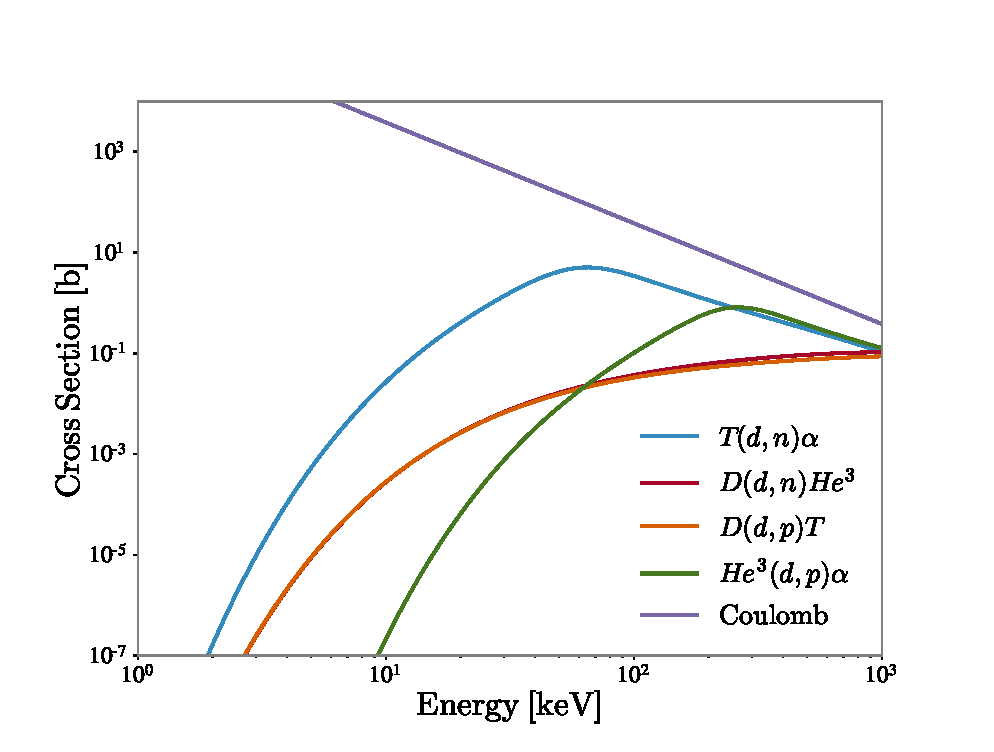
\includegraphics[width=13cm]{cross_sections.eps}
    \caption{Fusion and Coulomb scattering cross sections.}
    \label{fig:scattering}
\end{figure}
When contained and heated, the fuel becomes a plasma, a hot gas composed entirely of ions and electrons. Unlike other materials whose dynamics of motion are determined by forces between neighboring regions, the charge separation that exists in plasmas give rise to electromagnetic fields, which results in complex collective phenomena.

Designing a reactor that can effectively contain the plasma at the required temperatures is difficult and it is not yet clear that this can be done in a cost effective manner. Just having materials that can withstand a fusion environment is still an open area of research. Additionally, while the fuel itself does not produce any long lasting radioactive waste, it does produce high energy neutrons, which can irradiate reactor materials and compromise structural integrity. This leads to reactor components having a finite lifetime, after which the irradiated material needs to be stored, similar to fission. Fortunately, the amount of waste is considerably less than the amount produced by fission and has a shorter half-life. Fusion reactors also have more flexibility in regards to the materials used than fission reactors. This allows fusion reactors to use materials that are less susceptible to being irradiated. For instance, Vanadium is much less susceptible to being irradiated than stainless steel. However, research into the various Vanadium alloys for use in fusion reactors has been limited. 

The fusion fuel may also be a problem. While Deuterium is abundant, there is only a small amount of Tritium on earth. Tritium can be made by bombarding Lithium with high energy neutrons, but there is not yet an infrastructure in place for large scale production. It has been suggested that a Lithium breeder blanket can protect the outer materials from the neutron flux, provide a way of extracting energy, and produce the Tritium needed, but the feasibility of such a design has not yet been demonstrated.

\begin{figure}
    \centering
    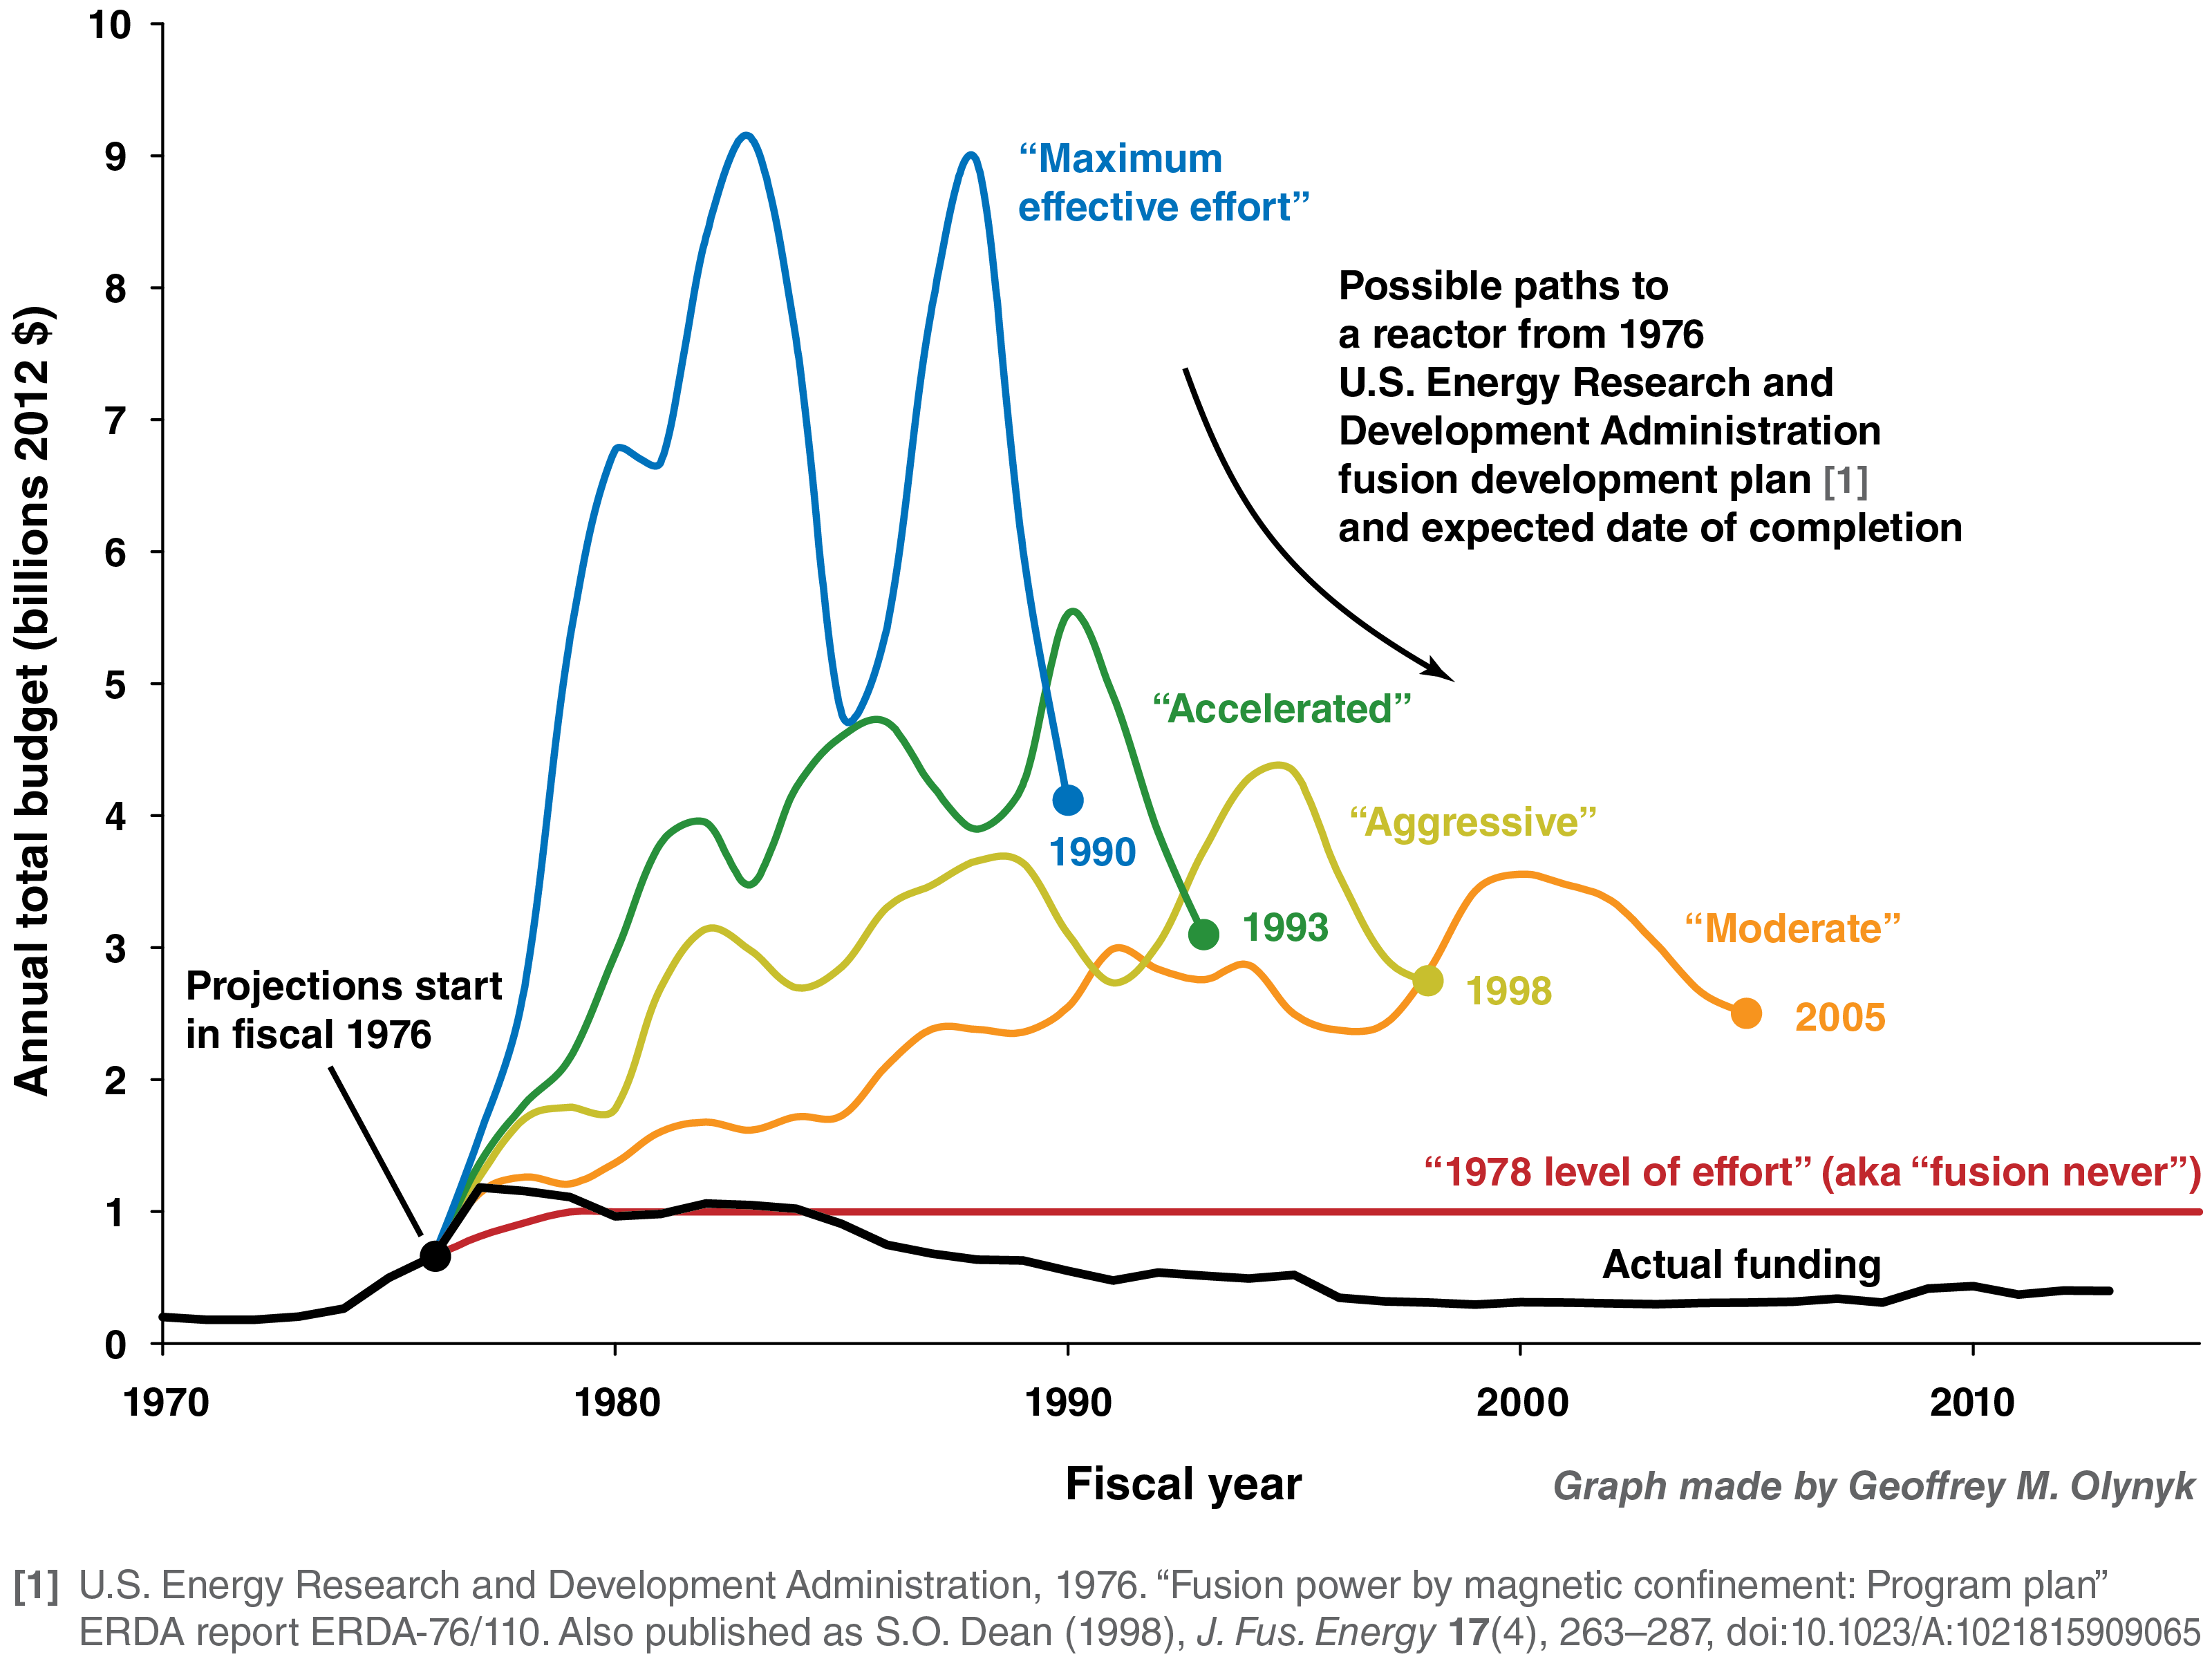
\includegraphics[width=12cm]{figures/fusion_never.png}
    \caption{Graph of U.S government magnetic fusion research budget compared to 5 funding scenarios from the 1976 Energy Research and Development Administration development plan.\cite{1976_fusion}}
    \label{fig:fusion_never}
\end{figure}
The aforementioned issues are not insurmountable; however, progress towards solving them is heavily dependent on the availability of funding. Unfortunately, fusion research has been chronically underfunded for decades. Since its inception in 1955, the U.S. fusion program has, adjusted for inflation, spent total of 42.6 billion\footnote{This figure includes both the budget for the magnetic and inertial confinement programs} dollars. To put this into perspective, NASA's 2018 budget was 20.7 billion dollars--just under half of the total amount spent on the fusion program over its entire 63 year history. Some may argue that we have spent too much on fusion research, but the reality is that we have spent too little. Figure \ref{fig:fusion_never} shows a graph of the budget for the U.S. Magnetic Fusion Energy program compared against five funding scenarios\cite{1976_fusion}. At the current levels of funding, there is a very real possibility that fusion energy will never exist---a hard truth that many young fusion scientists need to accept.
However, just because something is difficult doesn't mean its not worth doing. The benefits of fusion far outweigh its costs.

\subsection{Tokamaks}
\begin{figure}[ht]
    \centering
    \includegraphics[width=13cm]{tokamak.eps}
    \caption{Toroidal magnetic configuration of a tokamak. The toroidal field is provided by a series of field coils and the poloidal field is primarily generated by an electric current with a set of poloidal coils to assist with shaping. This fields give rise to a helical magnetic field which is necessary to maintain pressure balance. Figure modified from original\cite{geiger2013thesis}.}
    \label{fig:tokamak}
\end{figure}
In the 60+ years of fusion research, there have many different confinement schemes that have been tried. The most promising is the Tokamak.

Invented in the 1950's by Soviet physicists, the tokamak uses magnetic fields in a toroidal configuration to confine the plasma (Fig. \ref{fig:tokamak}). The principal toroidal magnetic field is provided by a series of field coils. In order to balance the plasma pressure, a current is run through the plasma to generate a poloidal field---additional poloidal field coils are also used for plasma shaping. The combination of the toroidal and poloidal field give rise to a helical magnetic field.

After an initial false start of disseminating their results in 1965, by 1969 the Soviet physicists had demonstrated that the tokamak outperformed all previous confinement schemes. A flood of small tokamaks were built in the following few decades. However, research showed that larger devices better contained the plasma and, as a result, many of the small tokamaks were decommissioned in favor of larger tokamaks. In the following sections, we will briefly discuss three of these larger tokamaks: DIII-D, ASDEX Upgrade, and NSTX-U.

\subsubsection{DIII-D}
\begin{figure}[ht]
    \centering
    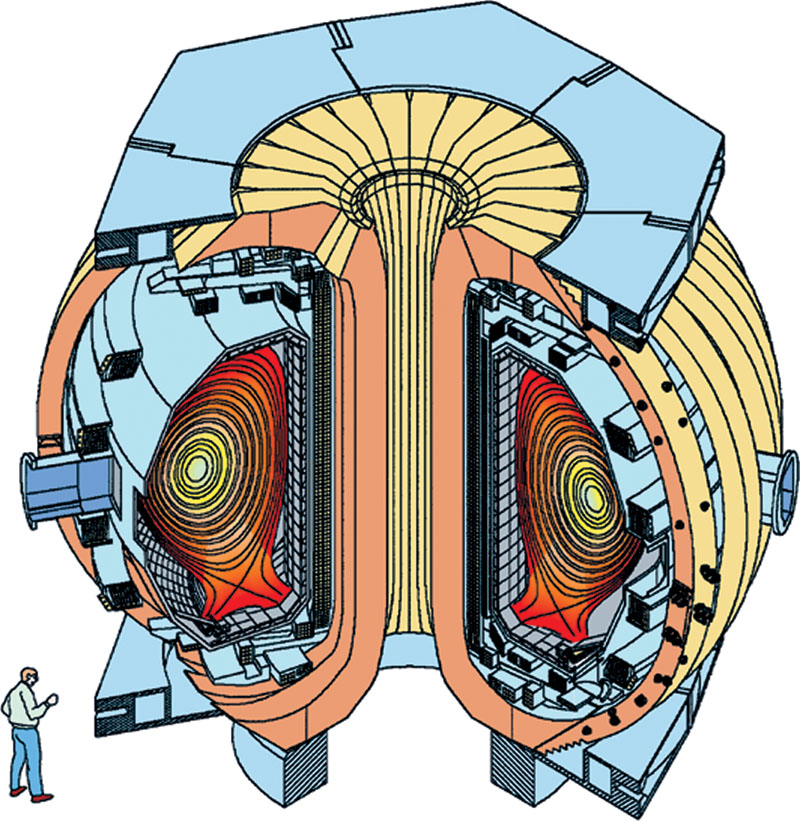
\includegraphics[width=10cm]{DIII-D.jpg}
    \caption{DIII-D Tokamak}
    \label{fig:d3d}
\end{figure}
Located at General Atomics in San Diego, CA, the DIII-D tokamak(Fig. \ref{fig:d3d}) is currently the largest operating tokamak in the United States\cite{luxon2002design}.
Originating out of the Doublet III experiment, the DIII-D tokamak began operations in 1986. DIII-D is known for it advanced shaping capabilities, which allows it to achieve high plasma $\beta$\footnote{plasma $\beta$ is the ratio of the plasma pressure to the magnetic pressure} with a lower magnetic field. The plasma heated with 8 neutral beam injection (NBI) systems, which can provide up to 20 MW of heating. Additional heating is done via radio frequency (RF) injection in the forms of ion cyclotron resonance heating (ICRH) and electron cyclotron resonance heating (ECRH). DIII-D's operating parameters are given in Table \ref{tab:d3d}.
\begin{table}[h!]
    \centering
    \caption{DIII-D Operating Parameters\cite{luxon2002design}.}
    \label{tab:d3d}
    \begin{tabular}{ccccc}
        \textbf{Minor Radius} & \textbf{Major Radius} & \textbf{Magnetic Field} & \textbf{Heating} & \textbf{Current} \\ \hline \hline
        0.67 m & 1.67 m & 2.2 T & 23 MW & 2 MA \\ \hline
    \end{tabular}
\end{table}

\subsubsection{ASDEX Upgrade}
\begin{figure}[ht]
    \centering
    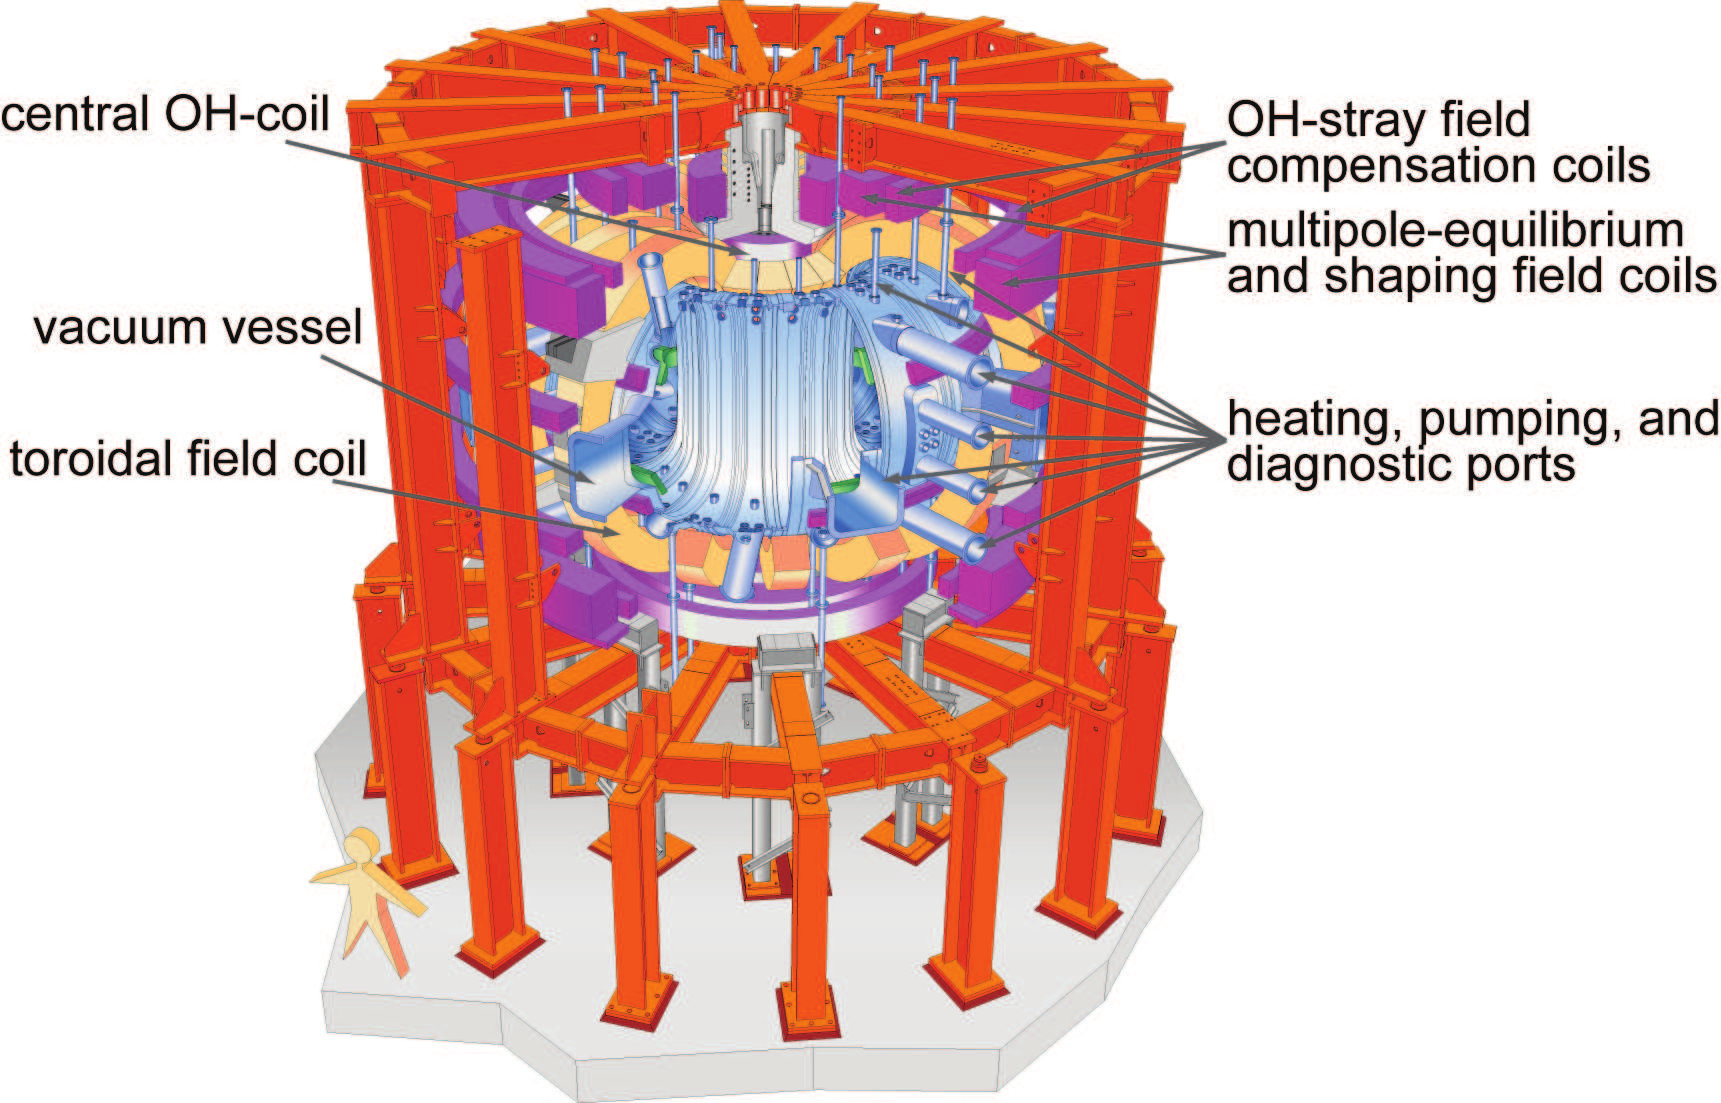
\includegraphics[width=12cm]{asdex.jpg}
    \caption{ASDEX Upgrade Tokamak\cite{geiger2013thesis}}
    \label{fig:augd}
\end{figure}
Beginning operation in 1991, ASDEX Upgrade(Fig. \ref{fig:augd}) is the successor to the successful \textbf{A}xially \textbf{S}ymmetric \textbf{D}ivertor \textbf{Ex}periment (ASDEX) which discovered the High-confinement operating mode (H-mode)\cite{wagner1982hmode}. It is currently the third largest fusion device in Europe, behind the Wendelstein 7-X stellarator\cite{wendelstein7x1993} and Joint European Torus (JET)\cite{jet1985}. It is comparable to the DIII-D tokamak. Up to 33 MW of heating power is provided by 4 NBI systems, ICRH, and ECRH. ASDEX Upgrade's operating parameters are given in Table \ref{tab:augd}. 
\begin{table}[]
    \centering
    \caption{ASDEX Upgrade Operating Parameters}
    \label{tab:augd}
    \begin{tabular}{ccccc}
        \textbf{Minor Radius} & \textbf{Major Radius} & \textbf{Magnetic Field} & \textbf{Heating} & \textbf{Current} \\ \hline \hline
        0.5 m & 1.65 m & 2.5 T & 33 MW & 1.4 MA \\ \hline
    \end{tabular}
\end{table}

\subsubsection{NSTX \& NSTX-U}
\begin{figure}[ht]
    \centering
    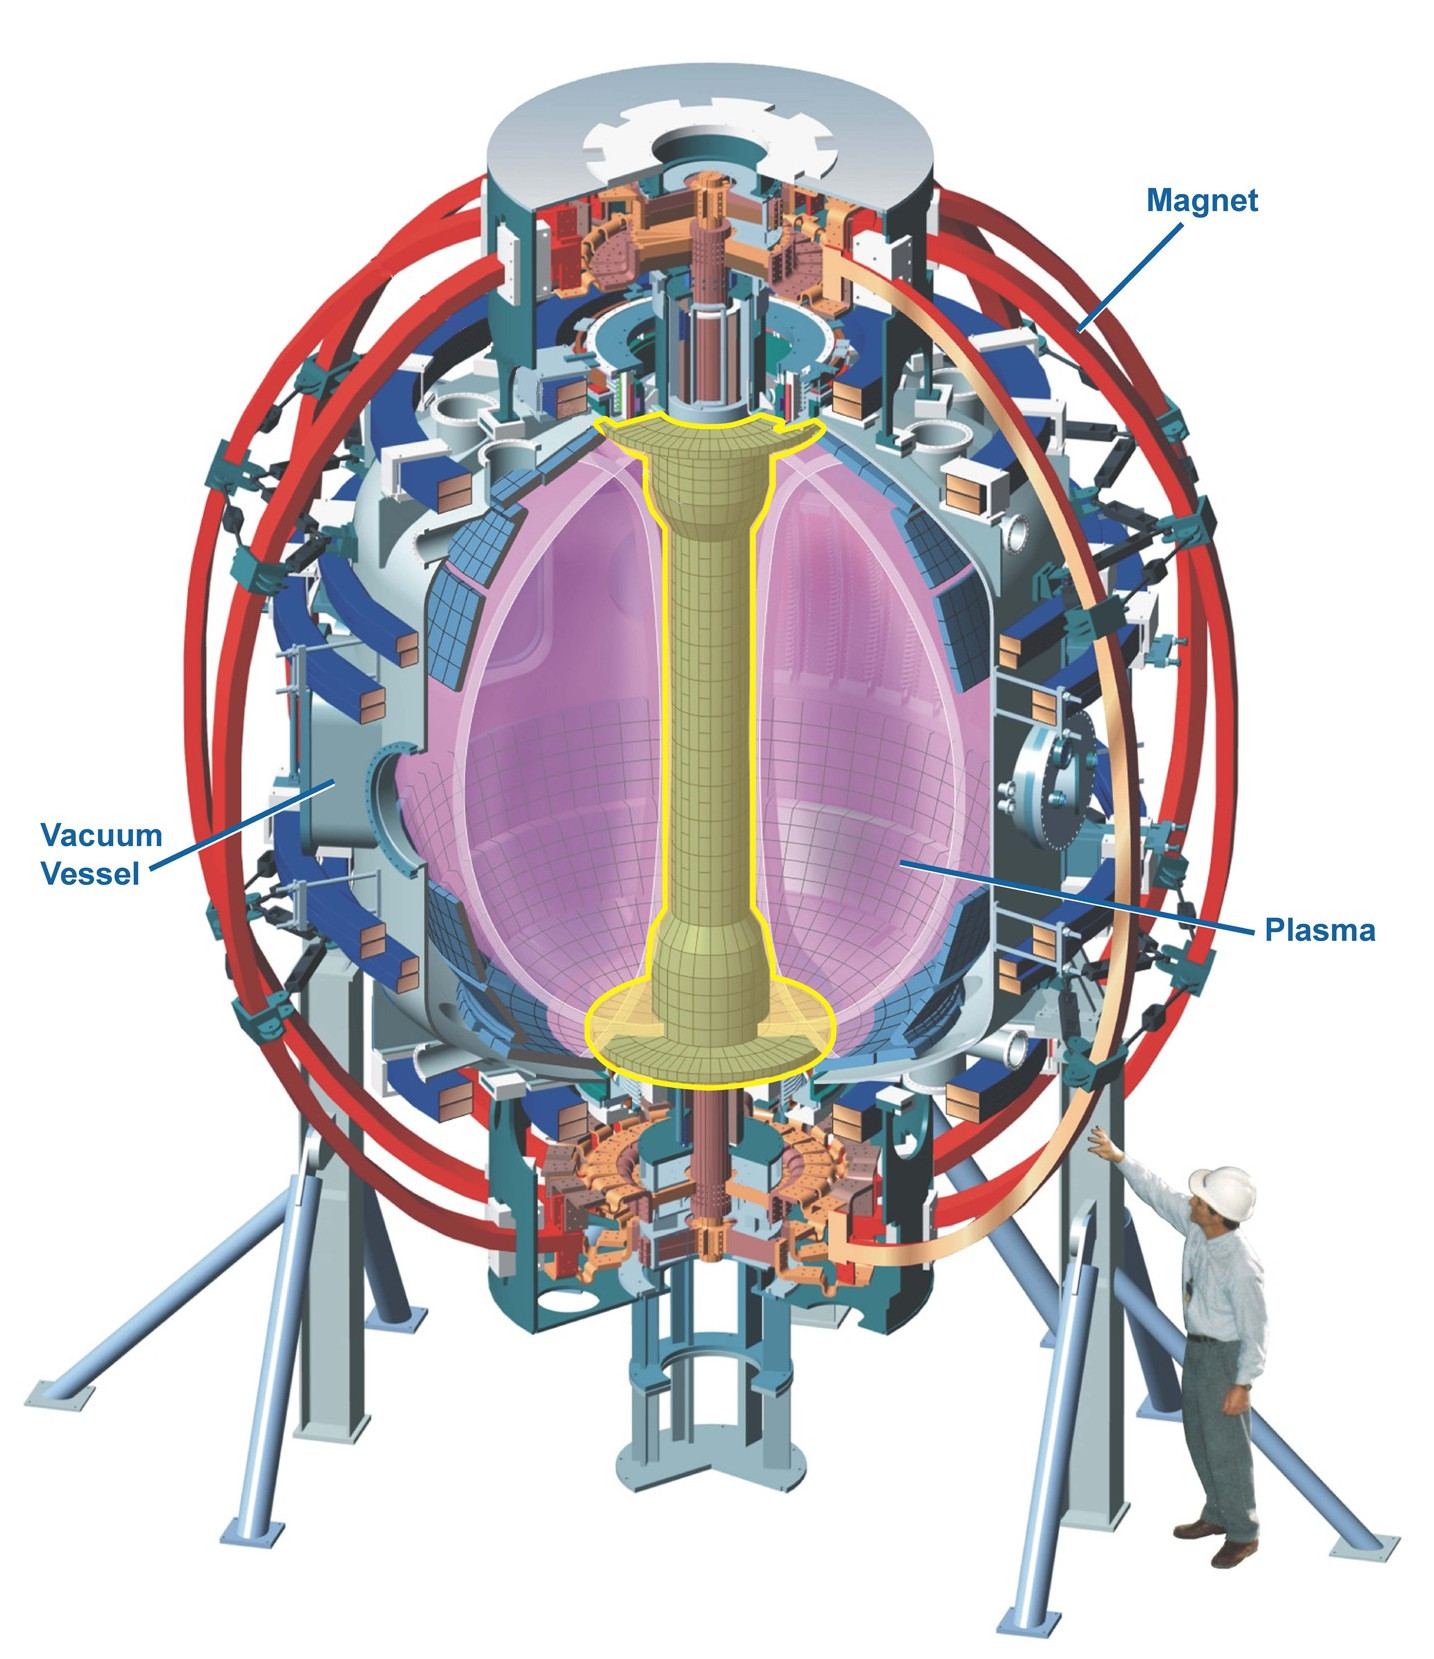
\includegraphics[width=10cm]{nstxu.jpg}
    \caption{NSTX-U Spherical Tokamak}
    \label{fig:nstx}
\end{figure}
Unlike the previous tokamaks, NSTX and its recent upgrade, NSTX-U, is a spherical tokamak. Spherical tokamaks have a much smaller aspect ratio: $R/a\sim1$ as opposed to $R/a\sim3-4$ in conventional tokamaks. A small aspect ratio allows spherical tokamaks to easily achieve high plasma $\beta$ with a low magnetic field. This could lead to smaller and more economical fusion reactors. NSTX began operation in 1999 and was upgraded in 2015. It is heated by NBI and ICRH. NSTX-U's operating parameters are given in Table \ref{tab:nstx}. 
\begin{table}[h!]
    \centering
    \caption{NSTX/NSTX-U Operating Parameters}
    \label{tab:nstx}
    \begin{tabular}{ccccc}
        \textbf{Minor Radius} & \textbf{Major Radius} & \textbf{Magnetic Field} & \textbf{Heating} & \textbf{Current} \\ \hline \hline
        0.68 m & 0.85 m & 0.3 T & 11 MW & 1.4 MA \\ \hline
    \end{tabular}
\end{table}

\subsection{The Lawson Criterion and Fast ion Confinement}
In order to maintain steady-state operation in the aforementioned tokamaks, the power going into the system must equal the power going out. There are several power sources in a tokamak. The power supplied by fusion, $P_{fusion}$, is broken up among its exhaust. For D-T fuel only the power from the alpha particles, $P_\alpha$, contributes to the power balance as the neutrons, having no charge, do not interact with the magnetic field and their power is deposited into the vessel wall or, in the case of a reactor, the blanket. Due to poor confinement and radiative emission, there is also lost power, $P_{lost}$. Additionally, if the power supplied by the fusion products is insufficient to keep the plasma going, external power, $P_{ex}$, must be supplied---usually in the form of NBI, ICRH, and ECRH. The power balance equation is then
\begin{equation}\label{eq:power_balance}
    \frac{dW}{dt} = P_\alpha + P_{ex} - P_{lost} = 0
\end{equation}
where $W$ is the energy density.

From this equation, we can extract a few useful concepts. In steady-state, the time it takes a plasma to dump all its energy, the energy confinement time, is given by
\begin{equation}\label{eq:tau_e}
    \tau_E = \frac{W}{P_{lost}}.
\end{equation}
From the power balance equation, we can also define the amplification factor, $Q$, which is the ratio of the fusion power and the external power: $Q = P_{fusion}/P_{ex}$. A $Q > 1$ is a minimum requirement in a fusion reactor, otherwise, more energy is put in than is generated. Most importantly, ignition---the point where the alpha heating is large enough to compensate for any losses---occurs when $P_\alpha > P_{lost}$. If the plasma ignites, it becomes self sustaining and external heating can be shut off---known as the burning plasma regime; a desirable quality in a reactor.
In order to ignite, the plasma has to be dense enough, hot enough, and confined for a long enough time. These conditions are codified in the Lawson Criterion---also derived from the energy balance equation---which can take the form of a triple product,
\begin{equation}\label{eq:lawson}
    nT\tau_E > \frac{12}{\langle \sigma v \rangle} \frac{T}{\mathcal{E}_\alpha} > 3\times10^{21} \; \rm{m^{-3}\, keV\, s}, \quad \rm{for\;D-T\;fusion}.
\end{equation}
There are many ways this criterion could be met, for example by having $n = 10^{20}\, \rm{m^{-3}}$, $T = 10\,\rm{keV}$, and $\tau_E = 3\,\rm{s}$.

To get into the burning plasma regime, one must first apply enough external heating to reach the ignition point. This is usually done through a combination of neutral beam injection and RF heating. This heating creates a small population of ions whose temperature is much greater than the background plasma. These fast ions start out at a high energy ($\sim 80$ keV) and through a series of collisions with the background plasma, thermalize. The process of thermalization transfers energy to the background plasma, increasing its temperature. The fast ions, while necessary to heat the plasma, bring with them a series of problems that need to be overcome in order to achieve fusion.

One of the main problems that fast ions bring is their ability to resonate with a class of instabilities called Alfv\'en eigenmodes\cite{heidbrink2008basic}. The fast ions that are resonant with the mode can either take energy away from the mode, making the plasma more stable and enhancing confinement, or, more commonly, they drive the instability, making the plasma more unstable and degrading confinement. In the presence of many Alfv\'en eigenmodes, fast ions are redistributed into regions where they are lost, either to the wall or through charge exchange with edge cold neutrals that exist in the outer layers of the tokamak. As a result, the fast ions transfer less energy to the thermal ions, which affects heating and also global confinement.\cite{heidbrink2014confinement,holcomb2015fast}

The fast-ion resonances occur in very particular regions in phase-space. In order to understand the wave-particle interactions, we need to know where the fast ions are relative to these resonances. This information is encoded in the fast-ion distribution function. Knowing the form of the fast-ion distribution function is the key to understanding not only wave-particle interactions but all of fast-ion physics.

The goal of this thesis is to infer the fast-ion distribution function from experimental measurements. The outline of the thesis is as follows. In Chapter \ref{chap:diagnostics}, we go over a few of the diagnostics that are sensitive to the fast ions. We discuss, in detail, how they encode information about the fast-ion distribution and how this information is translated via the diagnostics forward models into measurable quantities. In Chapter \ref{chap:fidasim}, we discuss the development of FIDASIM\cite{heidbrink2011code,geiger2013thesis,FIDASIM}, the practical implementation of the forward models discussed in Chapter \ref{chap:diagnostics}. In Chapter \ref{chap:weights}, we discuss and derive diagnostic velocity-space weight functions, which are used to interpret diagnostic signals.\cite{heidbrink2007,salewski2011,salewski2012,Muscatello2012,collins2015characterizing,collins2016observation,collins2017phase,collins2016critical,heidbrink2016interpretation} This chapter also introduces orbit weight functions\cite{stagner2017action}, which can be used to linearize diagnostic forward models without loss of accuracy. In Chapter \ref{chap:velocity-space_tomography}, we benchmark\cite{jacobsen_stagner2016} inference methods used in Velocity-space Tomography, a technique that uses the velocity-space weight functions to infer a local approximation of the fast-ion distribution function from experimental measurements.\cite{heidbrink2007,salewski2011,salewski2012,Muscatello2012,Salewski2014a,jacobsen2015,salewski2013_tomography,salewski2014_tomography,salewski2016,salewski2016high,weiland2016}
Chapter \ref{chap:orbit_tomography} introduces Orbit Tomography, an extension of Velocity-space Tomography that uses orbit weight functions to infer the entire fast-ion distribution function from experimental measurements. Orbit Tomography is used to infer a classically described DIII-D discharge and to study the redistribution of fast ions by a sawtooth crash in ASDEX Upgrade. Chapter \ref{chap:outlook} discusses future improvements and a possible application of Orbit Tomography to infer the runaway electron distribution function.

%%% Local Variables: ***
%%% mode: latex ***
%%% TeX-master: "thesis.tex" ***
%%% End: ***

\chapter{Fast-ion Diagnostics}\label{chap:diagnostics}
There is basically two ways diagnostics can probe the fast-ion distribution. The first is to directly collect samples from the distribution. Direct sampling of the distribution is difficult because any probe inserted into the plasma would not survive due to the highly corrosive environment of a fusion plasma. Because of this, samples can only be drawn from the very edge of the plasma where the environment is more friendly to diagnostics. This effectively limits the types of fast ions detected. Case in point, one of the few direct fast-ion diagnostics, the fast-ion loss detector (FILD), only measures---as the name suggests---fast-ions that are lost to the wall---a useful diagnostic but limited in the information gained about the fast-ion distribution as a whole.

A different approach to fast-ion diagnostics is to measure the byproducts of their interactions with the plasma. This approach allows for more information about the fast-ion distribution to be gained. The increased information, however, comes at a cost. Since the diagnostics do not directly measure the fast ions we must model what the detector would see for any given fast-ion---we call this the diagnostic's forward model. Even though we have more information about the fast-ion distribution it is garbled by the diagnostic's forward model. This makes the analysis of our data difficult. In experiment, we only ever see the noisy output of the forward model. In order to validate a theoretical model, we have to run the model through the diagnostic's forward model to get an apples to apples comparison with data. This is not an ideal scenario. Fortunately, as we will see in Chapter \ref{chap:tomography}, it is possible to reverse this process to obtain the fast-ion distribution from measurement alone. In order to do this we need the forward model of our diagnostics.

In the following sections we will discuss three different fast-ion diagnostics and their forward models: Neutral Particle Analyzers (NPA), Fast-ion D-$\alpha$ spectroscopy (FIDA), and neutron scintillators.

\section{Neutral Particle Analyzers}
\begin{figure}[ht]
    \centering
    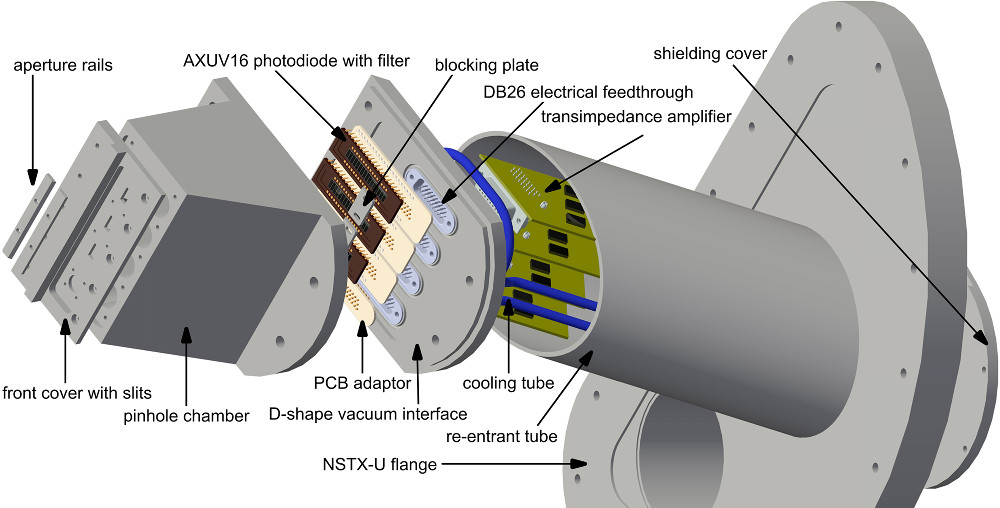
\includegraphics[width=12cm]{figures/nstx_npa.jpeg}
    \caption{Expanded view of NSTX-U's solid state neutral particle analyzer array.\cite{liu2014design}}
    \label{fig:npa}
\end{figure}
Neutral particle analyzers detect fast ions that have undergone a charge exchange (CX) reaction with a neutral population within the plasma, becoming a fast neutral. Since the fast neutral is not confined by the magnetic field, information about the fast ions at the center of the plasma can be attained. Neutral particle analyzers are one of the first fast-ion diagnostics\cite{artsimovich1969experiments}. However, in recent years there has been a bit of a renaissance in their design. Compact solid state analyzers\cite{zhu2012compact} allowed for more sightlines in a smaller space. This type of design has recently been installed on NSTX-U (Fig. \ref{fig:npa}). Most recently, an Imaging NPA that combines the best aspects of traditional analyzers and fast-ion loss detectors has been deployed at DIII-D and has shown excellent initial results\cite{du2018inpa}.

\subsection{Forward Model of the Neutral Particle Analyzer}
As mentioned, neutral particle analyzers detect fast neutrals that are born of charge exchange reactions with the neutral populations within the tokamak, in which there are several.
Neutral beam injection creates three distinct neutral populations due to the acceleration of molecular hydrogen.
During the neutralization phase of neutral beam injection the molecular forms are eliminated and the gained energy is split evenly among the atoms.
The energy of each population is given by $E_i = E_1/i$ where $i$ is the number of hydrogen atoms in each molecule.
The velocity distribution of each species is tightly focused and can be approximated by a Dirac delta function.
A fourth population of neutrals forms when injected neutrals charge exchange with thermal ions creating a thermal ``halo'' with a shifted Maxwellian velocity distribution. A fifth type of neutral occur when thermal ions reach the cold edge of the plasma and neutralize. This creates a cold edge neutral population that has a shifted Maxwellian velocity distribution. These cold edge neutrals are always present and are independent of the neutral beam. Since certain signals are only present when the neutral beam is on we tend to separate the signals that come from CX with the beam (active signals) and signals that originate from CX with the cold edge neutrals (passive signals) though the following derivation of the forward model makes no such distinction.

Consider a beam of fast ions traveling through a cloud of neutral particles. The fast ions can undergo the following charge exchange reaction to create a fast neutral
\begin{equation}
    H_f^+ + H(m) \rightarrow H_f(n) + H^+\,,
\end{equation}
where $H_f^+$ is the fast ion, $H(m)$ is the donor neutral in energy state $m$, $H_f(n)$ is the fast neutral in energy state $n$, and $H^+$ is the newly created ion.
The rate in which the fast ion, when interacting with the $k$ different neutral populations, produces a fast neutral in a given energy level is given by
\begin{equation}\label{eq:cx_rates}
    \mathbf{f}(t=0) = \sum_k \left [ \int \mathbf{X}(\mathbf{v}_f - \mathbf{v}) \cdot \mathbf{d}_k\, ||\mathbf{v}_f - \mathbf{v}||\, f_k(\mathbf{v})\, d\mathbf{v} \right ]
\end{equation}
where $\mathbf{X}$ $[cm^2]$ is a $n \times m$ matrix of the charge exchange cross sections, $\mathbf{d}_k$ $[cm^{-3}]$ is the densities vector of the $m$ energy levels of the donor neutral, and $f_k$ is the velocity distribution of the $k^{th}$ neutral population. This is called the neutral population flux.
The neutral population flux, $\mathbf{f}$, evolves in time as it travels through the background plasma due to collisions with the different plasma species, the most significant collisions being:
\begin{itemize}
    \item excitation and/or ionization with electrons,
    \item excitation and/or ionization with ions,
    \item charge exchange with ions.
\end{itemize}

The effects of the different collisional processes on the population flux can be modeled by the following matrix differential equation. 
\begin{equation}\label{eq:colrad}
    \frac{d \mathbf{f}}{dt} = \mathbf{C} \cdot \mathbf{f}
\end{equation}
where $\mathbf{C}$ is a matrix of the rate coefficients for the collisional and atomic transitions.
The full derivation of Eq. \ref{eq:colrad} is given in Appendix \ref{app:colrad}.

The solution of Eq. \ref{eq:colrad} takes the form of a matrix exponential
\begin{equation} \label{eq:neutral_flux}
    \mathbf{f}(t) = e^{\mathbf{C} t} \cdot \mathbf{f}(t=0) = \mathbf{S} \cdot e^{\mathbf{\Lambda} t} \cdot \mathbf{S}^{-1} \cdot \mathbf{f}(0)
\end{equation}
where $\mathbf{f}(t)$ is a vector of the neutral population flux [1/s] at time $t$, $\mathbf{S}$ is the matrix of the eigenvectors of $\mathbf{C}$ and $\mathbf{\Lambda}$ is a diagonal matrix containing the eigenvalues of $\mathbf{C}$.
Equation \ref{eq:colrad} depends on the local plasma parameters and is solved iteratively along the trajectory of the neutral. Figure \ref{fig:f_evolution} shows the evolution of the neutral population fluxes for two initial states: $f_1 = 1.0$ and $f_3=1$ with all other level populations set to zero. Despite the different initial conditions, the population fluxes trend toward an equilibrium. The time it takes to equilibrate depends on the initial states and the plasma parameters: the $f_1=1$ case equilibrates quickly and the $f_3=1$ case slowly. In experiment the $f_1$ level is the most populated so we expect the evolution of the population flux to be closer the $f_1=1$ case.
\begin{figure}[ht]
    \centering
    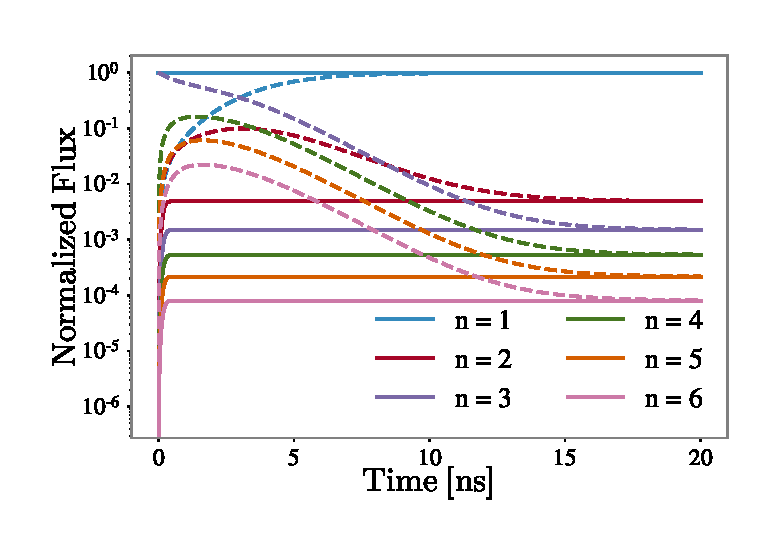
\includegraphics[width=10cm]{figures/f_evolution.eps}
    \caption{Evolution of the neutral population fluxes for two different initial conditions: $f_1=1$ (solid lines) and $f_3=1$ (dashed lines). Plasma parameters are held constant over time: $n_e = 6\times10^{13}\;cm^{-3}$, $T_e=T_i = 2\;keV$, and $Z_{eff} = 1.5$. At each time the fluxes are normalized such that $\sum_i f_i = 1$.}
    \label{fig:f_evolution}
\end{figure}

Should the trajectory of the neutral particle enter the detector the expected NPA signal for a fast ion with coordinates, $\mathbf{x}$, is then given by
\begin{equation}\label{eq:npa_weight}
    S_{NPA}(\mathbf{x}) = \epsilon(E) \sum_n \mathbf{f}(t_{det})
\end{equation}
where $t_{det}$ is the travel time to the detector and $\epsilon(E)$ is an energy dependent detector efficiency.

\section{Fast-ion D-$\alpha$ Spectroscopy}
\begin{figure}[ht]
    \centering
    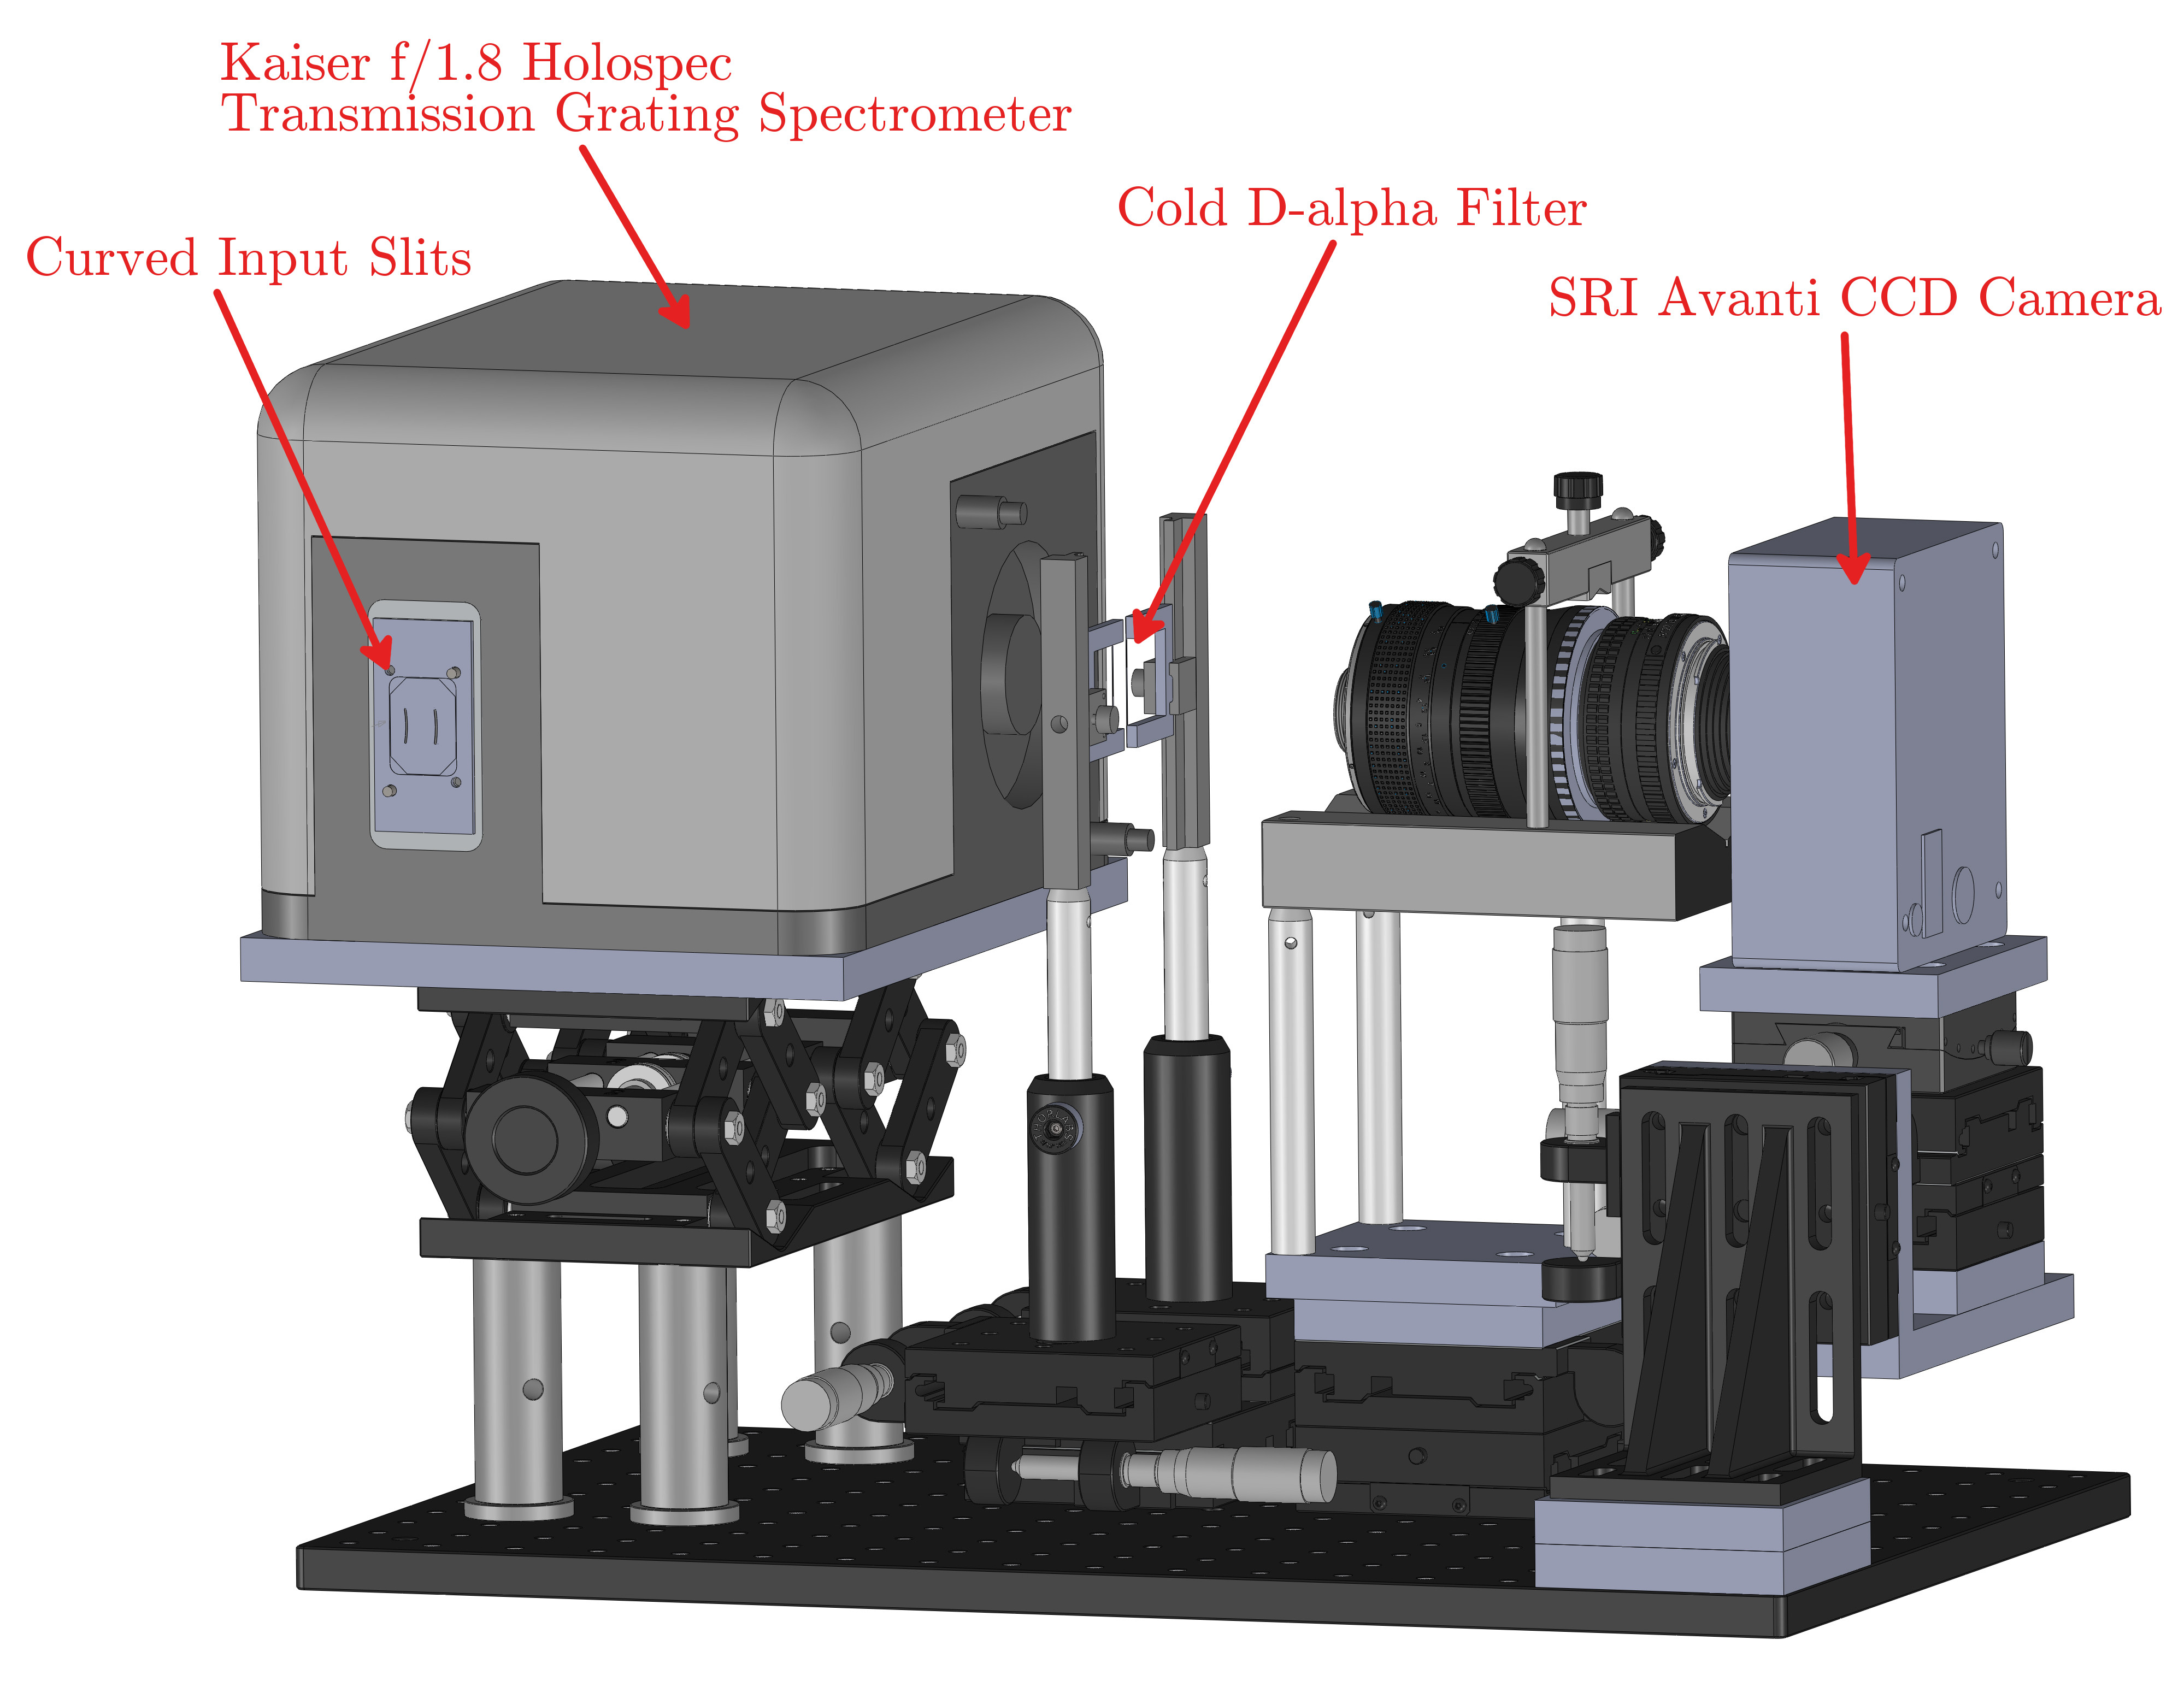
\includegraphics[width=12cm]{figures/d3d_fida.jpg}
    \caption{DIII-D's FIDA spectrometer\cite{muscatello2010}. Photons from the vessel travel through 33 optical fibers, 8 of which enter the spectrometer via input slits. The number of lines-of-sight are limited by the amount of available space on the CCD chip. To prevent saturation of the camera, the cold D-$\alpha$ emission is attenuated by a filter. Figure courtesy of Cami Collins}
    \label{fig:fida}
\end{figure}
Like the NPA diagnostic, charge exchange with a neutral population forms the basis for the Fast-ion D-$\alpha$ (FIDA) diagnostic\cite{heidbrink2004fida}. Where the NPA diagnostic measured neutrals, the FIDA diagnostic measures photons. When the fast neutral is created it can be born in the excited $n=3$ state. As the fast neutral travels through the plasma it will relax into the lower $n=2$ state and emit a photon. The Doppler shift of the photon contains information about the fast ion before it was neutralized. Unlike the NPA diagnostic the bulk of the FIDA diagnostic (the spectrometer, filters, and camera) is stored away from the machine. Figure \ref{fig:fida} shows DIII-D's FIDA diagnostic which is kept in a separate room from the machine; fiber optic lines carry the emitted light from the vessel to the spectrometer. In addition to detecting FIDA light, the diagnostic also detects thermal emission from the cold edge neutrals,neutral beam emission, and Oxygen V/Carbon II impurity emission. This complicates the design and analysis of the diagnostics. For instance, the line of sight geometry must be designed to cleanly separate the FIDA signal from the contaminating sources. Despite this complication, the FIDA diagnostic has become a standard fast-ion diagnostic with implementations at most major tokamaks\cite{heidbrink2010fast}.

\subsection{Forward Model of the Fast-ion D-$\alpha$ diagnostic}
After a fast-ion charges exchanges with a neutral---the physics of which is identical to the NPA diagnostic---the resultant fast neutral can be born in an excited state. As it travels the fast neutral will emit photons, the amount of which depends on the neutral population.
The neutral population after a time $t$, $\mathbf{n}(t)$, is found by integrating Eq. \ref{eq:neutral_flux},
\begin{equation}\label{eq:neutral_population}
    \mathbf{n}(t) = \mathbf{S} \cdot ( \mathbf{\Lambda}^{-1} \cdot e^{\mathbf{\Lambda} t} - \mathbf{\Lambda}^{-1} ) \cdot \mathbf{S}^{-1} \cdot \mathbf{f}(0).
\end{equation}
If $t$ represents the time spent inside a measurement volume, $V$, the Balmer-$\alpha$ photon flux is given by
\begin{equation}\label{eq:photon_flux}
    \Phi_\gamma = n_{3}(t)\,A_{3 \rightarrow 2}
\end{equation}
where $A_{3\rightarrow2}$ is the spontaneous emission rate for the D-$\alpha$ transition.
The photon radiance can then be calculated by integrating the photon flux density per steradian over the line of sight,
\begin{equation}\label{eq:photon_radiance}
    L_\gamma = \frac{1}{4\pi V} \int_{LOS} \Phi_\gamma\, dl .
\end{equation}

In the presence of a magnetic field, the motion of an ion will induce an electric field, breaking the spherical symmetry of the atom.
This allows for the existence of multiple stable states that have the same principle quantum number $n$.
This effect is called Motional Stark splitting.
It is simpler to use parabolic coordinates, $|k_1,k_2,m\rangle$, instead of the usual $|n,l,m\rangle$ spherical coordinates to solve for the perturbed energy levels of the Hydrogen atom. The parabolic coordinates are related to the spherical coordinates through the relation: $n = k_1 + k_2 + |m| + 1$.
For hydrogenic atoms the energy difference between the different stark states is proportional to the electric field strength and is given by
\begin{equation}\label{eq:stark_splitting}
    \Delta \mathcal{E}(n,k_1,k_2) = \frac{3\,n\,E\,a_0}{2}\,(k_1 - k_2) \quad [\mathrm{eV}]
\end{equation}
where $a_0$ is the Bohr radius and $E$ is the magnitude of the induced electric field\cite{bethe&salpeter}. Figure \ref{fig:stark_splitting} shows the splitting and the possible transitions for the $n=3\rightarrow2$ transition.
\begin{figure}[ht]
    \centering
    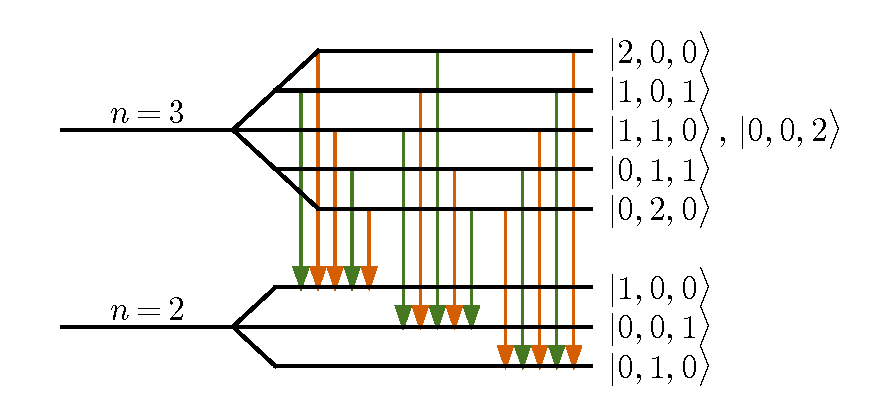
\includegraphics[width=10cm]{stark_splitting.eps}
    \caption{Stark splitting of the $n=3$ and $n=2$ energy levels of hydrogen. Higher levels indicate higher energy. States are labeled in parabolic coordinates $|k_1,k_2,|m|\rangle$. Possible transitions between states are indicated by arrows: green for $\sigma$ lines and orange for $\pi$ lines.}
    \label{fig:stark_splitting}
\end{figure}

As can be seen from Figure \ref{fig:stark_splitting}, the number of stark states for each principle quantum number is given by $2n-1$ and the transition from $n=3 \rightarrow 2$ creates 15 distinct spectral lines. The wavelength shift from the D-$\alpha$ line for the transition $|k_1,k_2,m\rangle \rightarrow |k_1',k_2',m'\rangle$ can be derived via the Taylor expansion of the Rydberg equation and is given by
\begin{equation}\label{eq:stark_lambda}
    \Delta \lambda(|k_1,k_2,m\rangle \rightarrow |k_1',k_2',m'\rangle) = \frac{3 \lambda_{0}^2\,a_0 (3(k_1-k_2) - 2(k_1' - k_2'))}{2hc} E \quad \rm{[nm]}
\end{equation}
where $\lambda_0$ is the unshifted wavelength (656.1 nm).
Taking into account the Doppler shift due to the line of sight geometry the wavelength for each Stark line is,
\begin{equation}\label{eq:wavelengths}
    \lambda(T) = \lambda_0 (1 + \Delta \lambda(T)/\lambda_0 + (\boldsymbol{\hat{\omega}} \cdot \mathbf{v}_f)/c),
\end{equation}
where $T =|k_1,k_2,m\rangle \rightarrow |k_1',k_2',m'\rangle$ and $\boldsymbol{\hat{\omega}}$ is a unit vector pointing toward the collection optics. The net effects of the Doppler and Stark shifts are shown in Figure \ref{fig:stark_doppler}.
\begin{figure}[ht]
    \centering
    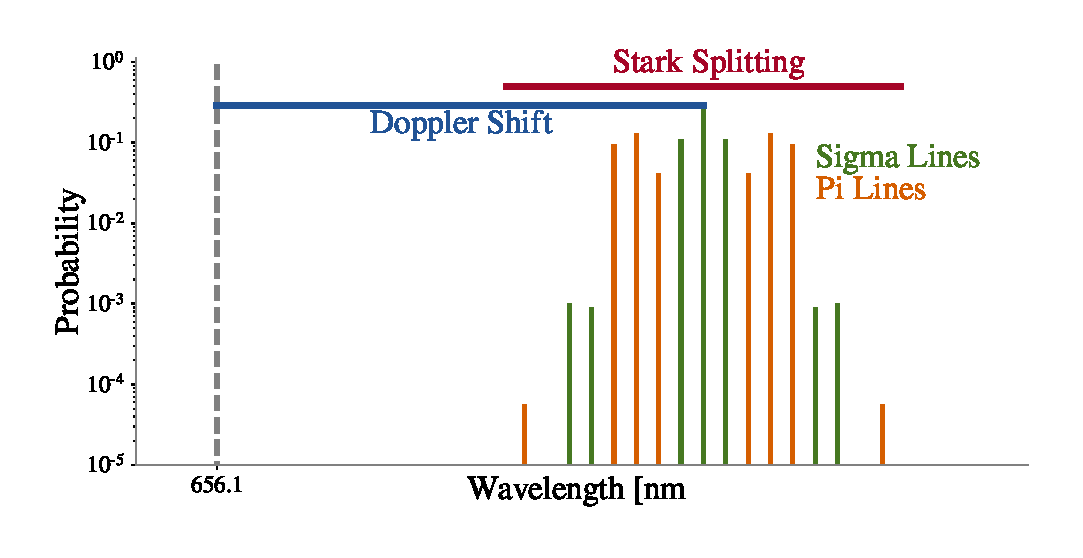
\includegraphics[width=10cm]{stark_doppler.eps}
    \caption{Doppler shift and Stark splitting on the D-$\alpha$ line. Stark line intensities are given in table \ref{tab:stark}.}
    \label{fig:stark_doppler}
\end{figure}

The photon radiance given in Eq. \ref{eq:photon_radiance} is distributed among the Stark lines.
The relative radiance of each Stark line is given by
\begin{equation}\label{eq:stark_intens}
I(T) = \epsilon(T) A(T)\,(1 \pm (\boldsymbol{\hat{\omega}} \cdot \mathbf{E})^2)
\end{equation}
where $A(T)$ is the probability of transition $T$ and $\epsilon(T)$ is the diagnostic efficiency of the transition. The relative probabilities for each transition is given in table \ref{tab:stark}. The expression in the parenthesis of Eq. \ref{eq:stark_intens} is the angular distribution of the emission which depends on the polarization of the transition: the plus sign for transitions that are linearly polarized \textit{perpendicular} to the electric field ($\sigma$ lines) and the minus sign for transitions that are linearly polarized \textit{parallel} to the electric field ($\pi$ lines).
Combining equations \ref{eq:photon_radiance}, \ref{eq:wavelengths}, and \ref{eq:stark_intens} gives the expected signal produced by a single fast ion with coordinates $\mathbf{x}$,
\begin{equation}\label{eq:fida_weight}
    S_{FIDA}(\lambda;\mathbf{x}) = \sum_T L_{\gamma}\, \frac{I(T)}{\sum_T I(T)} \delta(\lambda - \lambda(T)) \,.
\end{equation}
\begin{table}[ht]
\centering
\caption{Stark transitions and relative probabilities\cite{bethe&salpeter}. Transitions are given in parabolic coordinates. Degenerate initial states double the relative probability.}
\label{tab:stark}
\bgroup
\def\arraystretch{1.52}
\begin{tabular}{clr}
\textbf{Symbol} & \multicolumn{1}{c}{\textbf{Transition}} & \multicolumn{1}{c}{\textbf{$\mathbf{A_{rel}}$}} \\ \hline \hline
$\pi_{-7}$ & $|2,0,0\rangle \quad\! \rightarrow |0,1,0\rangle$ & $1$ \\
$\sigma_{-6}$ & $|2,0,0\rangle \quad\! \rightarrow |0,0,\pm1\rangle$ & $18$ \\
$\sigma_{-5}$ & $|1,0,\pm1\rangle \rightarrow |0,1,0\rangle$ & $2\times8$ \\
$\pi_{-4}$ & $|2,0,0\rangle\quad\! \rightarrow |1,0,0\rangle$ & $1681$ \\
$\pi_{-3}$ & $|1,0,\pm1\rangle \rightarrow |0,0,\pm1\rangle$ & $2\times1152$ \\
$\pi_{-2}$ & $|1,1,0\rangle \quad\!\rightarrow |0,1,0\rangle$ & $729$ \\
$\sigma_{-1}$ & $|1,0,\pm1\rangle \rightarrow |1,0,0\rangle$ & $2\times968$ \\
$\sigma_0$ & \begin{tabular}[l]{@{}l@{}}$|1,1,0\rangle \quad\!\rightarrow |0,0,\pm1\rangle$\\ $|0,0,\pm2\rangle \rightarrow |0,0,\pm1\rangle$\end{tabular} & \begin{tabular}[r]{@{}r@{}}$882$\\ $2\times2304$\end{tabular} \\
$\sigma_1$ & $|0,1,\pm1\rangle \rightarrow |0,1,0\rangle$ & $2\times968$ \\
$\pi_2$ & $|1,1,0\rangle\quad\! \rightarrow |1,0,0\rangle$ & $729$ \\
$\pi_3$ & $|0,1,\pm1\rangle \rightarrow |0,0,\pm1\rangle$ & $2\times1152$ \\
$\pi_4$ & $|0,2,0\rangle\quad\! \rightarrow |0,1,0\rangle$ & $1681$ \\
$\sigma_5$ & $|0,1,\pm1\rangle \rightarrow |1,0,0\rangle$ & $2\times8$ \\
$\sigma_6$ & $|0,2,0\rangle\quad\! \rightarrow |0,0,\pm1\rangle$ & $18$ \\
$\pi_7$ & $|0,2,0\rangle\quad\! \rightarrow |1,0,0\rangle$ & $1$
\end{tabular}
\egroup
\end{table}

\section{Neutron Scintillator}
As the name suggests, neutron scintillators detect the neutrons produced by fusion reactions. The name originates from the scintillating material at the heart of the detector. As a neutron passes through a scintillating material it will produce a flash of light that a photomultiplier will turn into a electrical current---the greater the current the greater the neutron flux. Unlike other diagnostics that look at a particular point in the plasma, the uncollimated neutron scintillators, due to the highly non-interacting neutrons, detect neutrons from throughout the whole device. Because of this the neutron signal is a useful measure of total fast-ion confinement.

\subsection{Forward Model of a Neutron Scintillator}
A neutron can be produced via the following fusion reactions
\begin{equation}\label{eq:D_D}
\begin{split}
    &D + D \rightarrow He^3 + n\\
    &D + T \rightarrow \alpha + n
\end{split}
\end{equation}
The total cross section for a reaction is given by
\begin{equation}
        \sigma_T(E) = \frac{S(E)}{E\exp(B_G/\sqrt{E})}
\end{equation}
where $E$ is the energy in the center-of-mass frame in keV, $B_G$ is the reactions Gamov constant, and $S(E)$ is a Pad\'{e} expansion of the astrophysical S-function which takes the approximate form\cite{bosch1992,mfeformulary}
\begin{equation}\label{eq:bosch_hale}
    S(E) = \frac{A_1 + E(A_2 + E(A_3 + E(A_4 + E A_5)))}{1 + E(B_1 + E(B_2 + E(B_3 + E B_4)))}
\end{equation}
where $A$ and $B$ are coefficients. The coefficients for Equation \ref{eq:bosch_hale} as well as the Gamov constants are given in Table \ref{tab:bosch_hale} and the cross sections are shown in Figure \ref{fig:scattering}.
There are three sub-categories of fusion reactions that occur in a tokamak: thermonuclear fusion where the thermal ions are fusing, beam-beam fusion where the fast ions are fusing with themselves, and beam-plasma fusion where the fast-ions are fusing with the thermal ions. Here we will only consider the neutrons produced by beam-plasma fusion, since it often predominates.
\begin{table}[ht]
  \centering
  \caption{Bosch-Hale coefficients for several fusion reactions.\cite{bosch1992,mfeformulary}}
  \label{tab:bosch_hale}
  \begin{tabular}{ccccc}
    \T\B& D(d,n)He$^3$ & D(d,p)T & T(d,n)$\alpha$ & He$^3$(d,p)$\alpha$\\
    \hline\hline
    B$_G$ [keV]\T\B& 31.3970 & 31.3970 & 34.3827 & 68.7508 \\
    \hline
            % 2H(d,n)                    % 2H(d,p)                      % 3H(d,n)                    % 3He(d,p)
    A$_1$\T& 5.3701$\times$10$^4$        & 5.5576$\times$10$^4$      & 6.927$\times$10$^4$      & 5.7501$\times$10$^6$ \\ 
    A$_2$    & 3.3027$\times$10$^2$      & 2.1054$\times$10$^2$      & 7.454$\times$10$^8$      & 2.5226$\times$10$^3$ \\
    A$_3$    & -1.2706$\times$10$^{-1}$  & -3.2638$\times$10$^{-2}$  & 2.050$\times$10$^6$      & 4.5566$\times$10$^1$ \\
    A$_4$    & 2.9327$\times$10$^{-5}$   & 1.4987$\times$10$^{-6}$   & 5.200 $\times$10$^4$     & 0.0 \\
    A$_5$  \B& -2.5151$\times$10$^{-9}$  & 1.8181$\times$10$^{-10}$  & 0.0                      & 0.0 \\
    \hline
    B$_1$\T& 0.0                         & 0.0                       & 6.380 $\times$10$^1$     & -3.1995$\times$10$^{-3}$ \\
    B$_2$    & 0.0                       & 0.0                       & -9.950$\times$10$^{-1}$  & -8.5530$\times$10$^{-6}$ \\
    B$_3$    & 0.0                       & 0.0                       & 6.981 $\times$10$^{-5}$  & 5.9014$\times$10$^{-8}$ \\
    B$_4$\B & 0.0                        & 0.0                       & 1.728 $\times$10$^{-4}$  & 0.0\\
    \hline
    Valid Range [keV] \T\B& 0.5$<$E$<$4900 & 0.5$<$E$<$5000 & 0.5$<$E$<$550 & 0.3$<$E$<$900 \\
  \end{tabular}
\end{table}

The beam-plasma neutron reactivity is given by
\begin{equation}
    \langle \sigma v \rangle(\mathbf{v}_f) = \int \sigma_T(\frac{\mu}{2}||\mathbf{v}_f - \mathbf{v}_t||^2)\, ||\mathbf{v}_f - \mathbf{v}_t||\, f(\mathbf{v}_t)\, d\mathbf{v}_t
\end{equation}
where $\mu$ is the reduced mass of the fast and thermal ion species, $\mathbf{v}_f$ is the fast-ion velocity, $\mathbf{v}_t$ is the thermal-ion velocity and $f$ is a shifted Maxwellian velocity distribution\footnote{The bulk plasma rotation shifts the Maxwellian distribution}.
The expected signal produced by a fast ion with coordinates $\mathbf{x}$ is then 
\begin{equation}\label{eq:W_neutron}
    S_{neutron}(\mathbf{x}) = \epsilon \, n_i(\mathbf{x})\,\langle \sigma v \rangle (\mathbf{x}) 
\end{equation}
where $\epsilon$ is the detector efficiency\footnote{The efficiency is usually spatially and energy dependent} and $n_i$ is the thermal ion density.
\chapter{FIDASIM: A Neutral Beam and Fast-ion Diagnostic Modeling Suite}\label{chap:fidasim}
In applying the forward models discussed in the previous chapter, one discovers that the process is more involved than simply evaluating the equations in the correct order. For instance, the forward models require a fast-ion distribution function---which is obvious---; however, the form of the distribution function dictates the approach taken, e.g. the numerical approach for calculating the diagnostic signal generated by fast-ion distribution \textit{function} is very different from the approach taken when using a Monte Carlo distribution. Additionally, the diagnostic's forward model requires inputs that also need to be calculated, e.g. the neutral beam densities. The design of a diagnostic simulation system that is accurate, flexible, and computationally efficient was undertaken to address all the niggling implementation details. FIDASIM is the result. FIDASIM is a modern Fortran code that handles all the complexities inherent in applying the forward models outside of the ivory towers in which they were developed.  

\section{Brief History}
The development curve of FIDASIM is long and ongoing. 
The very first implementation of FIDASIM was written by Yadong Luo and Bill Heidbrink while Yadong was working on his thesis\cite{luo2007thesis}. Subsequently, Deyong Liu added features to simulate NPA signals. The IDL version of the code was distributed for public use and documented in a journal publication\cite{heidbrink2011code}.

The IDL version of FIDASIM was prohibitively slow---the average runtime for a single time slice was approximately 24 hours. As a part of his thesis\cite{geiger2013thesis}, Ben Geiger wrote the first version of FIDASIM written in Fortran 90. This prototype version was parallelized using OpenMP and was orders of magnitude faster, but it was not as easy to use as the IDL version and was difficult to port to different devices.

The further development of FIDASIM since 2013 is documented in this chapter. The goals of the new development were four-fold: to increase fidelity, to increase performance, to increase usability, and to generalize to other fusion devices. In pursuit of these goals, FIDASIM has been completely overhauled, bearing little resemblance to the version written by Ben Geiger. The current version of FIDASIM does the following: supports OpenMP and MPI parallelization, uses a faster FIDA and NPA algorithm, handles multiple types of fast-ion distributions, simulates neutrons and passive signals, uses HDF5 files over the previous custom binary files, is well documented, is used by multiple fusion devices, and more. In the following sections we will discuss the current design of FIDASIM. More information about FIDASIM can be found at the new documentation website: \url{http://d3denergetic.github.io/FIDASIM/}.

\section{User Inputs}
\subsection{Simulation Grids}
In physics simulations, the choice of simulation grid is a fork in the development roadmap. After a choice is made, the types of problems that can be solved is limited. Shakespeare once said, “The sins of the father are to be laid upon the children.”. A poor original design choice tends to haunt the development until it is eventually rectified via an exorcism. For instance, for many fusion codes it is common to tightly integrate the simulation grid with the magnetic equilibrium in the form of a field aligned coordinate system. This choice has several advantages; however, since the field aligned coordinate system is ill-defined outside the separatrix, the codes are limited to simulating phenomena that are within the core. Attempts to rectify this original sin are cumbersome and complicated. At some point it is easier to just start over. 
This problem cannot be completely avoided, but it can be mitigated by careful design. When beginning development of a code, both the present and future use cases must be considered. A good design is able to grow with the increased scope of the code.

FIDASIM used two different simulation grids: the neutral beam grid, which holds the neutral beam densities and the interpolation grid, where all the plasma parameters and electromagnetic fields are defined.
\subsubsection{Neutral Beam Grid}
The neutral beam grid is an artifact from the original FIDASIM. In addition to its primary purpose of storing the results of the neutral beam, direct charge exchange (DCX), and thermal halo calculation, it was also the grid in which the electromagnetic fields, plasma parameters, and fast-ion distribution were defined. This design choice eventually became a problem and had to be exorcised. In the current version of FIDASIM, the neutral beam grid is relegated to storage duty, though, like much of the code, it has been enhanced.

The neutral beam grid is a simple Cartesian grid where each of the three dimension is defined by a minimum and maximum value, and the number of elements. In Ben Geiger's version of FIDASIM, that was the extent of the neutral beam grid definition. However, it is often useful to be able to arbitrarily orient the grid---usually to align the grid with the neutral beam geometry. The original IDL version of FIDASIM had this feature. In order to reimplement the feature, the neutral beam grid definition was extended to include an origin and three Tait-Bryan rotation angles: $\alpha$, $\beta$, and $\gamma$. This allowed the user to arbitrarily orient the neutral beam as they saw fit.

Some readers may be unfamiliar with Tait-Bryan rotation angles, which are also known as yaw, pitch, and roll angles. The Tait-Bryan angles were chosen because they, once learned, are more intuitive than the Euler angles taught in introductory classical mechanics courses. Like Euler angles, Tait-Bryan angles come in different conventions. FIDASIM uses the most common $z-y'-x''$ convention where the $\alpha$ angle corresponds to rotation about the $z$ axis, the $\beta$ angle corresponds to rotation about the $y'$ axis, and the $\gamma$ angle corresponds to rotation about the $x''$ axis. This process is demonstrated in Figure \ref{fig:tait_bryan}.
\begin{figure}[h!]
    \centering
    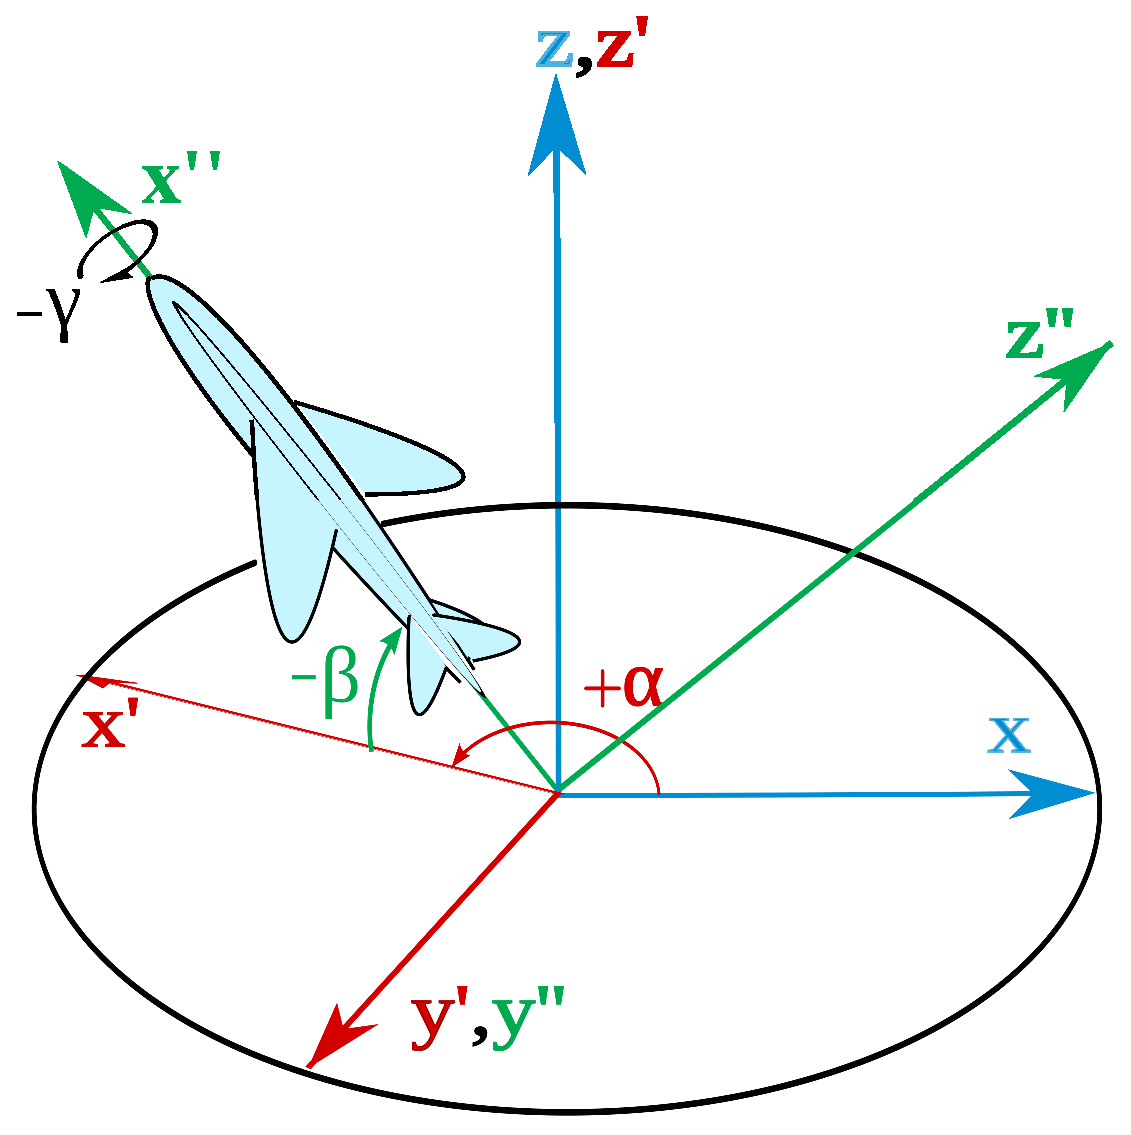
\includegraphics[width=8cm]{figures/tait_bryan.eps}
    \caption{$z-y'-x''$ rotation using Tait-Bryan angles. Figure modified from original image created by Wikipedia user Juansempere.}
    \label{fig:tait_bryan}
\end{figure}

The relationship between the unrotated Cartesian grid (machine coordinates) and the rotated and shifted Cartesian coordinates (beam grid coodinates) is given by
\begin{equation}\label{eq:xyz_to_uvw}
    \mathbf{uvw} = \mathbf{R}\cdot \mathbf{xyz} + \mathbf{origin}\,,
\end{equation}
where $\mathbf{R}$ is the rotation matrix defined by the Tait-Bryan angles, $\mathbf{uvw}$ and $\mathbf{xyz}$ are the position vectors in machine and beam grid coordinates, respectively. $\mathbf{origin}$ is the origin vector of the beam grid coordinates defined in machine coordinates.

The Tait-Bryan angles that align the beam grid with the neutral beam given two points along the beam centerline are given by
\begin{equation}
\begin{split}
    \alpha &= \arctan(v_2 - v_1,u_2 - u_1)
    \beta  &= \arcsin((w_1 - w_2)/D)
    \gamma &= 0
\end{split}
\end{equation}
with $D$ being the distance between the points.

\subsubsection{Interpolation Grid}
As mentioned, the electromagnetic fields, plasma parameters, and the fast-ion distribution function were originally mapped onto the neutral beam grid. This, however, created memory problems when the simulation domain was large or when fine spatial resolution was required. The main issue was with the mapping of the fast-ion distribution function. The mapped distribution was stored as a dense array with dimensions $(n_e,n_p,n_x,n_y,n_z)$. Increasing the number of neutral beam grid cells could very quickly outgrow the available memory. This situation was untenable as FIDASIM was starting to be used for the simulation of passive diagnostic signals from the cold edge neutrals, which fill up the entire vessel. In order to simulate the passive signals, the beam grid had to be expanded to cover a large volume. 

With the memory problems, resolution was sacrificed. To solve this problem, a 2D $R-Z$ grid was introduced. Instead of using an array look-up to determine the plasma parameters/fields within a beam grid cell, we would determine the parameters by interpolating on the 2D $R-Z$ grid. The interpolation grid solved the memory issues by exploiting the toroidal symmetry of a tokamak---more information with less space. However, with the switch to the interpolation grid we lost the ability to handle non-toroidally symmetric plasmas like stellarators. The option for 3D plasmas is currently being implemented into FIDASIM. This is being done by adding a toroidal $\phi$ variable to the interpolation grid definition. If the user does not provide $\phi$, then toroidal symmetry is assumed.

\subsection{Plasma Parameters}
In FIDASIM, the plasma parameters are mapped to the interpolation grid. This is somewhat unusual. More commonly, the plasma parameters are represented as flux functions. This is usually a good choice; however, there are a few scenarios where a flux function is not the best choice. For example, in tokamak discharges with high torque the plasma tends to move out toward the wall, a consequence of the plasma angular momentum. This can cause a mismatch in the plasma densities at the high and low field sides of a flux function. Additionally, the cold edge neutrals cannot be a flux function. There is also a matter of which flux label to support---$\psi$ or $\rho$---and how to deal with regions outside the separatrix. Mapping onto the interpolation grid was the most general choice that fixed the aforementioned issues.

FIDASIM takes in 2D profiles of the following plasma parameters: the electron density ($n_e\;\rm{cm^{-3}}$), the ion and electron temperature ($T_{i/e}\;\rm{keV}$), the plasma rotation ($\vec{v}\;\rm{cm/s}$) in cylindrical coordinates, the effective charge $Z_{eff}$, and the cold edge neutral density ($n_{cold}\;\rm{cm^{-3}}$). Within FIDASIM, the impurity and ion densities are calculated from the user supplied inputs by manipulating the quasineutrality and $Z_{eff}$ formulas:
\begin{equation}
\begin{split}
    n_{imp} &= \frac{Z_{eff} - 1}{Z\,(Z-1)} n_e, \\
    n_i &= n_e - Z\,n_{imp}\,,
\end{split}
\end{equation}
where $Z$ is the charge number of the main impurity species.
\begin{figure}[h!]
    \centering
    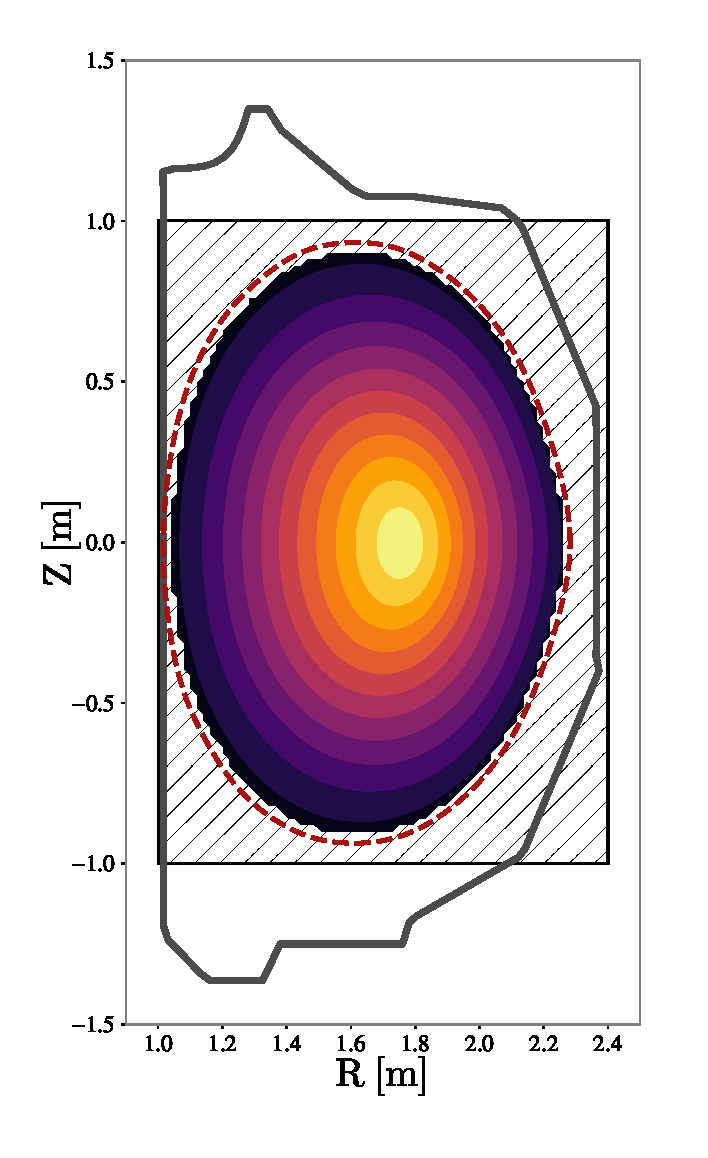
\includegraphics[width=8cm]{figures/te_cross_section.eps}
    \caption{Electron Temperature mapped onto the interpolation grid. Outside the separatrix (dashed red line) the plasma parameters are not set, i.e. the mask variable is set to 0.}
    \label{fig:te_mask}
\end{figure}
One complication that arises by not using flux functions is knowing when particles are outside the region where the plasma parameters are defined. FIDASIM uses a Boolean mask to indicate the location of the edge of the plasma. If the plasma parameters are defined at a given (R,Z), then the mask is one, otherwise, it is set to zero. Figure \ref{fig:te_mask} demonstrates the masking. For this particular time-slice the profiles were only provided up to the separatrix so the mask was set to one inside the separatrix and zero outside.

\subsection{Electromagnetic Fields}
In tokamaks, the electromagnetic fields are determined by solving the Grad-Shafranov equation
\begin{equation}\label{eq:grad_shafranov}
    \Delta^* \psi = - \mu_0 R^2 \frac{dp}{d\psi} - \frac{1}{2}\frac{dg^2}{d\psi}\,,
\end{equation}
where $\Delta^*$ is the elliptic operator, $p(\psi)$ is the pressure, $g(\psi)$ is the poloidal current, and $\psi(R,Z)$ is the poloidal flux function.
The Grad-Shafranov equation is the equilibrium equation in ideal magnetohydrodynamics (MHD) for a two dimensional plasma. While FIDASIM does not solve this equation, electing to simply map the magnetic and electric fields in cylindrical coordinates onto the interpolation grid, it is useful to know how to extract the various fields from the poloidal flux so they can be used by FIDASIM.

The magnetic field, $\vec{B}$, in cylindrical coordinates is given by
\begin{equation}\label{eq:bfield}
\begin{split}
    B_R &=  \frac{1}{R}\frac{\partial \psi}{\partial Z}, \\
    B_Z &= -\frac{1}{R}\frac{\partial \psi}{\partial R}, \\
    B_{\phi} &= \frac{g(\psi)}{R}.
\end{split}
\end{equation}
The plasma current, $\vec{J}$, in cylindrical coordinates is given by
\begin{equation}\label{eq:jfield}
\begin{split}
    J_R &= -\frac{1}{\mu_0 R}\frac{\partial g}{\partial \psi} \frac{\partial \psi}{\partial Z}, \\
    J_Z &= \frac{1}{\mu_0 R}\frac{\partial g}{\partial \psi} \frac{\partial \psi}{\partial R}, \\
    J_{\phi} &= -R \frac{\partial p}{\partial \psi} - \frac{g(\psi)}{\mu_0 R}\frac{\partial g}{\partial \psi}.
\end{split}
\end{equation}
The plasma current is not used by FIDASIM, however, it is useful to know the sign of the dot product of the magnetic field and the plasma current, $\sigma = \rm{sign}(\vec{B}\cdot\vec{J})$, known as the pitch sign convention. This will become useful when we discuss the fast-ion distribution function.

To maintain force balance, a radial electric field, $E_r$, is induced. The electric field in cylindrical coordinates is given by
\begin{equation}\label{eq:efield}
\begin{split}
    E_R &= -R \frac{B_{pol}}{|\nabla \psi|} \frac{\partial \Phi}{\partial \psi} \frac{\partial \psi}{\partial R},\\
    E_Z &= -R \frac{B_{pol}}{|\nabla \psi|} \frac{\partial \Phi}{\partial \psi} \frac{\partial \psi}{\partial Z},\\
    E_{\phi} &= 0,
\end{split}
\end{equation}
where $\Phi(\psi)$ is the electric potential, and the poloidal magnetic field is given by $B_{pol} = \sqrt{B_R^2 + B_Z^2}$.


\subsection{Fast-ion Distribution}
Simulating the signals generated by a theoretical fast-ion distribution is FIDASIM's \textit{raison d'\^etre}, its reason for being. It is, therefore, important that FIDASIM is able to support multiple types of distributions.
Internally, FIDASIM can represent fast-ions using two different 6D coordinate systems. The most commonly used is the guiding center coordinates: the kinetic energy, $E$, the pitch of the fast ion with respect to the magnetic field, $p$\footnote{There are two different definitions of pitch that are used: pitch with respect to the magnetic field, $p = \vec{v}\cdot\vec{B}/(||\vec{v}||\,||\vec{B}||)$, and pitch with respect to the plasma current, $p = \vec{v}\cdot\vec{J}/(||\vec{v}||\,||\vec{J}||)$. To convert between the two conventions one only needs to multiply the pitch with the pitch sign convention, $\sigma$, discussed previously.}, the major radius, $R$, the elevation, $Z$, and the gyro and toroidal angles $\gamma$ and $\phi$. Less frequently used is the cylindrical coordinate system: $v_r$, $v_z$, $v_\phi$, $R$, $Z$, and $\phi$.
The coordinate system that FIDASIM uses depends on the type of the distribution that was supplied by the user; of which there are two(formerly one): guiding-center distribution functions, $F(E,p,R,Z)$, and Monte Carlo particle distributions.

\subsubsection{Guiding-center Fast-ion Distribution Function}
Like the plasma parameters, the fast-ion distribution function is mapped onto the interpolation grid (Fig. \ref{fig:fast_ion_distribution}). 
\begin{figure}
    \centering
    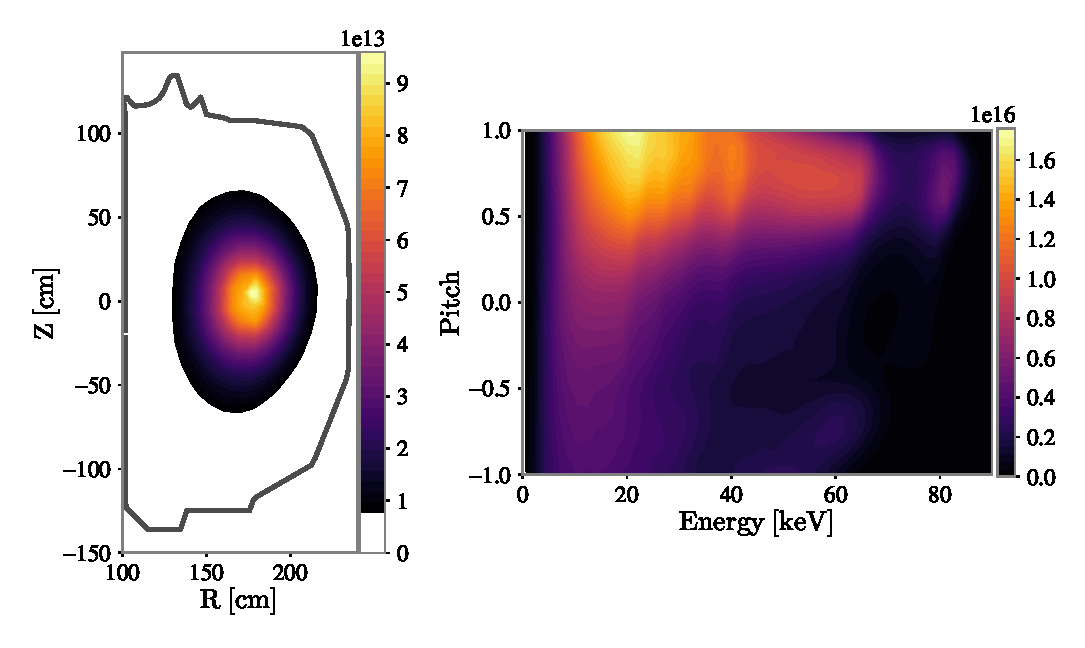
\includegraphics[width=13cm]{figures/fast_ion_distribution.eps}
    \caption{Projection of the guiding-center fast-ion distribution function for DIII-D discharge \#171469 at 1360 ms. Left: Fast-ion density: $F(R,Z)=\iint F(E,p,R,Z)\,dE\,dp$. Right: Fast-ion velocity-space distribution: $F(E,p)=\iint F(E,p,R,Z)\,R\,dR\,dZ$. Pitch is defined relative to the plasma current.}
    \label{fig:fast_ion_distribution}
\end{figure}
It is assumed that the distribution is toroidally symmetric and the gyro-angle is distributed uniformly, $\gamma \sim \mathcal{U}(0,2\pi)$.
In this form, the total number of fast-ions is given by
\begin{equation}\label{eq:f_ntot}
    N_{f} = 2\pi \iiiint F(E,p,R,Z) R\,dE\,dp\,dR\,dZ.
\end{equation}
The integration over the gyro-angle is included in the definition of $F$.

\subsubsection{Monte Carlo Distributions}
A Monte Carlo distribution is defined by a set of $N_p$ Monte Carlo (MC) particles each with a set of attributes according to the coordinate system used. Guiding-center MC particles have a kinetic energy, pitch, R, Z, and weight ($w$). The full-orbit MC particles have a velocity in cylindrical coordinates, $\vec{v} = [v_r,v_z,v_\phi]$, R, Z, and weight.
For both types of MC distributions, toroidal symmetry is assumed and for the guiding-center MC distribution it is assumed that the gyro-angle is distributed uniformly.
The weights of the particles are chosen such that the total number of fast ions is given by
\begin{equation}\label{eq:mc_ntot}
    N_{f} = \sum_i^{N_{p}} w_i \,.
\end{equation}
Since the particle weights include an implicit integration over the entire toroidal range, $[0,2\pi)$, for certain diagnostics, the weights are scaled by $\Delta \phi/2\pi$ where $\Delta \phi$ is the toroidal range of the simulation determined by the intersection of the MC particle with the neutral beam grid. This is done so $\phi$ can be efficiently sampled in a region where it is possible for signal to be produced, i.e. where there are neutrals with which to charge exchange.

\subsection{Atomic Tables}
As a neutral particle travels through a plasma, it undergoes several different types of interactions
\begin{itemize}
    \item charge exchange with Hydrogen and impurities
    \item excitation with electrons, Hydrogen, and impurities
    \item ionization with electrons, Hydrogen, and impurities
\end{itemize}
These cross sections, as well as Maxwellian averaged reaction rates, are pre-computed over a range of logarithmically spaced collision energies and target temperatures. The sources of all the cross sections are given in Appendix \ref{app:cross_sections}. 
However, some of the atomic transitions needed by FIDASIM are not available. In particular, FIDASIM needs the n/m-resolved charge exchange cross sections. While certain transitions are available through ADAS\cite{adas}, others are not, as such, certain approximations are needed to fill out the table.

For instance, we use the equivalence principle (reversibility formula) to mirror the known ADAS cross sections.
\begin{equation}\label{eq:equilvalence}
    \sigma(n_f \rightarrow n_i) = \frac{E_i}{E_f}\frac{n_i^2}{n_f^2}\sigma(n_i \rightarrow n_f)
\end{equation}
This, however, is insufficient to completely fill out the needed transitions.
Fortunately, since the \textit{total} cross sections for a transition $n \rightarrow m$ are given by Janev\cite{janev2003collision}, we can make the assumption that the probability of a transition decreases exponentially with the difference in energy between the levels. So long as we make sure the total cross section remains unchanged, we can "spread" the total cross section among the different unknown transitions.
A summary of the various approximations used in the charge exchange tables is given in Table \ref{tab:cx_sources}.
\begin{table}[ht]
\centering
\caption{Charge exchange cross section sources. Total cross sections for $n>4$ are not available so the $n=4$ total cross sections are used. The $m$ levels are normalized to the Janev\cite{janev2003collision} tables for consistency. Spreading is done over the $m$ values/rows}
\label{tab:cx_sources}
\begin{tabular}{c|c|c|c|c|c|c|c}
\textbf{n/m}        & \textbf{1}                          & \textbf{2}                          & \textbf{3}                          & \textbf{4}                    & \textbf{5}                    & \textbf{6}                    & \textbf{Total}  \\ \hline
\textbf{1} & {\color[HTML]{CB0000} ADAS}         & {\color[HTML]{CB0000} ADAS}         & {\color[HTML]{CB0000} ADAS}         & {\color[HTML]{CB0000} ADAS}   & {\color[HTML]{00009B} Spread} & {\color[HTML]{00009B} Spread} & Janev(n=1)      \\ \hline
\textbf{2} & {\color[HTML]{036400} Equivalence}  & {\color[HTML]{CB0000} ADAS}         & {\color[HTML]{CB0000} ADAS}         & {\color[HTML]{00009B} Spread} & {\color[HTML]{00009B} Spread} & {\color[HTML]{00009B} Spread} & Janev(n=2)      \\ \hline
\textbf{3} & {\color[HTML]{036400} Equivalence} & {\color[HTML]{CB0000} ADAS}         & {\color[HTML]{CB0000} ADAS}         & {\color[HTML]{CB0000} ADAS}   & {\color[HTML]{CB0000} ADAS}   & {\color[HTML]{00009B} Spread} & ADAS/Janev(n=3) \\ \hline
\textbf{4} & {\color[HTML]{036400} Equivalence} & {\color[HTML]{036400} Equivalence} & {\color[HTML]{036400} Equivalence} & {\color[HTML]{00009B} Spread} & {\color[HTML]{00009B} Spread} & {\color[HTML]{00009B} Spread} & Janev(n=4)      \\ \hline
\textbf{5} & {\color[HTML]{00009B} Spread}       & {\color[HTML]{036400} Equivalence} & {\color[HTML]{036400} Equivalence} & {\color[HTML]{00009B} Spread} & {\color[HTML]{00009B} Spread} & {\color[HTML]{00009B} Spread} & Janev(n=4)      \\ \hline
\textbf{6} & {\color[HTML]{00009B} Spread}       & {\color[HTML]{036400} Equivalence} & {\color[HTML]{036400} Equivalence} & {\color[HTML]{00009B} Spread} & {\color[HTML]{00009B} Spread} & {\color[HTML]{00009B} Spread} & Janev(n=4)     
\end{tabular}
\end{table}

In addition to the cross sections, we also need the beam-plasma reaction rates, which we can readily calculate from the cross sections. With the assumption that the fast-ion density is small compared to the thermal density (below \%20), the beam-plasma reaction rate is given by an average over a Maxwellian,
\begin{equation}\label{eq:full_reaction_rate}
    \langle \sigma v \rangle = \iint \sigma(E_{rel}) ||\mathbf{v} - \mathbf{v'}|| \delta(\mathbf{v'}-\mathbf{v}_B) \left [ \frac{m_T}{2\pi kT} \right ]^{\frac{3}{2}} e^{-\frac{m_T}{2kT}(\mathbf{v}\cdot\mathbf{v})} d\mathbf{v}'\,d\mathbf{v} ,
\end{equation}
where $\mathbf{v}_B$ is the beam velocity, $m_T$ is the mass of the plasma/target species, and $T$ is the plasma temperature. Finding the reaction rate requires integrating over a range of velocities. This creates a slight inconvenience when tabulating the rates since the velocities would change depending on the temperature. To ameliorate this, a simplified form of Equation \ref{eq:full_reaction_rate} that uses normalized velocities, $u_{r/z}$, is used to calculate the reaction rates. The simplified reaction rate equation takes the form
\begin{equation}\label{eq:reaction_rate}
\langle \sigma v \rangle = \frac{2}{\sqrt{\pi}}\sqrt{\frac{2kT}{m_T}} \iint \sigma(E_{rel}) \sqrt{u_r^2 + \left (u_z - \sqrt{\frac{E_B m_T}{m_B kT}}\right)^2}  e^{-(u_r^2 + u_z^2)}u_r \,du_r\,du_z\,,
\end{equation}
where $m_B$ and $E_B$ is the mass and energy of the beam species respectively. In terms of the normalized velocities, the relative energy of collision, $E_{rel}$ is given by
\begin{equation}\label{eq:e_rel}
E_{rel} = \mu \frac{kT}{m_T} \left ( u_r^2 + \left(u_z - \sqrt{\frac{E_B m_T}{m_B kT}}\right)^2 \right )\,,
\end{equation}
where $\mu$ is the reduced mass of the species.
To find the reaction rate, Equation \ref{eq:reaction_rate} is integrated from a normalized velocity of $-4$ to $4$ in both the $r$ and $z$ directions.
The full derivation of the reaction rate equation is given in Appendix \ref{app:reaction_rate}. 

%===============================================================================
%===============================================================================
%===============================================================================
\section{Simulation of Neutral Populations}
The neutral densities are an important part of the fast-ion diagnostics forward models and require careful modeling.
There are four neutral populations that FIDASIM simulates: the neutral beam which consists of full, half, and third energy components, the thermal halo, fast neutrals, and the cold edge neutrals.
With the exception of the cold edge neutrals, the algorithm for simulating the different neutral populations are remarkably similar, differing only in their initial conditions and possible trajectories through the plasma.

\subsection{Neutral Particle Trajectories}
The amount of neutrals produced by a source is distributed among the particle trajectories produced by the source. The trajectories the neutral particles take is determined by the local neutral velocity distribution, which is taken to be the ion distribution for neutrals born of charge exchange. The number of trajectories used in the calculations, $N_t$, is a user input and is typically set to be very large ($\sim10^6$) to best represent the true distribution. The more trajectories used, the more accurate the result.

The neutral particles trajectory through the neutral beam grid is used prolifically within FIDASIM as the time spent in each cell is needed to solve the collisional radiative model (COLRAD)(Eq. \ref{eq:colrad}, \ref{eq:neutral_population}), which determines how the neutrals are distributed along the cells in the track. Summing the contributions of each trajectory determines the total spatial profile of the neutrals. The tracking through the beam grid could be done at the same time as COLRAD, but pre-computing the track allows us to be able to short-circuit certain calculations; avoiding the computationally expensive COLRAD calculation. For instance, in the FIDA calculation, if a fast neutral doesn't cross a line of sight, it can't contribute signal; therefore, there is no need for the full calculation.

The particle tracking algorithm is as follows.
Each 3D cell in a grid is defined by 6 surfaces. In the case of a Cartesian grid, the cell is defined by the intersection of 6 planes, for a cylindrical grid it is defined by 4 planes and 2 cylinders. Given an initial starting point and velocity, the time it takes to intersect each surface is calculated. The smallest non-negative time, $t_{min>0}$, is the time spent in the cell. Information about the cell is collected and the neutral particle is advanced by $t_{min>0}$. This process repeats until the neutral particle exits the grid.

\subsection{Beam Neutrals}
The geometry of a neutral beam is defined by a source position and an axis such that a point along the beam centerline is defined as
\begin{equation}\label{eq:nbi_geom}
    \vec{C}(t) = \vec{s} + \vec{a} \cdot t\,,
\end{equation}
where $\vec{C}(t)$ is the position along the centerline parameterized by $t$, $\vec{s}$ is the source position, and $\vec{a}$ is the axis. The ion source is defined by its shape (circular or rectangular), size (half width and half height), vertical and horizontal focal lengths, and an energy dependent divergence. 

The trajectory of a beam neutral is determined by the following equations:
\begin{equation}\label{eq:beam_trajectory}
    \begin{split}
        v_x &= 1  \\
        v_y &= v_x\left(-\frac{y_s}{f_y} + \tan(\theta_y)\right),\quad \theta_y \sim \mathcal{N}(0,\beta_y^2) \,,\\
        y_z &= v_x\left(-\frac{z_s}{f_z} + \tan(\theta_z)\right),\quad \theta_z \sim \mathcal{N}(0,\beta_z^2)\,,
    \end{split}
\end{equation}
where $v_x$ points towards the plasma, $y_s$ and $z_s$ are random positions on the source plate in the horizontal and vertical directions respectively, $f_{y/z}$ are the focal lengths, and $\beta_{y/z}$ are the divergences. Examples of the different trajectories generated by the above equations are shown in Figure \ref{fig:beam_divergence}.
\begin{figure}[ht]
    \centering
    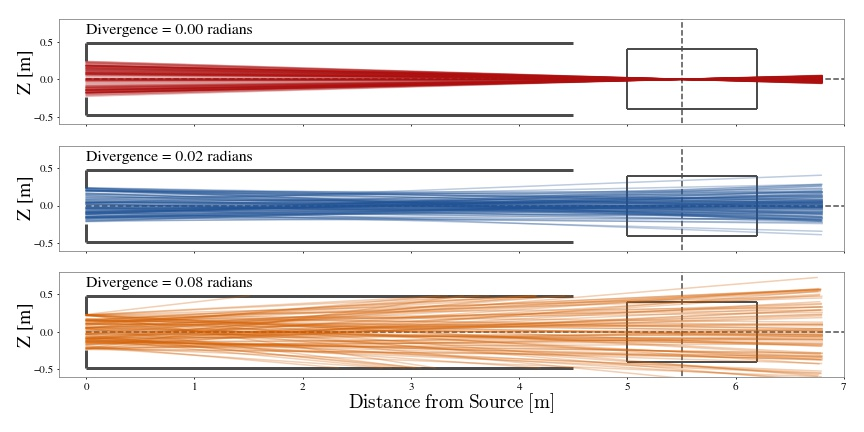
\includegraphics[width=15cm]{figures/beam_divergence.jpg}
    \caption{The effects of different beam divergences on beam particle trajectories. Focal length (dashed vertical line) is fixed at 5.5 m.}
    \label{fig:beam_divergence}
\end{figure}
Not shown in the above figure are the beam aperture(s), which collimate the neutral beam. Apertures are represented in FIDASIM by their shape (circular or rectangular), size (half width and half height), offsets relative to the +x aligned beam centerline, and their distance from the source grid. It is assumed that the plane of the aperture(s) is parallel to the plane of the source grid.

With the neutral beam geometry, we are able to approximate the beam neutral velocity distribution at a given point. The beam neutral velocity distribution, $f_b$, in beam grid coordinates is proportional to
\begin{equation}\label{eq:beam_distribution}
    f_b(\vec{v}) \propto \frac{\cos^2(\theta_y)\cos^2(\theta_z)}{2\beta_y\beta_z}\exp\left(-\left(\frac{\theta_y^2}{2\beta_y^2} + \frac{\theta_z^2}{2\beta_z^2}\right)\right)I(\vec{v},y_s,z_s)\,,
\end{equation}
where $I(\vec{v},y_s,z_s)$ is a function that indicates that the trajectory is possible and the angles $\theta_{y/z}$ are found via Equation \ref{eq:beam_trajectory}. Normalization aside, in vacuum, the above equation is exact; however, attenuation within the plasma weights each possible trajectory differently, incurring a slight error. Although not done in FIDASIM, appending a trajectory dependent attenuation factor to Equation \ref{eq:beam_distribution} would correct for it.

During the acceleration phase of neutral beam injection, multiple atomic and molecular species are accelerated to the same kinetic energy,$E_{inj}$. During the neutralization phase, the molecular species are split apart, creating neutral populations with different energies: $E_{inj}$, $E_{inj}/2$, and $E_{inj}/3$. These different beam populations are called the Full, Half, and Third energy components respectively.
Each beam component attenuates differently in the plasma and needs to be treated separately.
\begin{figure}[h!]
    \centering
    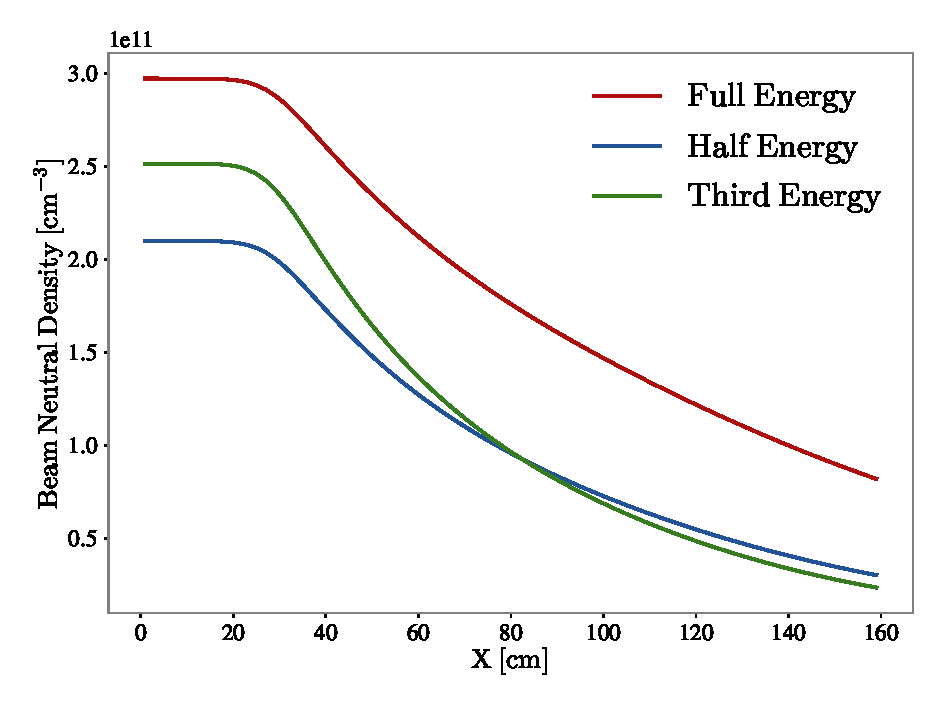
\includegraphics[width=10cm]{figures/beam_attenuation.eps}
    \caption{Attenuation of the different beam species for a DIII-D discharge. Density is summed over the y and z directions.}
    \label{fig:beam_attenuation}
\end{figure}
For a single beam trajectory, it is assumed that the beam neutral for the i$_{th}$ energy component is in the ground ($n=1$) state with initial population flux given by
\begin{equation}\label{eq:nb_flux}
    f_1(t=0)|_i = \left. \frac{d n_1}{dt}\right\rvert_i = \frac{C_i}{N_t} \cdot \frac{d n_{tot}}{dt}\,,
\end{equation}
where $C_i$ is the components current fraction, $N_t$ is the number of beam trajectories, and $dn_{tot}/dt$ is the total population flux of neutrals given by
\begin{equation}\label{eq:tot_flux}
    \frac{d n_{tot}}{dt} = \frac{P_{inj}}{\sum_i^3 C_i E_{inj}/i}\,,
\end{equation}
where the numerator, $P_{inj}$, is the total beam power and the denominator is the average beam energy.
The current fractions are a measured quantity that are specific to a neutral beam. For DIII-D's neutral beams, the current fractions are a function of the injection energy and are given by
\begin{equation}\label{eq:d3d_cfracs}
\begin{split}
    C_{1}(E_{inj}) &= -0.109171 + 0.0144685\, E_{inj} - 7.83224\times10^{-5}\, E_{inj}^2 \\
    C_{2}(E_{inj}) &= 0.0841037 + 0.0025516\, E_{inj} - 7.42683\times10^{-8}\, E_{inj}^2 \\
    C_{3}(E_{inj}) &= 1 - C_{1} - C_{2}
\end{split}
\end{equation}

As the neutral travels through the grid, it will be attenuated by the plasma and neutrals will be deposited in each cell it crosses. Figure \ref{fig:beam_attenuation} shows the attenuation of the different beam species as they travel through the plasma. To get the total beam density, the above process is repeated for the $N_t$ beam trajectories and the results summed. Figure \ref{fig:beam_density}a shows the neutral beam profile.
\begin{figure}[h!]
    \centering
    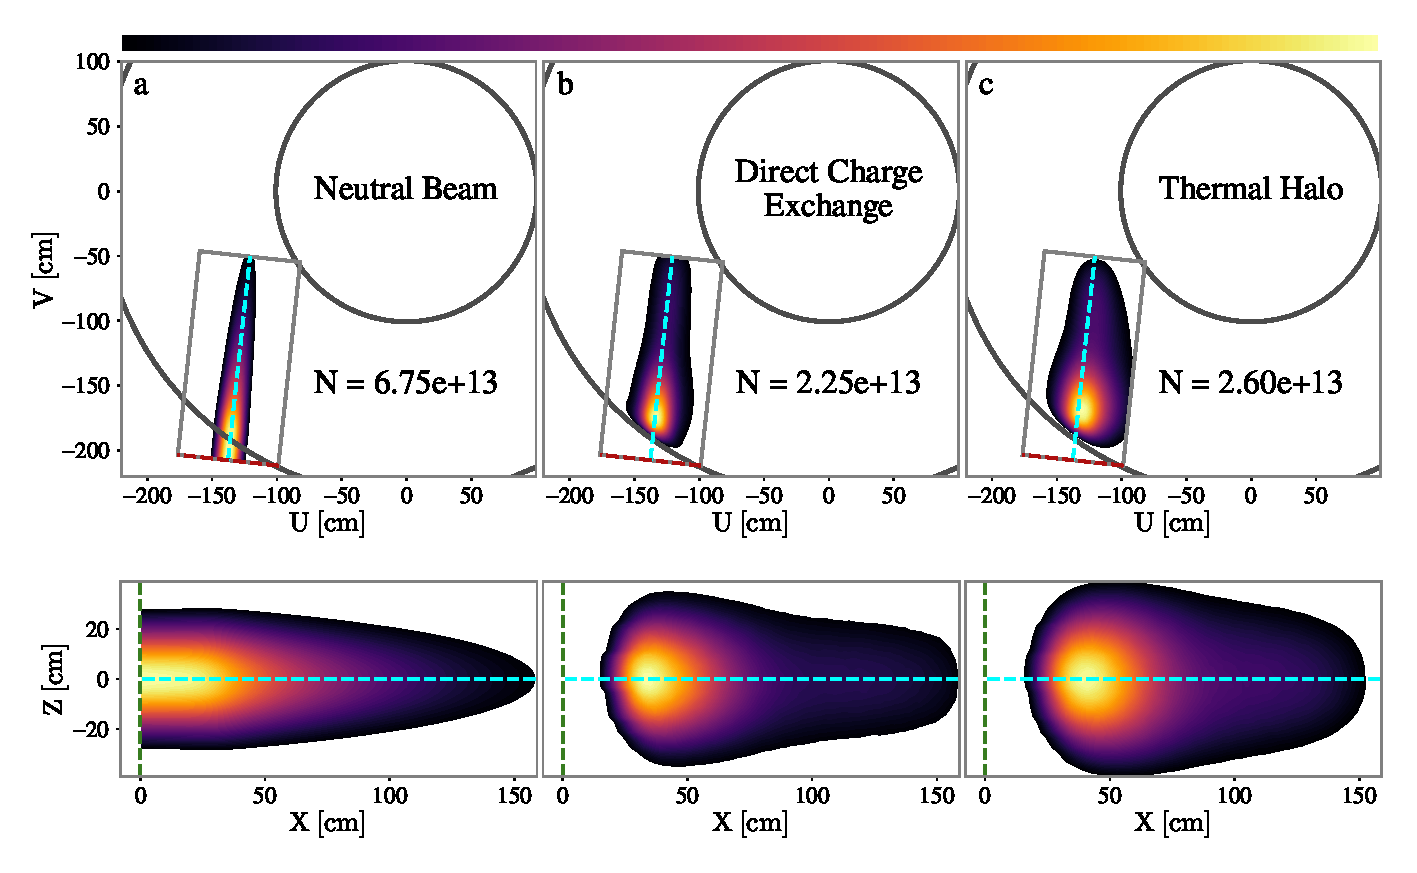
\includegraphics[width=16cm]{figures/beam_density.eps}
    \caption{Neutral profiles for the neutral beam (Column a), direct charge exchange (DCX) (Column b), and thermal halo (Column c). Top row: 2D profiles in machine coordinates, integrated over $W$. Bottom row: 2D profiles in beam grid coordinates, integrated over $Y$. The beam grid axes are color coded: $X$ axis (dashed cyan), $Y$ axis (dashed red), and $Z$ axis (dashed green) The number of neutrals in each population is listed. The colormap on top increases from left to right. The beam geometry is the 210RT neutral beam on DIII-D.}
    \label{fig:beam_density}
\end{figure}

\subsection{Direct Charge Exchange and Halo Neutrals}
Beam neutrals, $H_b$, can undergo charge exchange with thermal ions, $H_{th}^+$, creating a new neutral population. This population is called the direct charge exchange (DCX) neutrals. The initial population flux for a DCX neutral born in a cell with beam density, $\mathbf{d}_i$, is given by
\begin{equation} \label{eq:dcx_rates}
    \mathbf{f}(t=0) = \frac{N_{th}}{N_{t}}\sum_{i=1}^3 \left [ \int \mathbf{X}(\mathbf{v}_{DCX} - \mathbf{v}) \cdot \mathbf{d}_i\, ||\mathbf{v}_{DCX} - \mathbf{v}||\, f_i(\mathbf{v})\, d\mathbf{v} \right ]\,,
\end{equation}
where $\mathbf{X}$ $[cm^2]$ is a matrix of the charge exchange cross sections, $f_i$ is the velocity distribution of the $i^{th}$ beam energy component, $\mathbf{v}_{DCX}$ is the DCX neutral velocity, $N_{th}$ is the number of thermal ions in the cell, and $N_{t}$ is the number of trajectories the DCX neutral could take. The trajectories are determined from the local thermal ion velocity distribution that takes the form of a shifted Maxwellian.

After the initial population flux is determined, the DCX neutral travels ballistically and deposits neutrals along its trajectory in accordance with the collisional radiative model. The DCX density produced by a cell is determined by summing the contributions from each DCX trajectory. The total DCX density is calculated by repeating the above process for every cell that contains a beam neutral.

Likewise, the DCX neutrals can also undergo charge exchange with the thermal ions, creating a new neutral population that will then also undergo charge exchange with the thermal ions. The process of a neutral population charge-exchanging with the thermal ions can repeat ad infinitum; each new generation producing fewer neutrals than the generation before it. The overall effect is a thermal Halo of neutrals surrounding the neutral beam. The iterative process is demonstrated in Equation \ref{eq:dcx_halo_iteration}.
\begin{equation}\label{eq:dcx_halo_iteration}
\begin{split}
\rm{DCX\,\,:} \quad &H_{th_0}^+ + H_b \rightarrow H_{th_0} + H_b^+\\
\rm{Halo\,:} \quad &H_{th_1}^+ + H_{th_0} \rightarrow H_{th_1} + H_{th_0}^+\\
\rm{Halo\,:} \quad &H_{th_2}^+ + H_{th_1} \rightarrow H_{th_2} + H_{th_1}^+ \\
\vdots \\
\rm{Halo\,:} \quad &H_{th_k}^+ + H_{th_{(k-1)}} \rightarrow H_{th_k} + H_{th_{(k-1)}}^+
\end{split}
\end{equation}
The process for calculating the Halo neutrals is similar to the DCX calculation, just repeated until the amount of halo neutrals produced in a generation is 1\% of the initial seed population, which is the DCX neutrals. The other difference between the Halo and the DCX calculation is how the initial population flux is set.
The initial population flux for a k$^{th}$ generation Halo neutral born in a cell with neutral density, $\mathbf{d}_{k-1}$, is given by
\begin{equation} \label{eq:dcx_rates}
    \mathbf{f}(t=0)|_k = \frac{N_{th}}{N_{t}} \left [ \int \mathbf{X}(\mathbf{v}_{Halo} - \mathbf{v}) \cdot \mathbf{d}_{k-1}\, ||\mathbf{v}_{Halo} - \mathbf{v}||\, f_{k-1}(\mathbf{v})\, d\mathbf{v} \right ]\,,
\end{equation}
where $N_{t}$ is the number of neutral trajectories, $\mathbf{v}_{Halo}$ is the Halo neutral velocity which is drawn from a shifted Maxwellian, and $f_{k-1}$ is the the neutral velocity distribution of the $(k-1)$ Halo generation, which is also a shifted Maxwellian. In both cases, the Maxwellians are parameterized by the local ion temperature and rotation.
The DCX and Halo neutral density profiles are shown in Figures \ref{fig:beam_density}b-c.

\subsection{Fast Neutrals}
Fast neutral are born of charge exchange reactions between the previously discussed neutral populations and the fast ions. 
The initial population flux for a fast neutral is given by
\begin{equation}\label{eq:fast_rates}
    \mathbf{f}(t=0) = \frac{N_f}{N_{t}}\sum_k \left [ \int \mathbf{X}(\mathbf{v}_f - \mathbf{v}) \cdot \mathbf{d}_k\, ||\mathbf{v}_f - \mathbf{v}||\, f_k(\mathbf{v})\, d\mathbf{v} \right ]\,,
\end{equation}
where $\mathbf{X}$ $[cm^2]$ is a matrix of the charge exchange cross sections, $\mathbf{d}_k$ $[cm^{-3}]$ is the densities vector of the $m$ energy levels of the donor neutral, $f_k$ is the velocity distribution of the $k^{th}$ neutral population, and lastly $N_f$ and $N_t$ are the number of fast ions in the cell and the number of possible trajectories the fast ion can take, respectively. The trajectories a fast ion can take are determined by the fast-ion distribution function. Combining the contributions for each trajectory gives the local fast neutral profile. Summing over cells gives the total fast neutral density profile.

In order to use a Monte Carlo distribution, the $N_f/N_t$ factor in Equation \ref{eq:fast_rates} is replaced with the fast ions weight, $w$. This can be justified by comparing Equation \ref{eq:fast_rates} to Equation \ref{eq:cx_rates} which is the initial population flux for a single fast ion. Upon inspection, it becomes apparent that the factor $N_f/N_t$ is the number of fast-ions on a specific trajectory which is equivalent to the Monte Carlo particle weight.

In contrast with the other neutral populations, the fast neutral population is only used in the calculation of the FIDA and NPA signals. Therefore, only the fast neutral trajectories that contribute signal are calculated. This significantly reduces the computational cost.

\subsection{Cold Edge Neutrals}
As mentioned in the previous section, the cold edge neutrals is a user input. However, only the $n$ integrated density is supplied; $n$-resolved densities are required for the calculation of passive signals. To determine the population of each energy level, it is initially assumed that the cold edge neutral is entirely in the ground state. Using the local plasma parameters the cold edge neutrals are then time evolved by the collisional radiative model until it reaches equilibrium. The cold edge neutrals are then distributed relative to the equilibrium population levels.

\section{Simulation of Spectra}
\begin{figure}[h!]
    \centering
    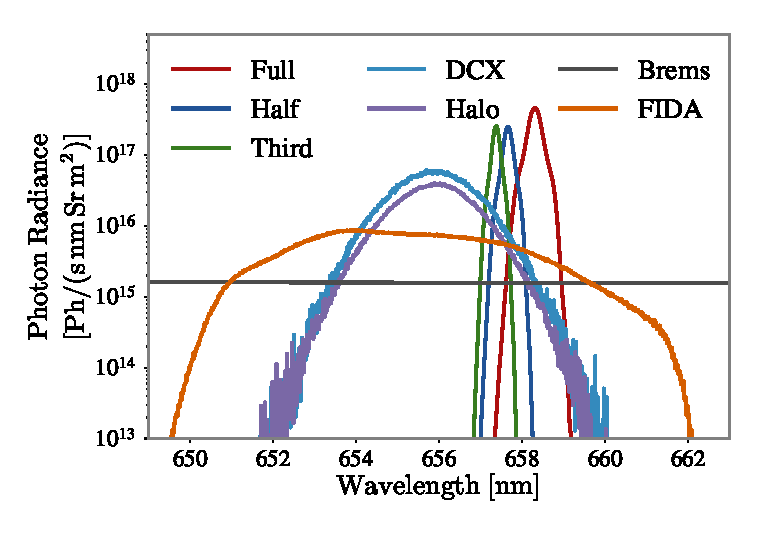
\includegraphics[width=10cm]{figures/spectra.eps}
    \caption{Spectra calculated by FIDASIM. Line of sight is viewing DIII-D 210RT neutral beam at an oblique angle in the core of the plasma.}
    \label{fig:spectra}
\end{figure}
\subsection{Spectroscopic Geometry}
Similar to the neutral beam geometry, each spectroscopic line of sight (LOS) is defined by a lens source location, an optical axis, and an optional spot size. The intersection of the LOS with the neutral beam cell is calculated using the neutral particle tracking algorithm described previously. In the original version of FIDASIM, the LOS intersections were stored in a $n_x \times n_y \times n_z \times n_{chan}$ sized grid. This caused memory issues when a large number of LOS were simulated, e.g. in a camera setup. This issue was resolved by using a sparse representation of the LOS intersections.

\subsection{Bremsstrahlung}
The largest source of background emission is visible bremsstrahlung. The local bremsstrahlung per unit wavelength is given by
\begin{equation}\label{eq:brems}
    \frac{dN_B}{d\lambda} = 7.57\times10^{-9} g\frac{n_e^2 Z_{eff}}{\lambda T_e^{1/2}}e^{-hc/\lambda T_e}\,,
\end{equation}
where $\lambda$ is the wavelength in angstroms, $n_e$ and $T_e$ is the electron density in $cm^{-3}$ and temperature in eV respectively. The gaunt factor, $g$, depends on $T_e$ and $Z_{eff}$. It can be approximated by
\begin{equation}\label{eq:gaunt}
    g = 5.542 - (3.108 - \ln(T_e/1000))(0.6905 - 0.1323/Z_{eff})\,.
\end{equation}
To calculate the total emission, the local emissivity is integrated over the line of sight.\cite{van2010imaging}

\subsection{Emission From Neutrals}
The emissions from neutrals are collected during the neutral density calculations. The photon radiance produced by a cell can be derived from Equation \ref{eq:photon_radiance} and is given by
\begin{equation}\label{eq:cell_photon_radiance}
    L_\gamma = \frac{1}{4\pi V_{cell}} L_{cell} \Phi_\gamma\,,
\end{equation}
where $V_{cell}$ and $L_{cell}$ is the volume and LOS intersection of the cell respectively, and $\Phi_\gamma$ is the photon flux given by Equation \ref{eq:photon_flux}.
The photon radiance is then distributed among the stark components in accordance with Equations \ref{eq:wavelengths} and \ref{eq:stark_intens}. Summing the spectra over the LOS cells gives the total spectra.

Calculating the neutral beam spectra during the neutral density calculation is the preferred method as it correctly models the neutral particle velocity distribution. However, in addition to the cold edge neutrals, FIDASIM offers the ability to preload the beam, DCX and halo neutral densities. In these cases, only the total photon radiance produced by a cell is known. In order to calculate the spectrum, it is assumed that the photon radiance is equally split between the neutral particles within the cell. A distribution of the neutral particle velocities within the cell is also assumed. In the case of the beam neutrals, Equation \ref{eq:beam_distribution} is used, otherwise the local ion velocity distribution is used. The spectrum is then calculated by drawing samples from the velocity distribution and averaging the resultant spectrum. The total spectra is found by summing the spectra produced over the LOS. The quality of the approximate spectrum depends on the accuracy of the underlying assumptions. Figure \ref{fig:approx_spectra} compares the approximate spectra with the full simulation.
\begin{figure}[h!]
    \centering
    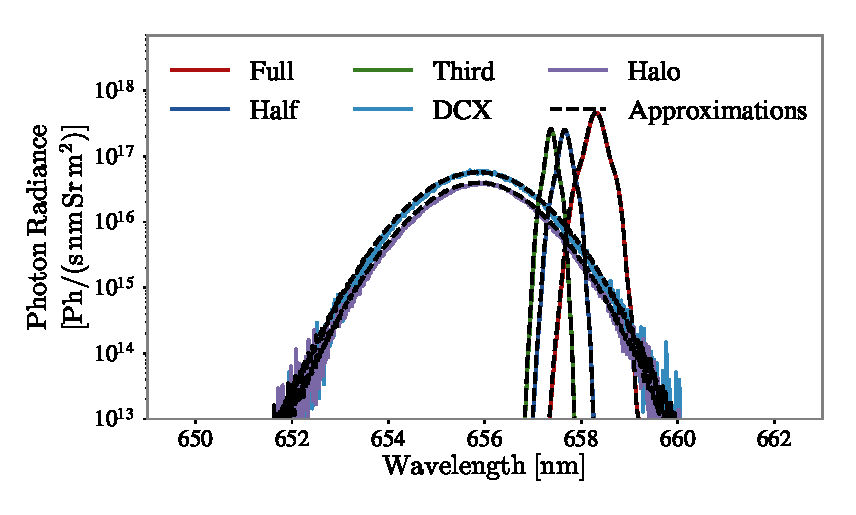
\includegraphics[width=12cm]{figures/approx_spectra.eps}
    \caption{Comparisons of full neutral beam spectra calculation (colored lines) and approximate method (black dashed overlay). The line of sight views the core region at an oblique angle.}
    \label{fig:approx_spectra}
\end{figure}

\section{Simulation of Neutral Particle Analyzers}
Neutral particle analyzers collect fast neutrals that escape the plasma. However, since most fast-neutral trajectories miss, simulating the detectors require a ridiculous number of trajectories to even have a chance of hitting the detector. Originally, FIDASIM could only use this approach, which was practically useless because of the computational cost---a single NPA simulation with good statistics could take more than a week. In the latest versions of FIDASIM, this issue has been rectified for guiding center distributions by \textit{a priori} calculating the range of trajectories that would hit the detector. This required improvements to the NPA geometry.

\subsection{NPA Geometry}
\begin{figure}[h!]
    \centering
    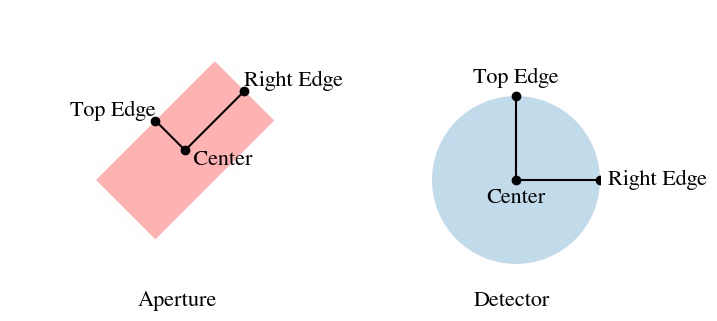
\includegraphics[width=15cm]{figures/npa_geom.jpg}
    \caption{NPA geometry definition. An aperture/detector is defined by three points, (u,v,w), which define a plane. As viewed from inside the vessel the three points are: the center, the top edge, and the right edge. The shape of the aperture/detector can either be rectangular or circular/ellipsoidal.}
    \label{fig:npa_geom}
\end{figure}
The NPA geometry in the original FIDASIM was only defined by a location, axis, and opening angle. If the entire neutral trajectory was within the cone defined by the opening angle, the neutral particle was accepted. This original definition didn't take into account the finite detector/aperture shapes and assumed rotational symmetry around the detector axis.
In newer versions of FIDASIM, the NPA geometry was changed. In the new version, the NPA detector is assumed to have an aperture and detector. Both the aperture and the detector are defined by three points which define a bounded plane: the center of the aperture/detector, the center of the top edge, and the center of the right edge. These points, along with a shape indicator, define the size of the aperture/detector as well as define a coordinate system with the +z axis normal to the plane. The apertures and detectors can be arbitrarily oriented. Figure \ref{fig:npa_geom} summarizes the NPA geometry definition.

\begin{figure}[h!]
    \centering
    \includegraphics[width=10cm]{figures/inpa.eps}
    \caption{DIII-D's imaging NPA. FIDASIM models the pinhole aperture and the stripping foil as the detector. Curved trajectories to the phosphor plate are calculated in post-processing. Image complement of Xiaodi Du.}
    \label{fig:inpa}
\end{figure}
The new NPA geometry is very flexible and can be used to describe novel NPA configurations. For instance, DIII-D's new imaging NPA (INPA)\cite{du2018inpa}, shown in Figure \ref{fig:inpa}, has a small circular pinhole aperture and a long skinny rectangular stripping foil, which is modeled as the detector.\cite{du2018inpa}

\subsection{NPA Calculation via Solid Angles}
Instead of relying on Monte Carlo trajectories to determine which fast neutrals contribute to the NPA signal, the geometric effects can be explicitly calculated\cite{stagner2014geometric}.
The geometric factor, $f_g$, of a detector is proportional to its solid angle. The geometric factor is given by
\begin{equation}
\label{eq:solid_angle}
f_g = \frac{1}{4\pi} \iint_S \frac{\mathbf{r}\cdot\hat{\mathbf{n}}\,\,dS}{r^3}\,,
\end{equation} 
where $S$ is the viewable detector area. For most cases, this equation cannot be solved analytically hence the need for Monte Carlo methods.

NPA detectors with an aligned circular aperture and detector can be described by three parameters: the aperture radius ($R_a$), the detector radius ($R_d$), and the separation between the aperture and the detector ($H$). At some positions, the aperture cuts off portions of the detector, reducing the detecting surface $S$ and complicating the solid angle calculation. Thomas \emph{et. al.} \cite{thomas1972analytical} calculated the detecting surface $S$ by projecting the ``shadow'' created by the aperture onto the detector. This ``aperture shadow'' is parametrized by the angle of incident flux $\theta$. For an isotropic distribution of incident particles, the total geometric factor of the detector is given by
\begin{equation}
\label{eq:tot_gf}
f_g= 2\pi\int_0^{\theta_{m}}S(\theta)\sin(\theta)\cos(\theta)\,d\theta\,,
\end{equation}
where $\theta_{m}$ is the maximum angle of incidence. This expression---and others like it---have been used in analyzing NPA detectors for decades. 

When simulating NPA detectors, Equation \ref{eq:tot_gf} is of limited use since it does not parametrize the aperture shadow $S$ by position. We can do this by circumscribing the aperture onto the detector plane. Defining the detector to be on the $z=0$ plane with the normal vector co-linear with the z-axis, a source at point $(x_p,y_p,z_p)$ projects a circle onto the detecting plane with radius and center given by
\begin{equation}
\label{eq:shadow_radius}
R_s = \frac{R_a z_p}{z_p - H}
\end{equation}
and
\begin{equation}
\label{eq:shadow_center}
\vec{r}_{center} = \left(\frac{H x_p}{H-z_p} , \frac{H y_p}{H-z_p} ,0\right)\,,
\end{equation} 
where $z_p > H$. Integrating over the intersection of this circle and the detector circle gives an analytic expression for the aperture shadow $S(x_p,y_p,z_p)$.

\begin{figure}[h!]
    \centering
    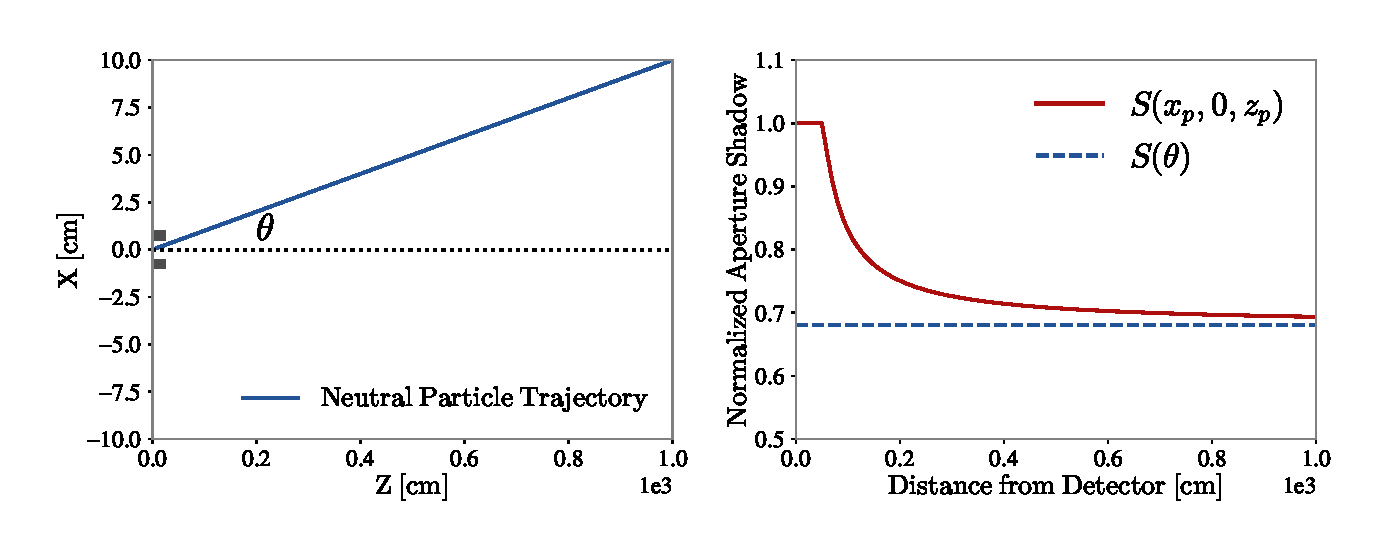
\includegraphics[width=15cm]{figures/aperture_shadow.eps}
    \caption{Left: Trajectory of a neutral particle hitting a circular NPA detector with $R_a=R_d = 0.5$ cm, and $H= 25.4$ cm. Right: Normalized aperture shadow along the particle trajectory.}
    \label{fig:shadow_compare}
\end{figure}
The two expressions for the aperture shadow ($S(\theta)$ and $S(x_p,y_p,z_p)$) should be equivalent. However, comparing the two expressions reveals a discrepancy. 
Figure \ref{fig:shadow_compare} shows that at a constant angle of incidence, the shadow area, $S(x_p,y_p,z_p)$ asymptotically approaches $S(\theta)$ as the distance from the detector increases. The discrepancy arises because the expression $S(\theta)$ implicitly assumes that the particle source is far away from the detector (far-field assumption) and can be parameterized by a single angle of incidence. 

To understand this, consider an isotropically emitting source. Far away from the detector the choice of angle of incidence $\theta$ is trivial since they are approximately the same for every trajectory that strikes the detector. When the source is near the detector, the choice of angle of incidence is not as clear since there are many possible particle trajectories each with a significantly different angle of incidence. As the particle source moves away from the detector, the possible angles of incidence approach a single value. 
However, for NPA detectors the particle source is relatively close to the detector aperture (~0.5 m); violating the requirements needed to use the $\theta$ parametrized geometric factor. Instead, a brute force application of Equation \ref{eq:solid_angle} over the aperture shadow should be used.

As mentioned, the calculation of the solid angle can be challenging; however, there is an alternative.
The geometric factor can be thought of as the probability of a particle hitting the detector from a point $\vec{p}$ above the detector. The problem of calculating the geometric factor of the detector becomes the exercise of mapping the probability density function at the source onto the detector plane $z=0$. In general, the mapping from $\mathbf{Y}$ to $\mathbf{X}$ space is done through the change in variable equation 
\begin{equation}
\label{eq:change_of_variables}
prob(\mathbf{X}) = prob(\mathbf{Y}) \times \left | \frac{\partial \mathbf{Y}}{\partial \mathbf{X}} \right|\,,
\end{equation}
where the term on the far right is the Jacobian of the transformation.\footnote{The transformation $X = H(Y)$ is subject to the constraint that $H$ is bijective and differentiable. If $H$ is not bijective Eq. \ref {eq:change_of_variables} can be extended to a summation over all the $Y$ values that correspond to a given $X$.}

In the case of NPA detectors, the transformation is from $\{\phi,\theta\}$-space, where $\phi$ and $\theta$ are the azimuthal and polar angle respectively, to $\{x,y\}$-space. For linear trajectories, the transformation is given by
\begin{equation}
\label{eq:matrix_transform}
\begin{bmatrix}
	x \\
	y \\
	0 \\
\end{bmatrix}
=
\begin{bmatrix}
	1 & 0 & \tan{\theta}\cos(\phi)\\
	0 & 1 & \tan{\theta}\sin(\phi)\\
	0 & 0 & 0\\
\end{bmatrix}
\begin{bmatrix}
	x_p \\
	y_p \\
	z_p \\
\end{bmatrix}\,,
\end{equation}
where $(x_p,y_p,z_p)$ is the position of the particle source. The Jacobian for this transformation is given by
\begin{equation}
\label{eq:jacobian}
\left | \frac{\partial(\phi,\theta)}{\partial(x,y)} \right| = \frac{z_p ((x-x_p)^2 + (y-y_p)^2)^{-1/2}}{(x-x_p)^2 + (y-y_p)^2 + z_p^2}\,.
\end{equation}
For an isotropic source, the probability density function in $\{\phi,\theta\}$-space is given by 
\begin{equation}
\label{eq:source_pdf}
prob(\phi,\theta) = \frac{1}{4\pi} \sin(\theta)\,.
\end{equation}
Plugging equation \ref{eq:source_pdf} and \ref{eq:jacobian} into the change of variable equation and integrating over the aperture shadow $S(x_p,y_p,z_p)$ yields the geometric factor,
\begin{equation}
\label{eq:prob_geo}
f_g = \frac{1}{4\pi}\iint_S\frac{z_p\,\, dS}{((x-x_p)^2 + (y-y_p)^2 + z_p^2)^{3/2}}\,.
\end{equation}
\begin{figure}[h!]
    \centering
    \includegraphics[width=15cm]{figures/npa_prob.eps}
    \caption{Geometric Factor/Probability of hitting DIII-D's solid state NPA detector. Probability evaluated on the $y=0$ plane. Dashed lines are detecting limits.}
    \label{fig:npa_prob}
\end{figure}

For circular detectors, the detecting region can be found by using Equations \ref{eq:shadow_radius}-\ref{eq:shadow_center}; however, for arbitrarily oriented and shaped apertures/detectors the detecting region is determined by checking whether the trajectories from the source to a point on the detector passes through the aperture.
Figure \ref{fig:npa_prob} shows the geometric factors/probabilities of hitting one of DIII-D's solid state NPA detector. As can be seen, the probability is extremely small and demonstrates why the traditional method of calculating NPA signal is inefficient. 

With the probabilistic formulation, we are also able to find the average strike point on the detector. Combined with the fast-neutral starting point, we are then able to calculate the pitch, $p_t$, of the fast neutral as well as a representative trajectory from the source to the detector. With this information, we can establish the initial population flux of the fast-neutral with energy, $E$, which is the same as Equation \ref{eq:fast_rates} with the $N_f/N_t$ term replaced with $2*F(E,p_t,R_s,Z_s)*f_g*V_{cell}*dE$; the factor of two is needed to convert the fast-ion distribution units from $N_f/(dE\,dp\,dR\,dZ)$ to $N_f/(dE\,dR\,dZ\,d\Omega/4\pi)$, i.e. to use the same units as the geometric factor. The collisional radiative model is then solved along the track and total population flux is then stored. Figure \ref{fig:npa_flux} shows the fast-neutral energy flux incident on the stripping foil for the DIII-D's INPA diagnostic. Using this approach, the computational time was drastically reduced from days to minutes.

\subsection{NPA Calculation via Gyro Angles}
While the previously discussed solid angle based NPA calculation is suitable for fast-ion distribution functions, Monte Carlo distributions require a different approach. Instead of calculating the solid angle, which is impossible for Monte Carlo particles, we analytically find the range of gyro-angles that intersect the NPA detector. 

If we assume that the magnetic field does not change substantially over a Larmor radius, we can then take the gyro-radius to be constant, forming a ring around the particle. A neutral particle is ``fired'' from this ring at a constant pitch, $p$. If we vary the gyro-angle, $\gamma$, the surface of revolution formed by the neutral trajectory creates a ruled surface, specifically a hyperboloid of one sheet (Fig. \ref{fig:npa_intersect}). This ``gyro-surface'' has an analytic parameterization given by
\begin{equation}\label{eq:hyperboloid}
\begin{split}
    x(\gamma,t) &= \frac{||v||\sqrt{1-p^2}}{\omega_c}\left(\cos(\gamma) - t\sin(\gamma)\right) \\
    y(\gamma,t) &= \frac{||v||\sqrt{1-p^2}}{\omega_c}\left(\sin(\gamma) + t\cos(\gamma)\right) \\
    z(\gamma,t) &= \frac{||v||}{\omega_c}t\,,
\end{split}
\end{equation}
where $p$ is the pitch, $||v||$ is the speed of the neutral particle, $\omega_c$ is the ion cyclotron frequency, and the z axis is aligned with the magnetic field.

By circumscribing the edges of both the aperture and the detector, the intersection points of the edges with the gyro-surface are found. With the intersection points the range of gyro-angles, $\Delta \gamma$, that both hit the detector and pass through the aperture can be calculated. Figure \ref{fig:npa_intersect} shows an example gyro-range for a small circular aperture and a larger circular detector.
\begin{figure}[h!]
    \centering
    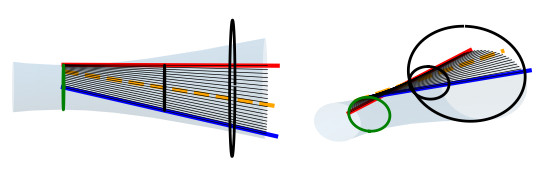
\includegraphics[width=12cm]{figures/npa_intersection.jpg}
    \caption{Two views of a (exaggerated) Gyro-surface (light blue) created by fast-neutral trajectories. The two black rings are the aperture (smaller circle) and the detector (larger circle). The green circle is the gyro-ring. The red/blue lines shows the first/last trajectory to pass through the aperture and hit the detector. The dashed orange line shows the representative trajectory used for the collisional radiative model. The thin black lines shows the trajectories over which the neutral flux is distributed.}
    \label{fig:npa_intersect}
\end{figure}

The initial population flux is the same as Equation \ref{eq:fast_rates} with the $N_f/N_t$ term replaced with $w_i\Delta\gamma/2\pi$. Since the path length of the trajectories within the gyro-range are similar, the collisional radiative model is only calculated for the middle trajectory. The neutral flux is then equally distributed among the other trajectories in the range. This is done so that the particles that hit the detector are not biased towards the center of the detector. This approach also drastically sped up the NPA calculation and is now comparable to the FIDA calculation. It is also equivalent with the previously discussed method. Figure \ref{fig:npa_flux} compares the solid angle approach with the gyro-angle approach. Both methods give the same neutral flux.
\begin{figure}[h!]
    \centering
    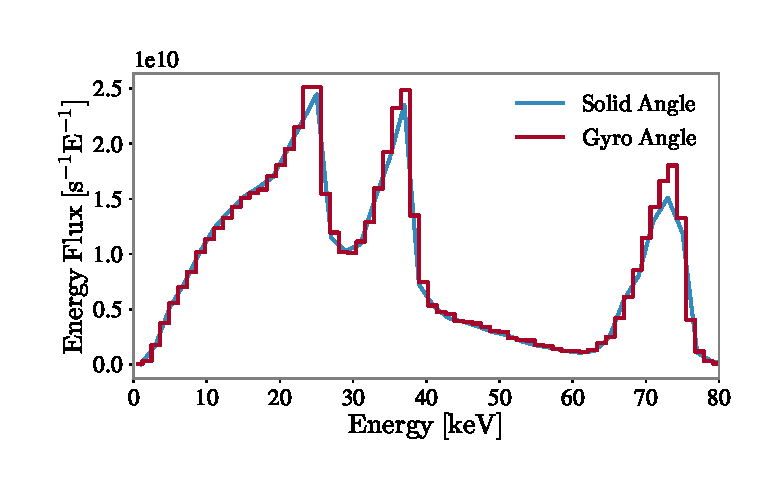
\includegraphics[width=13cm]{figures/inpa_flux.eps}
    \caption{Incident energy flux for imaging NPA: Solid angle NPA calculation (blue) and the Gyro Angle approach (red step). Both methods give the same energy flux.}
    \label{fig:npa_flux}
\end{figure}

\section{Simulation of Beam-Plasma Neutron Rates}
A recent addition to FIDASIM is the ability to calculate volume-averaged beam-plasma neutron rates. Because there are no geometric effects to consider, the calculation of the neutron rate is straight forward and is given by
\begin{equation}\label{eq:neutron_rate_f}
    \rm{rate} = \iiiint F(E,p,R,Z) \int_0^{2\pi} S_{neutron}(E,p,R,Z,\gamma) \,d\gamma\,dE\,dp\,dR\,dZ\,,
\end{equation}
where $S_{neutron}$ is the forward model of the neutron detector specified in Equation \ref{eq:W_neutron} and $F(E,p,R,Z)$ is the guiding center fast-ion distribution function.
If a guiding center Monte Carlo distribution was used, the neutron rate would be given by
\begin{equation}\label{eq:neutron_rate_gcmc}
    \rm{rate} = \sum_i^{N_p}\left (\frac{w_i}{2\pi} \int_0^{2\pi}  S_{neutron}(E_i,p_i,R_i,Z_i,\gamma) \,d\gamma \right )\,,
\end{equation}
where $w_i$ is the weight of the Monte Carlo particle such that the total number of fast ions is given by $\sum_i^{N_p} w_i$. If a full orbit Monte Carlo distribution is used, the neutron rate is given simply by
\begin{equation}\label{eq:neutron_rate_fomc}
    \rm{rate} = \sum_i^{N_p}\left (w_i S_{neutron}({v_r}_i,{v_\phi}_i,{v_z}_i,R_i,Z_i,\phi_i) \right ).
\end{equation}
From the above equations, it is plain to see that the neutron rate is just the sum of the rates from the individual fast-ions. In the next chapter, we will see that all the discussed diagnostics can be expressed in a similar manner.
\chapter{Fast-ion Diagnostic Weight Functions}\label{chap:weights}

From a diagnostics standpoint, fast-ion physics is particularly difficult.
Unlike bulk-ion diagnostics that measure Maxwellian distributed velocities, fast-ion diagnostics  measure a velocity distribution that can be highly anisotropic due to neutral beam and RF heating.
The lack of a simple parametrization of the fast-ion velocity distribution makes it difficult to draw correlations between experimental data and the relevant fast-ion physics.
In an effort to aid the modeling, interpretation, and experimental design of fast-ion diagnostics, the following \textit{ansatz} was proposed\cite{heidbrink2007}
\begin{equation}\label{eq:vs_WF}
    S_{tot} = \iint W(E,p)F(E,p)\,dEdp\,,
\end{equation}
where $S_{tot}$ is the total diagnostic signal, $F(E,p)$ is the fast-ion energy-pitch distribution function, and $W(E,p)$ is a diagnostic weighting function, colloquially known as the velocity-space weight function. The weight function indicates the phase-space sensitivity of the diagnostic, allowing for easier interpretation of the diagnostic data. As an aside, it is also common to formulate the weight functions in terms of the velocities parallel and perpendicular to the magnetic field, hence the name velocity-space weight functions. The transformation between the two coordinates is detailed in Appendix \ref{app:ep2vs}.

In the following sections, we will discuss how velocity-space weight functions are used and their limitations. We then show how to derive generalized diagnostic weight functions from the full forward models. With this firm theoretical footing, we also show how the generalized weight functions can be used to derive weight functions in guiding-center orbit space.

\section{Velocity-space Weight Functions}
Since their introduction, there has been a focused effort in calculating velocity-space weight functions for fast-ion diagnostics\cite{salewski2011,salewski2014,jacobsen2015,salewski2015,salewski2016}. Figure \ref{fig:vs_weights} shows velocity-space weight functions, calculated by FIDASIM, for the neutron, NPA, and FIDA diagnostics. The velocity-space weight functions are used primarily to interpret diagnostic signals. While forward modeling can tell you \textit{what} the expected diagnostic signal should be, it provides little insight into the \textit{why}. Velocity-space weight functions provide a way to inspect diagnostic signals at a deeper level. 
\begin{figure}[ht]
    \centering
    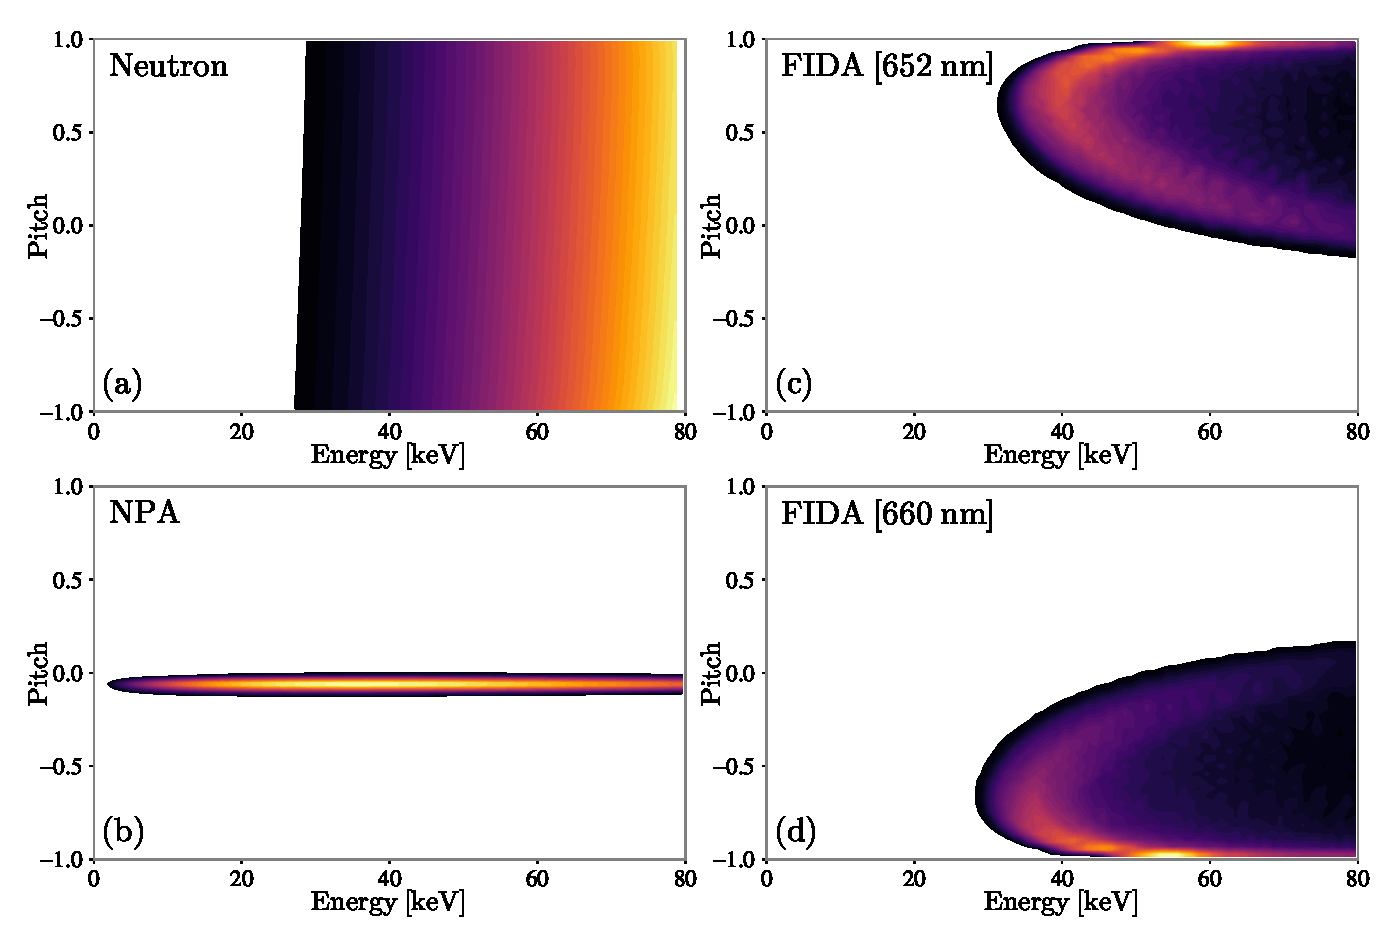
\includegraphics[width=13cm]{figures/velocity_space_weights.eps}
    \caption{Representative velocity-space weight functions for the DIII-D plasma and diagnostics. (a) The neutron scintillator is a global measurement of the neutron production rate. Its weight function for beam-plasma neutron production is spatially averaged and shows a strong energy dependence. The slight anisotropy in pitch is due to fast ions traveling with (positive pitch) and against (negative pitch) the plasma rotation. (b) The Neutral Particle Analyzer (NPA) diagnostic detects neutralized fast ions that escape the plasma. The collimation of the detector only permits a small range of pitch values to hit the detector and, because the detector is operated in current mode, the weight function is sensitive to many different energies. (c-d) The Fast-ion Deuterium-$\alpha$ (FIDA) diagnostic measures spectra produced by neutralized fast ions. The weight function 
depends upon wavelength. These FIDA weight functions are line-of-sight 
averaged at $\lambda = (652,660) \pm 0.2 \;\rm{nm}$ for a single oblique (Fig. \ref{fig:geometry}) viewing chord.}
    \label{fig:vs_weights}
\end{figure}

For instance, in an experiment at DIII-D, a modulated low power neutral beam was used to create an oscillating fast-ion population. The shot (\#157725) had minimal magneto-hydrodynamic (MHD) instabilities and was intended to be a baseline for later discharges. A radial array of FIDA chords---the oblique system in Fig. \ref{fig:geometry}---was used to monitor the oscillating fast-ion population. Figure \ref{fig:fida_waveform} shows FIDA waveforms conditionally averaged over four 54ms oscillation periods for the different radial positions. Figures \ref{fig:fida_waveform_low} and \ref{fig:fida_waveform_high} show the waveforms for data integrated over small and large Doppler shifts respectively. 
\begin{figure}[ht]
    \centering
    \subfigure[][]{%
        \label{fig:fida_waveform_low}
        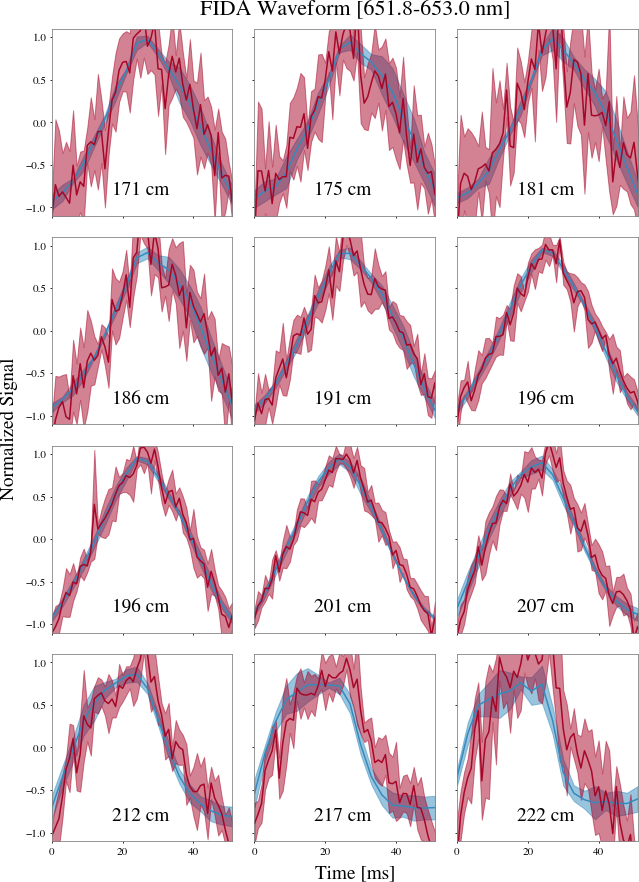
\includegraphics[width=7cm]{figures/FIDA_waveform_21_40_kev.png}}
    \hspace{2pt}
    \subfigure[][]{
        \label{fig:fida_waveform_high}
        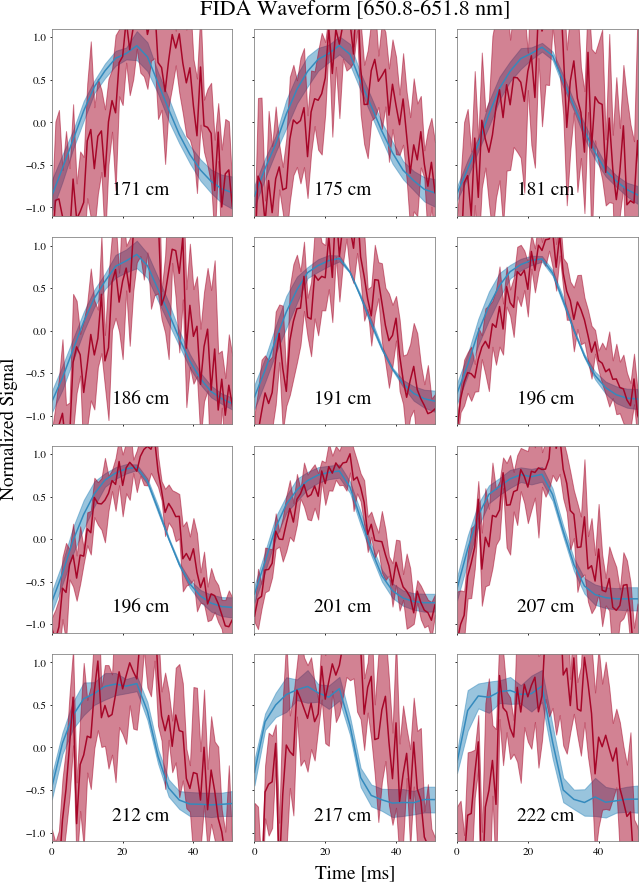
\includegraphics[width=7cm]{figures/FIDA_waveform_40_61_kev.png}}
    \caption{FIDA waveforms for DIII-D shot \#157725 for two different integration ranges:
        \subref{fig:fida_waveform_low} Small Doppler shift/alpha waveform: $\Delta \lambda = 651.8-653.0\;nm$;
        \subref{fig:fida_waveform_high} Large Doppler shift/beta waveform: $\Delta \lambda = 650.8-651.8\;nm$.
        FIDA data and error-bars averaged over four oscillation periods are shown in red, the corresponding weight function calculated theoretical signals are shown in blue. Errors in the theoretical signals derive from varying plasma profiles over the different periods. The neutral beam is on during the first half of the period and off during the second half.}
    \label{fig:fida_waveform}
\end{figure}

Despite looking at the same radial location, the waveforms for the small and large Doppler shifts, which will henceforth be called the alpha and beta waveforms respectively, are different. In the core region ($\sim181$ cm), the alpha waveform slowly increases in the first half of the period, when the beam is on, and slowly decays in the second half, when the beam is off. The beta waveform shows the opposite trend: growing quickly when the beam is on and decaying quickly when it is turned off. Forward modeling alone is unable to explain the different trends. Velocity-space weight functions, however, allows us to determine where in velocity-space the signal is originating. Figure \ref{fig:fida_waveform_WF} compares the waveforms at $R=181$ cm and shows the corresponding time evolution of the products of the velocity-space weight functions and the local theoretical distribution, $W(E,p)\times F(E,p)$.
\begin{figure}[h!]
    \centering
    \includegraphics[width=15cm]{figures/FIDA_waveform_compare.eps}
    \caption{Weight function analysis: Top row: comparison of the FIDA waveforms for small/alpha (red line) and large/beta (blue line) Doppler shifts at $R=181$ cm. Colored dashed lines are the data. Middle row: time evolution of the product of the large Doppler shift velocity-space weight function and the local theoretical distribution function. Bottom row: time evolution of the product of the small Doppler shift velocity-space weight function and the distribution function. The color-maps increase linearly from light to dark. The distribution function is calculated using the TRANSP/NUBEAM\cite{NUBEAM} code.}
    \label{fig:fida_waveform_WF}
\end{figure}
The weight functions in Figure \ref{fig:fida_waveform_WF} are sensitive to different regions in phase-space. The alpha weight function is only sensitive to fast ions with energies greater than $\sim$40keV, while the beta weight function is sensitive to lower energies, $>$20keV. If we take the weight functions to have a similar pattern of sensitivity as Figure \ref{fig:vs_weights}c, the reasons for the shape of the waveforms are apparent. For the beta waveform, the fast-ions are born into a higher sensitivity region and move into regions of zero sensitivity. Comparatively, for the alpha waveform the fast ions are born in a low sensitivity region and move into higher sensitivity regions as they slow down. This results in a quicker growth in the beta waveform and slower growth in the alpha waveform. When the beam is turned off in the middle of the period, the alpha waveform decays slowly due to a large fraction of the fast-ions still in the weight function's sensitive region. For similar yet opposing reasons, the beta waveform decays more quickly when the beam is turned off.

In addition to enhancing our ability to analyze experimental data, velocity-space weight functions provide a method of inferring the local fast-ion distribution function\cite{salewski2013_tomography,salewski2014_tomography}. Equation \ref{eq:vs_WF} can be discretized, creating a system of linear equations. When multiple diagnostics view the same spatial location, the system of linear equations can be solved via various numerical methods\cite{jacobsen_stagner2016}. This application of weight functions will be discussed, in depth, in the next chapter.

Velocity-space weight functions have enhanced our ability to understand diagnostic signals and, through Velocity-space Tomography, the fast-ion distribution function itself. However, velocity-space weight functions are hindered, both in their accuracy and in their practicality due to the implicit assumption that diagnostic signals are spatially localized. The flaws in this assumption can be made plain by comparing the diagnostic signals calculated using FIDASIM and Equation \ref{eq:vs_WF}.
\begin{figure}[h!]
    \centering
    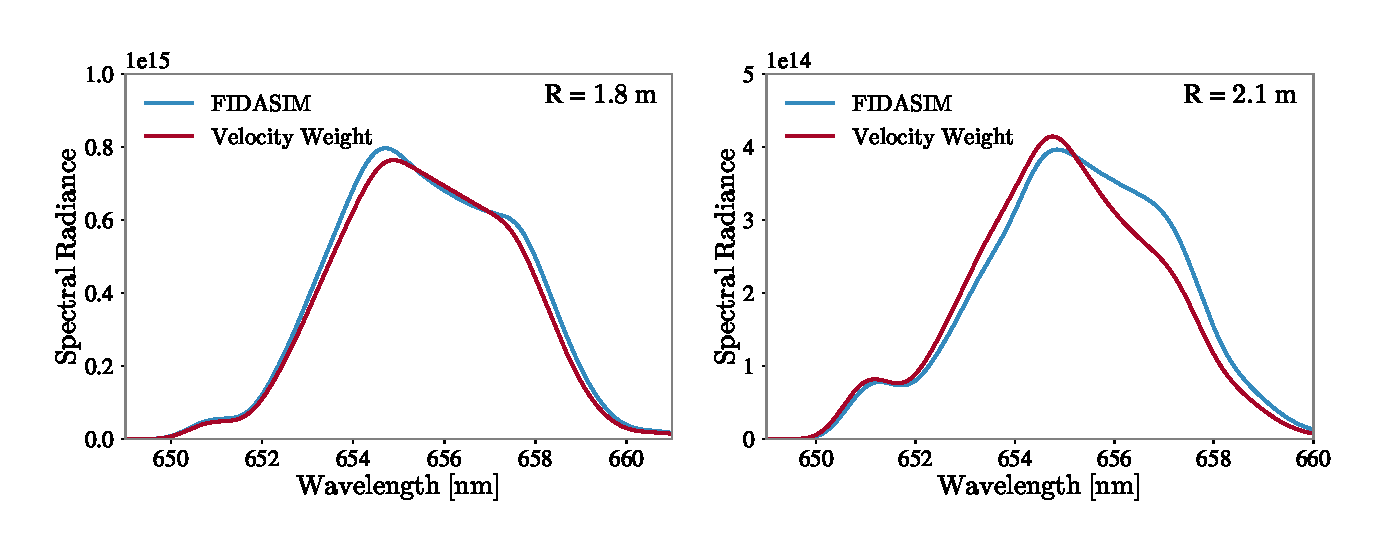
\includegraphics[width=15cm]{figures/fida_spectra.eps}
    \caption{FIDA spectra calculated using velocity-space weight functions 
(Equation~\ref{eq:vs_WF}) for the oblique viewing chords at
(a) $R = 1.8$ and (b) $R = 2.1$ m.  The spectra calculated by FIDASIM are also shown.
 Disagreement between FIDASIM and Equation \ref{eq:vs_WF} is because the latter uses a local fast-ion distribution to calculate the spectra. Differences between the local distribution and the full distribution used by FIDASIM cause the two methods to disagree to varying degrees.}
    \label{fig:fida_spectra}
\end{figure}
In regions where the fast-ion distribution has large spatial variations, velocity-space weight functions perform poorly.
Figure~\ref{fig:fida_spectra} shows spectra calculated using spatially-averaged velocity-space
weight functions.  Near the magnetic axis (Fig.~\ref{fig:fida_spectra}a), the calculated
spectrum agrees fairly well with FIDASIM, indicating that the velocity-space weight function method is fairly accurate. However,
off-axis (Fig.~\ref{fig:fida_spectra}b), the spectrum calculated with
velocity-space weight functions deviates significantly from FIDASIM.  Comparisons with simulations that use an uniform fast-ion distribution are not discrepant, showing that spatial variations are responsible for the deviation.
Generally, as in Figure \ref{fig:fida_spectra}, velocity-space weight functions agree with FIDASIM in the core, where spatial gradients are relatively smaller, than in the periphery, where variations in the fast-ion density and other quantities tend to be large.
This trend is also seen in Figure \ref{fig:fida_waveform}.

Another mark against velocity-space weight functions is that velocity-space tomography requires overlapping diagnostic views.
In practice, due to limited port access, radial arrays from one or two ports are more common than multiple views of the same spatial volume from different viewing locations. 
To resolve these crippling limitations, a generalization of Equation \ref{eq:vs_WF} to include spatial dependencies needs to be derived.

\section{Generalized Diagnostic Weight Functions} \label{sec:generalized_weight}
Velocity-space weight functions are typically derived using variations of probabilistic arguments\cite{salewski2011,salewski2014,jacobsen2015,salewski2015,salewski2015}. When considering a fixed location within the plasma, a probabilistic approach is often simpler. However, in order to properly account for the spatial dependencies of the diagnostics, a different tack is needed.

Consider a fast ion with phase-space coordinates $\mathbf{x} = [\mathbf{p},\mathbf{q}]$, where $\mathbf{p}$ and $\mathbf{q}$ are the generalized momentum and position, respectively.
As seen in Chapter \ref{chap:diagnostics}, the forward models for many fast-ion diagnostics can be expressed as a function, $S(\mathbf{x})$, which gives the expected signal produced by a fast ion with phase-space coordinates $\mathbf{x}$.
The total diagnostic signal is found by summing the contributions of all the individual fast ions,
\begin{equation}\label{eq:sum_S}
    S_{tot} = \sum_{k=1}^N S(\mathbf{x}_k),
\end{equation}
where $N$ is the total number of fast ions in the plasma.
This equation can be expressed in terms of the frequency in which $\mathbf{x}$ occurs
\begin{equation}\label{eq:sum_SP}
    S_{tot} = N \sum_{\mathbf{x}_k \in R_{X}} S(\mathbf{x}_k) P_X(\mathbf{x}_k),
\end{equation}
where $P_X(\mathbf{x}_k)$ is the frequency of $\mathbf{x}_k$ occurring.
In the continuum limit, the discrete sum in the above equation can be replaced by an integral and can be written in the form
\begin{equation}\label{eq:SF}
    S_{tot} = \int S(\mathbf{x})\,N \sum_{\mathbf{x}_k \in R_{X}} P_X(\mathbf{x}_k) \delta(\mathbf{x} - \mathbf{x}_k) d\mathbf{x} = \int S(\mathbf{x}) F(\mathbf{x}) d\mathbf{x},
\end{equation}
where $F(\mathbf{x})$ is the fast-ion distribution function.
By inspection, it is clear that Equation \ref{eq:SF} is the generalized version of equation \ref{eq:vs_WF}.

Upon comparing Equation \ref{eq:SF} with how FIDASIM simulates the diagnostics, it is apparent that they are equivalent as FIDASIM evaluates Equation \ref{eq:SF} via Monte Carlo integration.
\begin{equation}
    S_{tot} \approx \frac{1}{N_t} \sum_i^{N_t} S(\mathbf{x}_i)\quad \rm{where}\; \mathbf{x}_i \sim F(\mathbf{x})\,,
\end{equation}
where $N_t$ is the number of FIDASIM's ``trajectories'', which just correspond to samples, $\mathbf{x}_i$, from the distribution function, $F(\mathbf{x})$. In fact, FIDASIM's neutral density calculations can also put into the form of Equation \ref{eq:SF} where, instead of the fast-ion distribution, the distribution function is either the neutral beam distribution, for the beam density calculation, or the thermal ion distribution, for the direct charge exchange and halo densities.

From the generalized form, we can also derive the velocity-space weight functions.
Consider the phase-space coordinate system $\mathbf{x} = \{E,p,\gamma, R, Z, \phi\}$, where $E$ is the energy, $p$ is the pitch with respect to the plasma current ($p=v_{\parallel}/v$), $\gamma$ is the gyro-angle, $R$ is the major radius, $Z$ is the elevation, and $\phi$ is the toroidal angle. The velocity-space weight function in Equation \ref{eq:vs_WF} can be recovered by averaging over the phase-space variables $R$, $Z$, $\phi$, and $\gamma$.\footnote{To remind readers, averaging over a variable in a function involves integrating over the product of the function and the probability of the variable. For example, $g(x) = \int f(x,y)p(y)dy$ is averaging $f(x,y)$ over $y$.}
Since most velocity-space weight functions are gyro-averaged and spatially localized, the following reduction of equation \ref{eq:SF} reproduces the velocity-space weight function:
\begin{equation}\label{eq:vs_reduction}
    W(E,p) = \frac{1}{2\pi} \iiiint S(E,p,\gamma,R,z,\phi)\delta(R-R_0)\delta(z-z_0)\delta(\phi - \phi_0)\,d\gamma\, dR\, dz\, d\phi.
\end{equation}
At this point, we come to a clear understanding of what a velocity-space weight function actually is: a velocity-space weight function is the average signal produced by a fast ion with a given energy and pitch. 

\section{Orbit Weight Functions}\label{sec:orbit_weight}
A reduction of the phase-space, as done in Equation \ref{eq:vs_reduction}, greatly simplifies analysis and facilitates tomographic reconstructions by reducing the number of unknown parameters.
However, since we are concerned about the motion of the fast ions, care must be taken to ensure that no critical information is lost when averaging over variables.
In other words, only variables that do not appear in the Lagrangian (i.e. ignorable or cyclic coordinates) can be averaged out without critical information loss.
By this standard, the phase-space reduction done in Equation \ref{eq:vs_reduction} is inadequate since only the gyro and toroidal angle averaging was permissible. 

In order to reduce the phase-space as much as possible without sacrificing model fidelity, it is advantageous to express the expected diagnostic signal, $S$, in canonical action-angle coordinates, $\mathbf{x} = (\mathbf{J},\mathbf{\Theta})$.
Action-angle coordinates are a set of canonical coordinates with the special property that the action variables, $\mathbf{J}$, are invariants of the motion and the angle coordinates, $\mathbf{\Theta}$, are cyclic/ignorable and can, therefore, be safely averaged over when reducing the phase-space. 
In these coordinates, information preserving phase-space reductions can then be succinctly expressed as
\begin{equation}\label{eq:action_angle_reduction}
    W(\mathbf{J}) = \left( \prod_i \frac{1}{\tau_i} \right) \int_0^{\tau_1}\ldots\int_0^{\tau_i} S(\mathbf{J},\mathbf{\Theta})\, d\mathbf{\Theta}\,,
\end{equation}
where $\tau_i$ are the periods of the angle coordinates and $W(\mathbf{J})$ is the action-space weight functions which is interpreted to be the average signal produced by a fast ion with action coordinates $\mathbf{J}$, similar to the velocity-space weight functions. 

The total diagnostic signal can be calculated using these action-space weight functions. Consider the subset of fast ions in a plasma with action coordinates, $\mathbf{J}_k$.
The signal produced by these fast ions is given by
\begin{equation}\label{eq:orbit_tomography_discrete}
    S_k = \sum_i^{N_k} S(\mathbf{J}_k,\mathbf{\Theta}_i) = N_k \sum_i^{N_k} S(\mathbf{J}_k,\mathbf{\Theta}_i)/N_k\,,
\end{equation}
where $N_k$ is the number of fast ions with action coordinates $\mathbf{J}_k$.
The sum on the right-hand side is the average signal produced by the subset of fast ions. This is identical to the interpretation of the action-space weight function.
The total diagnostic signal can then be expressed as a linear combination of weight functions,
\begin{equation}\label{eq:orbit_tomography}
    S_{tot} = \sum_k N_k W(\mathbf{J}_k) .
\end{equation}
In the context of guiding center motion, $\mathbf{J}_k$ acts as a label for an individual fast-ion orbit. Therefore, Equation \ref{eq:orbit_tomography} can be interpreted as a sum of the signal produced by each fast-ion orbit.
As in velocity-space tomography, when there are multiple measurements, Equation \ref{eq:orbit_tomography} can be put into matrix form, creating a system of linear equations that can be solved. This is discussed in Chapter \ref{chap:orbit_tomography}.

An action-angle parametrization of the guiding center motion of a fast ion in a tokamak has three action coordinates and three angle coordinates.
There are many possible choices for action-angle coordinates; the classical choice being the canonical constants of motion: energy, magnetic moment, and toroidal canonical angular momentum, $\mathbf{J} = (E,\mu,p_\phi)$.
However, due to an ambiguity in the sign of $v_\parallel$ in the definition of $p_\phi$, the classical choice of coordinates does not always \textit{uniquely} label distinct orbits, i.e. a single action coordinate $ \mathbf{J}_k$ in this space could correspond to two different orbit trajectories (orbit degeneracy). This can be plainly seen by expressing the magnetic moment as a function of the energy and toroidal angular momentum. 
\begin{equation}\label{eq:mu}
\mu(R,Z) = \frac{E}{B(R,Z)} - \frac{B(R,Z)}{2m} \left ( \frac{p_\phi - q\Psi(R,Z)}{RB_\phi(R,Z)}\right)^2
\end{equation}
Isolines of this function are the orbit trajectories for a fixed $\mu$, $E$ and $p_\phi$.
\begin{figure}[h!]
    \centering
    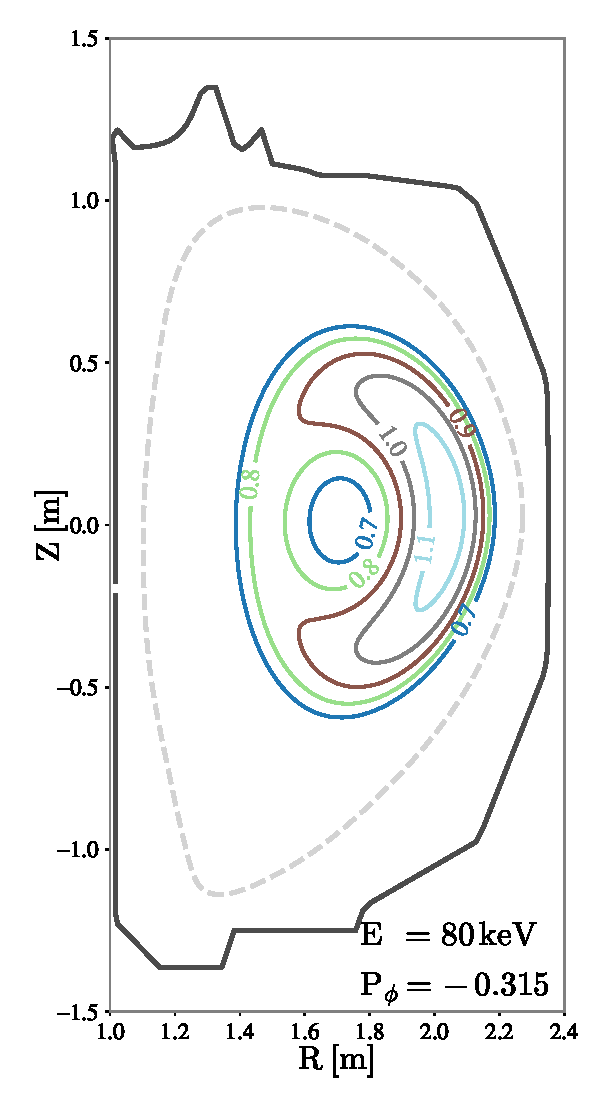
\includegraphics[width=7cm]{figures/hamiltonian_orbits.eps}
    \caption{Orbit trajectories generated by a scan of normalized magnetic moments, fixing energy (80 keV) and normalized canonical angular momentum (-0.315). Orbits are labeled by their normalized magnetic moments. Orbits with normalized magnetic moments of 0.7 and 0.8 are degenerate.}
    \label{fig:hamiltonian_orbits}
\end{figure}
Figure \ref{fig:hamiltonian_orbits} shows a scan over $\mu$ for a fixed $E$ and $p_\phi$. The scans show distinct orbits that have the same Hamiltonian coordinates.
The large distance between the orbits indicate that their fast-ion populations are independent and should be treated separately.
Orbit degeneracy also makes it impossible to use Equation \ref{eq:action_angle_reduction} to reduce the phase-space since the angle variables of the two orbits would have different periods.

To avoid this problem, we use a modified version of the coordinates first promoted by Rome\cite{rome1979} and others\cite{petrov2016}.
Here we define the action coordinates, hereby called orbit-space coordinates, to be
\begin{equation}\label{eq:orbit_action}
    \mathbf{J} = (E, p_m, R_m)\,,
\end{equation}
where $E$ is the energy, $R_m$ is the maximal radius along the orbit, and $p_m$ is the pitch with respect to the plasma current at $R_m$.
The angle variables, which describe the position of the fast ion along the orbit, are
\begin{equation}\label{eq:orbit_angle}
    \mathbf{\Theta} = (t, \gamma, \phi_0)\,,
\end{equation}
where $t$ is the time, $\gamma$ is the gyro-angle, and $\phi_0$ is the initial toroidal angle.
Applying Equation \ref{eq:action_angle_reduction} yields the definition of an orbit weight function,
\begin{equation}\label{eq:orbit_weight}
    W(E,p_m,R_{m}) = \frac{1}{4\pi^2 \tau_p}\int_0^{2\pi} \int_0^{2\pi} \int_0^{\tau_p} S(E,p_m,R_{m},t,\gamma,\phi_0)\,dt\, d\gamma d\phi_0\,,
\end{equation}
where $\tau_p$ is the poloidal transit time.

This choice of orbit-space coordinates has several nice properties. The space has natural boundaries in all three coordinates ($E = [0,E_{max}]$, $R_m = [R_{axis},R_{wall}]$, and $p_m = [-1,1]$),
 which makes it easy to enumerate all possible orbit trajectories for a given magnetic equilibrium.
Additionally, as can be seen in the topological map of the orbit-space in Fig. \ref{fig:orbit_topology}, counter-passing orbits are easily identified by the sign of $p_m$.
\begin{figure}[ht]
    \centering
    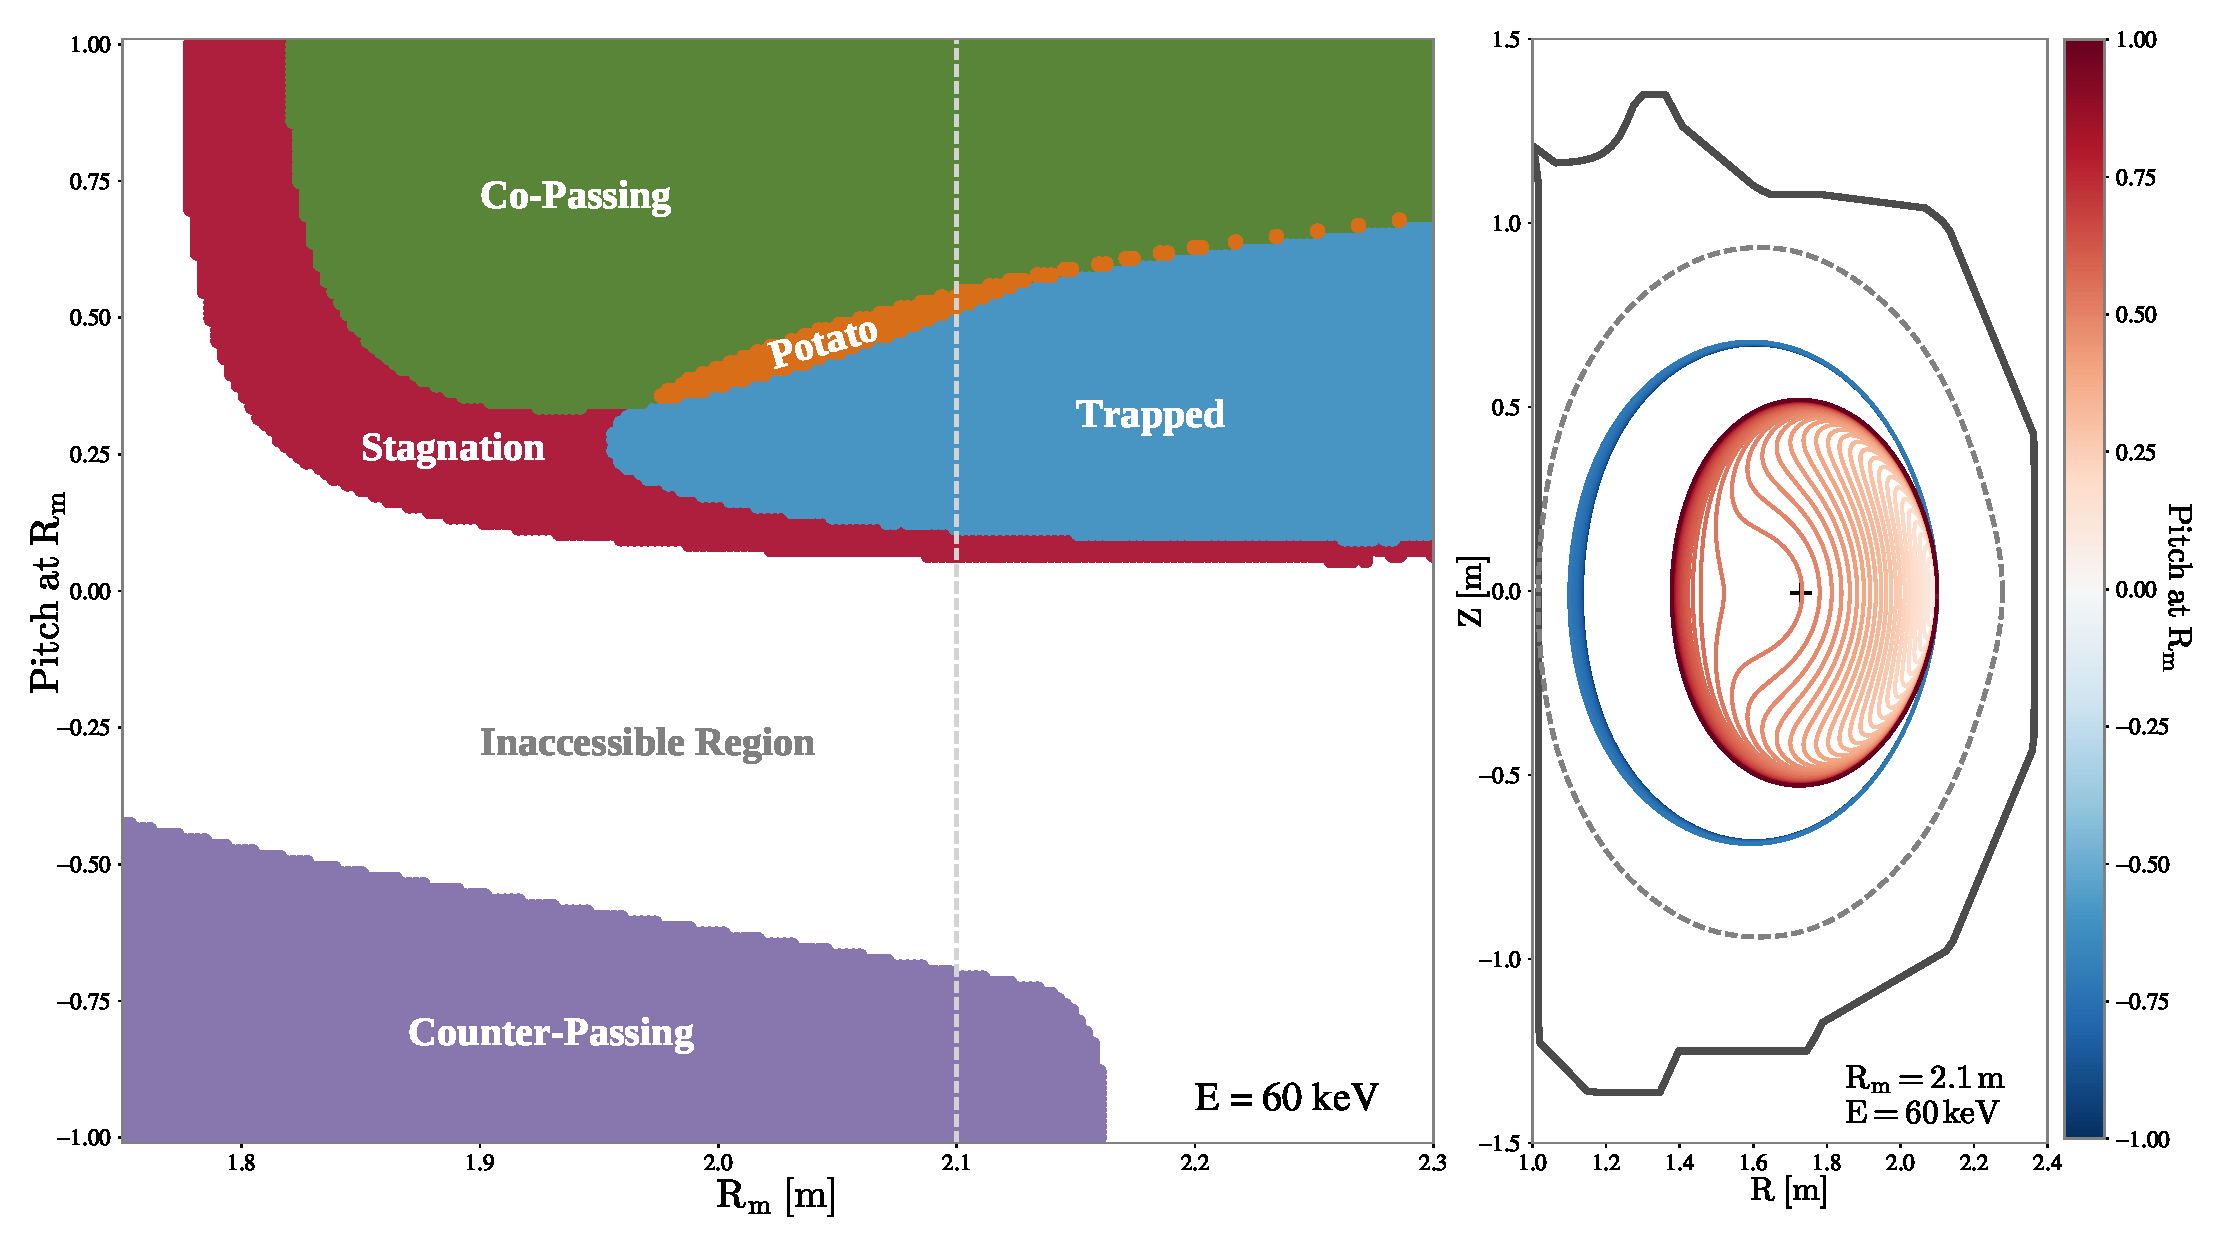
\includegraphics[width=15cm]{figures/orbit_topology3.eps}
    \caption{Left: Topological map of different orbit types \cite{WHITE} with fixed energy
for the DIII-D plasma described in Sec.~\ref{sec:apparatus}.
 \newline Right: Orbits corresponding to the dashed line in the topological map. The
plus indicates the magnetic axis and the dashed line is the last-closed flux surface. Counter-passing orbits have negative pitch along their orbit, while co-passing orbits have constant positive pitches. Stagnation orbits are co-passing orbits that do not enclose the magnetic axis. The pitches of fast ions on a trapped orbit change signs and potato orbits are trapped orbits that enclose the magnetic axis.}
    \label{fig:orbit_topology}
\end{figure}

\subsection{Numerical Calculation of Orbit Weight Functions}
As the name suggests, fast-ion orbits are needed to calculate orbit weight functions. The orbit trajectories are found by solving the guiding-center drift orbit ordinary differential equation given by
\begin{equation}\label{eq:gc_ode}
    \mathbf{v}_{GC} = \frac{v_{\parallel}\mathbf{B}}{|B|} + \mathbf{v}_{E \times B} + \mathbf{v}_{grad} + \mathbf{v}_{curv}\,,
\end{equation}
where $v_{\parallel}$ is the velocity parallel to the magnetic field $\mathbf{B}$ and the remaining terms are the $E\times B$, gradient, and curvature drifts respectively. Notice that unlike other guiding center orbit codes, the inclusion of the $E \times B$ drift is necessary.
\begin{figure}[h!]
    \centering
    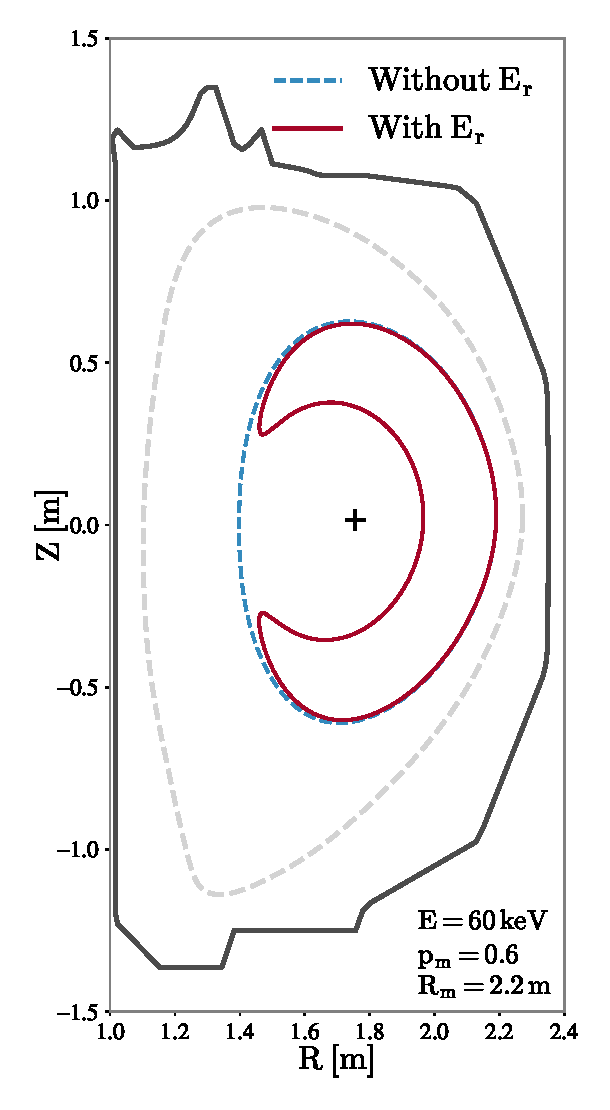
\includegraphics[width=7cm]{figures/orbit_er.eps}
    \caption{Two orbits, one including the effects of the radial electric field (red line), one without (blue dashed line). Including the radial electric field changes the orbit topology.}
    \label{fig:orbit_er}
\end{figure}
As shown in Figure \ref{fig:orbit_er}, including the effects of the radial electric field can substantially change the trajectory of the orbit and, consequentially, the orbit's weight function. For this reason, the $E \times B$ drift must be included.

The orbit coordinates, describe in the previous section, provide three out of the four initial conditions needed to solve Equation \ref{eq:gc_ode}: the kinetic energy, pitch, and $R$. The fourth initial condition is the initial $Z$ position of the fast-ion. The initial Z position is found by finding the point of minimum poloidal flux at a fixed value of major radius, $R_m$. Since fast-ions are mostly tied to a flux surface at the outermost legs of their orbits, the point of minimum flux is also a point on the orbit.

Once all the initial conditions are found, Equation \ref{eq:gc_ode} is solved for one poloidal transit time of the orbit, with particle locations and velocities dumped at equal time steps throughout the interval $[0,\tau_p)$. The particles are given equal weights and loaded into the diagnostic's forward model, e.g. FIDASIM---this is equivalent to evaluating the integral in Equation \ref{eq:orbit_weight}. Orbits that are degenerate or intersect the vessel wall have null orbit weights and are excluded.

The calculation of the orbit weights can be computationally intensive. To reduce the computational time, an orbit with small time steps can be down-sampled to an orbit with larger time steps. This reduces the number of particles used in the calculation. Using a down-sampling method, instead of using a larger time step when the orbit is first calculated, perseveres the accuracy of the orbit trajectory. Typically, the down-sampling time step is chosen such that the mean poloidal distance between particles is $\sim1$ cm. An example of a down-sampled orbit is shown in Figure \ref{fig:down_sample}.
\begin{figure}[h!]
    \centering
    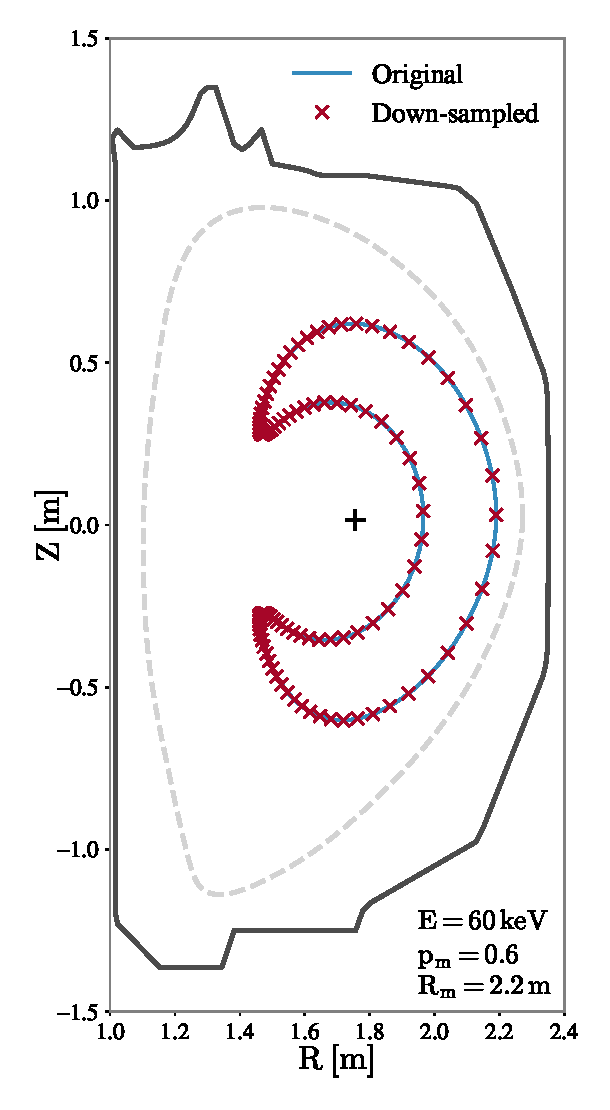
\includegraphics[width=7cm]{figures/down_sampled_orbit.eps}
    \caption{Example of a down-sampled orbit. The blue line is the original orbit and the red x's are the points used to calculate the orbit's weight function. For illustrative purposes, the mean poloidal length between points is set to 4 cm. Typically, a mean poloidal length of 1 cm is used.}
    \label{fig:down_sample}
\end{figure}

\subsection{Orbit Weight Functions for Various Fast-ion Diagnostics}
In this section, after briefly describing the plasma conditions and diagnostics,
orbit weight functions are calculated for three DIII-D fast-ion diagnostics: 
the neutron scintillator, the solid state neutral particle analyzer (ssNPA), and the fast-ion D-$\alpha$ (FIDA) spectrometer.
The orbit weight functions are calculated on a $100 \times 100 \times 100$ element 
$(E,p_m,R_m)$ grid.

\subsubsection{Apparatus} \label{sec:apparatus}
The selected plasma is 
DIII-D shot \#159243 at 790 ms. This discharge, which is discussed in detail in
 Ref. \cite{heidbrink2017}, is a reversed-shear plasma with toroidal field of 2.0 T and
plasma current of +0.8 MA (counter clockwise). The fast-ion population is created by
deuterium neutral beams of energy 70-81 keV that are injected in
both the co-current and counter-current directions. Although the discharge has extensive Alfv\'en
eigenmode activity, only the ``classical'' distribution function calculated by NUBEAM
\cite{NUBEAM} in the absence of wave-induced transport is considered here.
Projections of the orbit-space fast-ion distribution function for the shot are shown in 
Figure \ref{fig:distribution}.
\begin{figure}[ht]
    \centering
    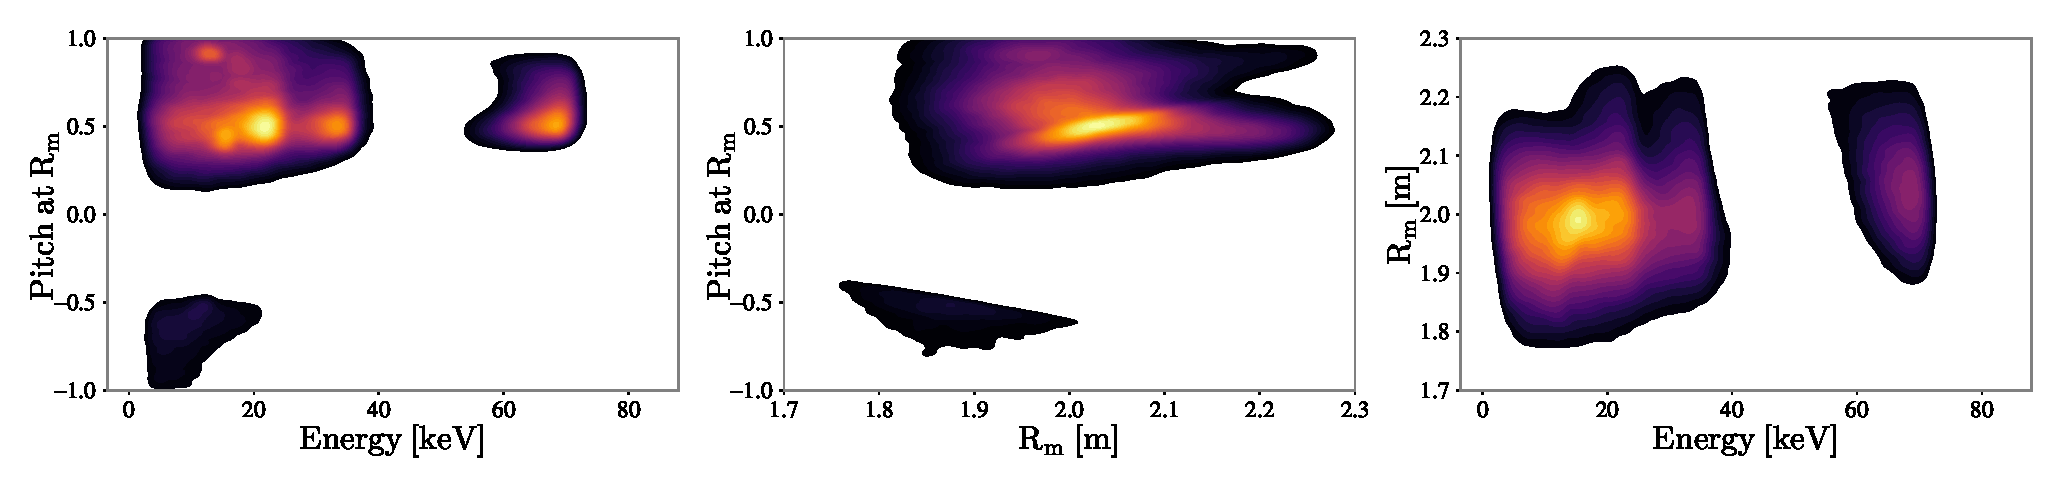
\includegraphics[width=15cm]{orbit_distribution}
    \caption{Projections of the orbit-space fast-ion distribution for shot \#159243 at 790 ms. Each projection is the full 3D distribution integrated over one of the variables, e.g. $F_z(x,y) = \int F(x,y,z)\;dz$.  Each projection is normalized to unity. The color-map increases linearly from dark(black) to light(yellow).}
    \label{fig:distribution}
\end{figure}


%==============================================================================
%---------------------------------- NEUTRON -----------------------------------
%==============================================================================

%\begin{figure}[ht]
%    \centering 
%    \includegraphics[width=15cm]{neutron_cross_section}
%    \caption{Energy dependence of neutron cross section for D-D fusion reactions.}
%    \label{fig:neutron_cross_section}
%\end{figure}
\subsubsection{Neutron Scintillator Orbit Weight Function}
The neutron scintillator measures the volume-averaged neutron rate; Figure \ref{fig:neutron_orbit_weight} shows its orbit weight function.
In isolation, the neutron orbit weight function gives insight into the underlying physics of the diagnostic.
\begin{figure}[h!]
    \centering
    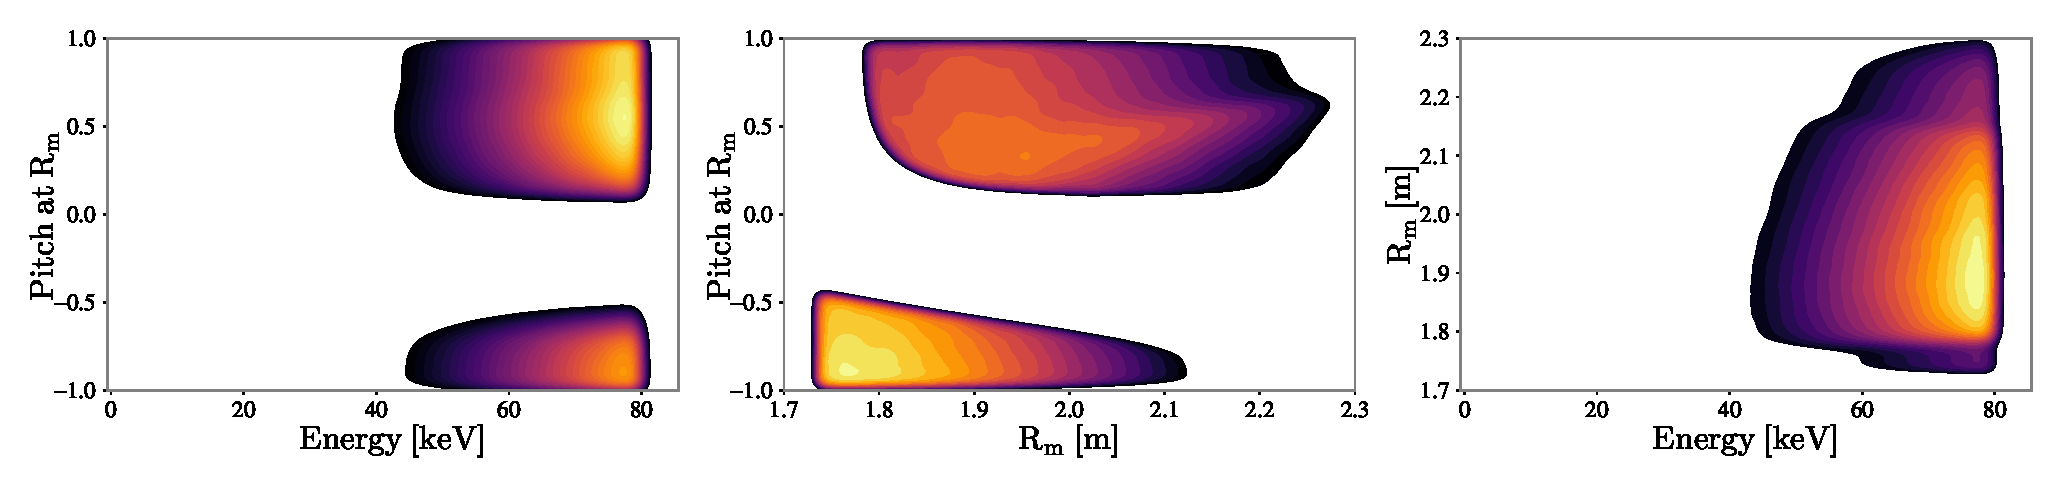
\includegraphics[width=17cm]{figures/neutron_orbit_weight.eps}
    \caption{Normalized projections of the 3D neutron orbit weight function.}
    \label{fig:neutron_orbit_weight}
\end{figure}
For example, the strong energy dependence of the orbit weight function indicates that the effect of the neutron cross section is considerable. This type of analysis can also be done using velocity-space weight functions; however, with orbit weights the sensitivity of the diagnostic to individual orbit types can also be analyzed.
\begin{table}[h!]
    \centering
    \begin{tabular}{|c|c|c|c|}
    \hline
    Orbit Type & Average Weight [$s^{-1}$] & Phase-space Fraction & Signal Produced [$s^{-1}$]\\
    \hline
    Potato      & $3.83\times10^{-5}$ & $7.75\times10^{-3}$ & $1.19\times10^{12}$  \\
    Stagnation  & $3.69\times10^{-5}$ & $9.61\times10^{-2}$ & $2.86\times10^{11}$  \\
    Trapped     & $2.09\times10^{-5}$ & $2.41\times10^{-1}$ & $5.65\times10^{12}$  \\
    Ctr-Passing & $2.82\times10^{-5}$ & $2.93\times10^{-1}$ & $3.67\times10^{11}$  \\
    Co-Passing  & $2.67\times10^{-5}$ & $3.62\times10^{-1}$ & $1.57\times10^{13}$  \\
    \hline
    Total       &                     &                     & $2.32\times10^{13}$  \\
    \hline
    \end{tabular}
    \caption{Dependence of neutron signal on orbit topology for DIII-D discharge \#159243 at 790 ms. Column~1: Type \cite{WHITE} of orbit. Column~2: Average neutron signal produced by a fast ion of the given type. Column~3: Fraction of the fast-ion phase space occupied by the orbit type. Column~4: Total neutron signal produced by each orbit type. The table indicates that the neutron diagnostic is most sensitive to potato orbits. Additionally, it shows that counter-passing orbits produce more signal on average than co-passing orbits due to counter-passing orbits traveling against the bulk plasma rotation, causing a higher relative energy. See the caption of Figure \ref{fig:orbit_topology} for explaination of the different orbit types.}
    \label{tab:neutron_orbit_weight}    
\end{table}
\begin{figure}[h!]
    \centering
    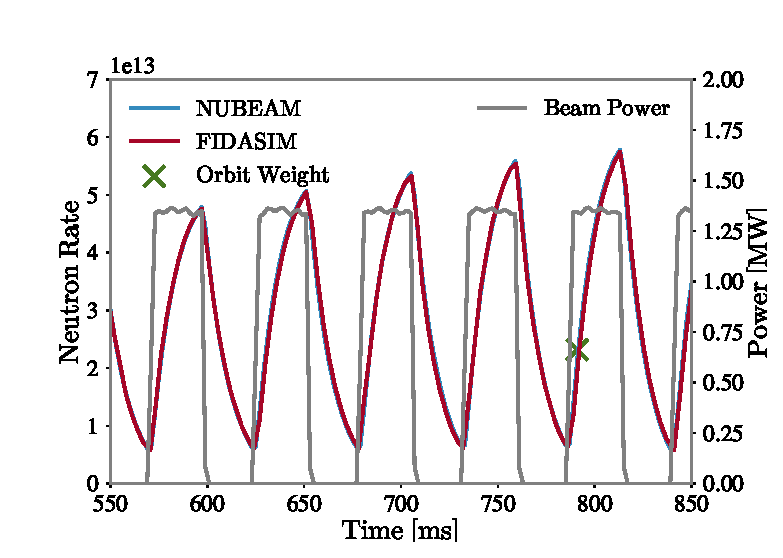
\includegraphics[width=10cm]{figures/neutron_rate.eps}
    \caption{Beam-plasma neutron rate and injected beam power over time for shot \#159243 calculated by the NUBEAM and FIDASIM codes and the rate at 790 ms calculated using the neutron orbit weight function and Equation \ref{eq:orbit_tomography}.}
    \label{fig:neutron_rate}
\end{figure}
Table \ref{tab:neutron_orbit_weight} shows the signal produced by each orbit type, indicating that co-passing orbits produce the most signal. Somewhat surprisingly, the neutron diagnostic is quite sensitive to potato orbits despite the small volume of phase space that they occupy. This is caused by the tendency of potato orbits to spend a large fraction of their orbit in the high density core region. 
The total beam-plasma neutrons produced, as calculated by Equation \ref{eq:orbit_tomography}, is in agreement with the predictions of TRANSP/NUBEAM and FIDASIM (Fig. \ref{fig:neutron_rate}).
\begin{figure}[h!]
    \centering
    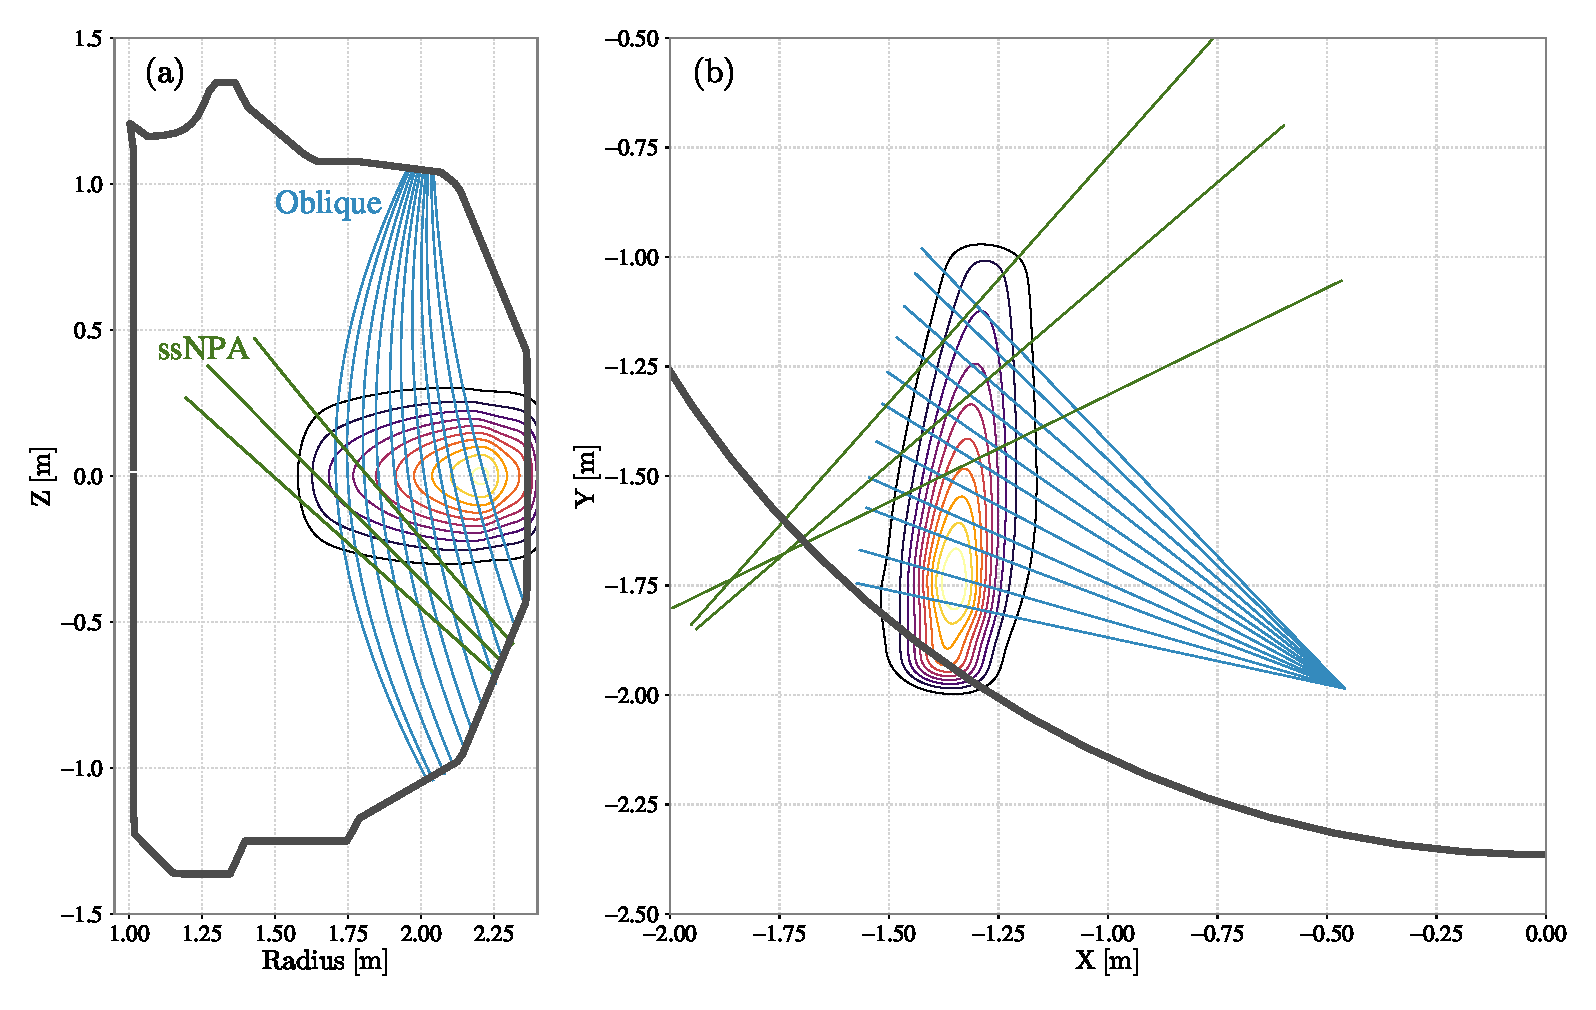
\includegraphics[width=15cm]{figures/geometry.eps}
    \caption{Poloidal (a) and plan (b) view of the 210RT neutral beam density (contours) and fast-ion diagnostics (colored lines). The Oblique FIDA system\cite{muscatello2010}, shown in blue, consists of of a maximum of 11 viewing chords looking down at the 210RT beam at an oblique angle of 
$\sim45^{\circ}$ with respect to the midplane. The solid state NPA system (ssNPA)\cite{ssNPA2012}, shown in green, consists of three channels viewing the core region of the plasma from below the midplane.}
    \label{fig:geometry}
\end{figure}

\subsubsection{NPA Orbit Weight Function}
The solid state NPA (ssNPA) diagnostic measures fast neutrals, born of charge exchange, that escape the plasma. DIII-D utilizes three separate channels, each viewing the 210RT neutral beam at a different radial location (Fig. \ref{fig:geometry}). In its present configuration, the detectors are operated in current mode \cite{ssNPA2012}.
Figure \ref{fig:npa_orbit_weight} shows the orbit weight function for the central channel. Upon inspection, it shows that the ssNPA diagnostic is localized in space ($R_m$) and in pitch ($p_m$), but, because the detector is operated in current mode, it is also sensitive to a large swath of energies. The localization in space and pitch is caused by the narrow collimation of the diagnostic. In a three dimensional view, the orbit weight function is characterized as a line through the orbit-space. As an aside, the previously discussed imaging NPA\cite{du2018inpa}, which is similarly localized in pitch but has an extended radial view, has an orbit weight function that takes the form of a 2d surface within the 3D orbit-space.
\begin{figure}[h!]
    \centering
    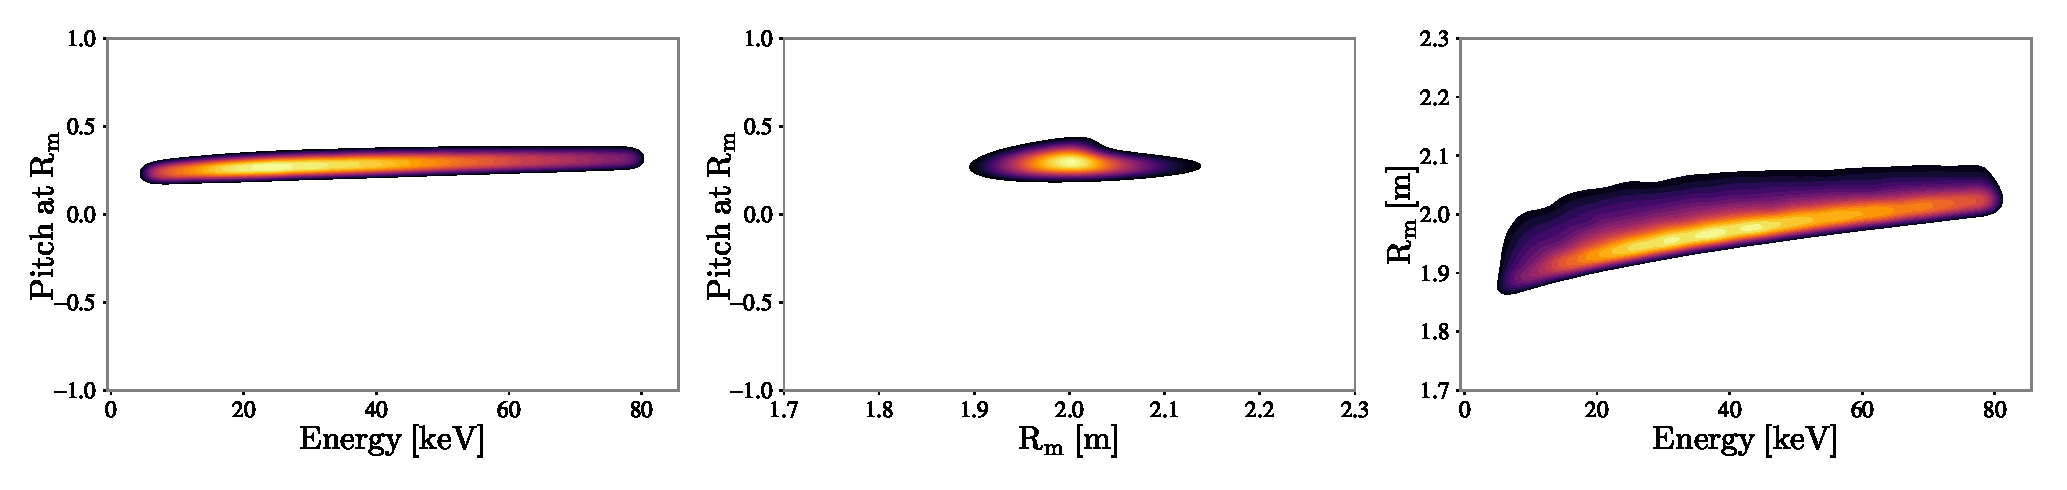
\includegraphics[width=15cm]{figures/npa_orbit_weight_2.eps}
    \caption{Normalized projections of the ssNPA(Fig. \ref{fig:geometry}) orbit weight function at R=1.64 m for shot \#159243 @ 790 ms}
    \label{fig:npa_orbit_weight}
\end{figure}

Providing further evidence that the orbit weight functions faithfully encode the ssNPA's full forward model, Figure \ref{fig:npa_ow_flux} shows that the energy resolved NPA flux calculated using the NPA orbit weights agrees with FIDASIM. 
\begin{figure}[h!]
    \centering
    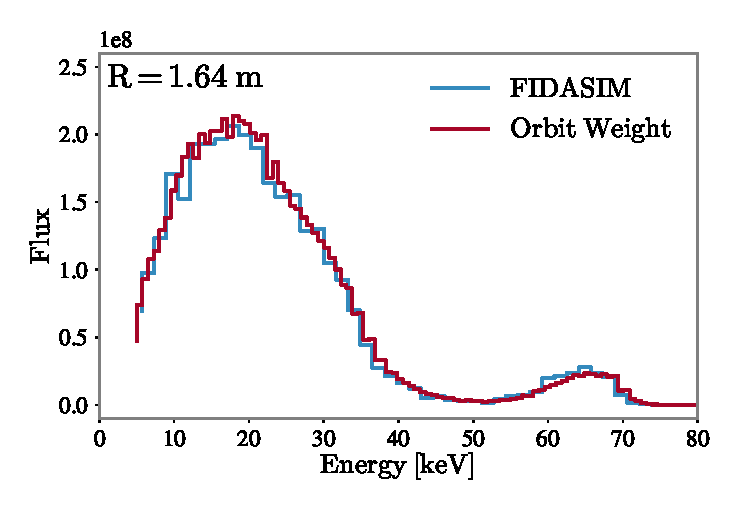
\includegraphics[width=10cm]{figures/npa_flux.eps}
    \caption{Comparison of the energy resolved ssNPA flux for shot \#159243 @ 790 ms calculated by FIDASIM and by the NPA orbit weight functions and Equation \ref{eq:orbit_tomography}.}
    \label{fig:npa_ow_flux}
\end{figure}

\subsubsection{Fast-ion D-$\alpha$ Spectroscopy (FIDA) Orbit Weight Function}
The main FIDA system used at DIII-D is the Oblique FIDA system (Fig. \ref{fig:geometry}), which consists of an array of radial views of the 210RT neutral beam.
The FIDA orbit weight functions depend on wavelength.
For instance, if we consider the orbit weight function for a red shifted wavelength (Fig. \ref{fig:fida_red}) we can see that the chord (oblique@1.9m) sees signal from counter-passing particles localized at $R_m$=1.91 m and also trapped particles from as far out as $R_m$=2.18 m. 
\begin{figure}[h!]
    \centering
    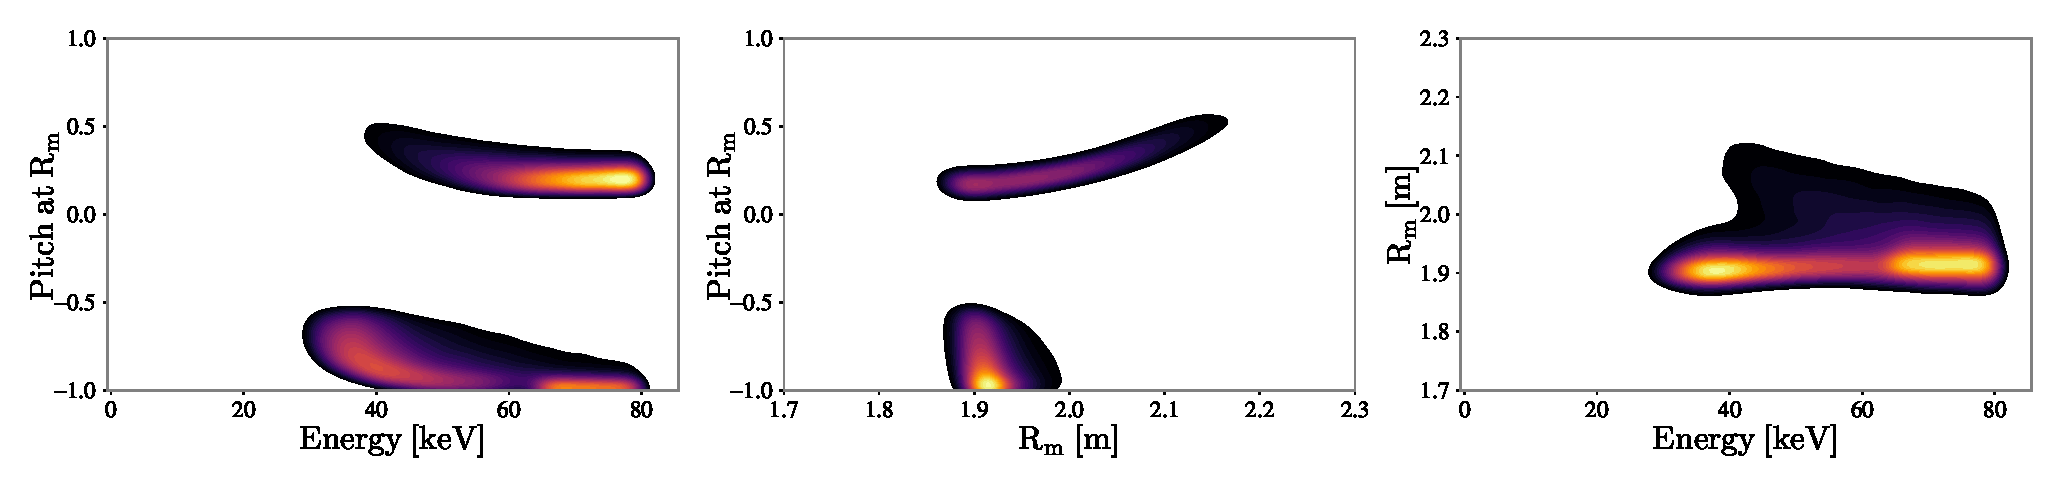
\includegraphics[width=15cm]{figures/fida_orbit_weight_red_14.eps}
    \caption{Projections of the red shifted ($\lambda = 660 \pm 0.2$ nm) FIDA orbit weight function for an oblique viewing chord with midplane intersection at R=1.9 m.}
    \label{fig:fida_red}
\end{figure}

We can also view the orbit weight function for a blue shifted wavelength for the same radial position (Fig. \ref{fig:fida_blue}). 
\begin{figure}[h!]
    \centering
    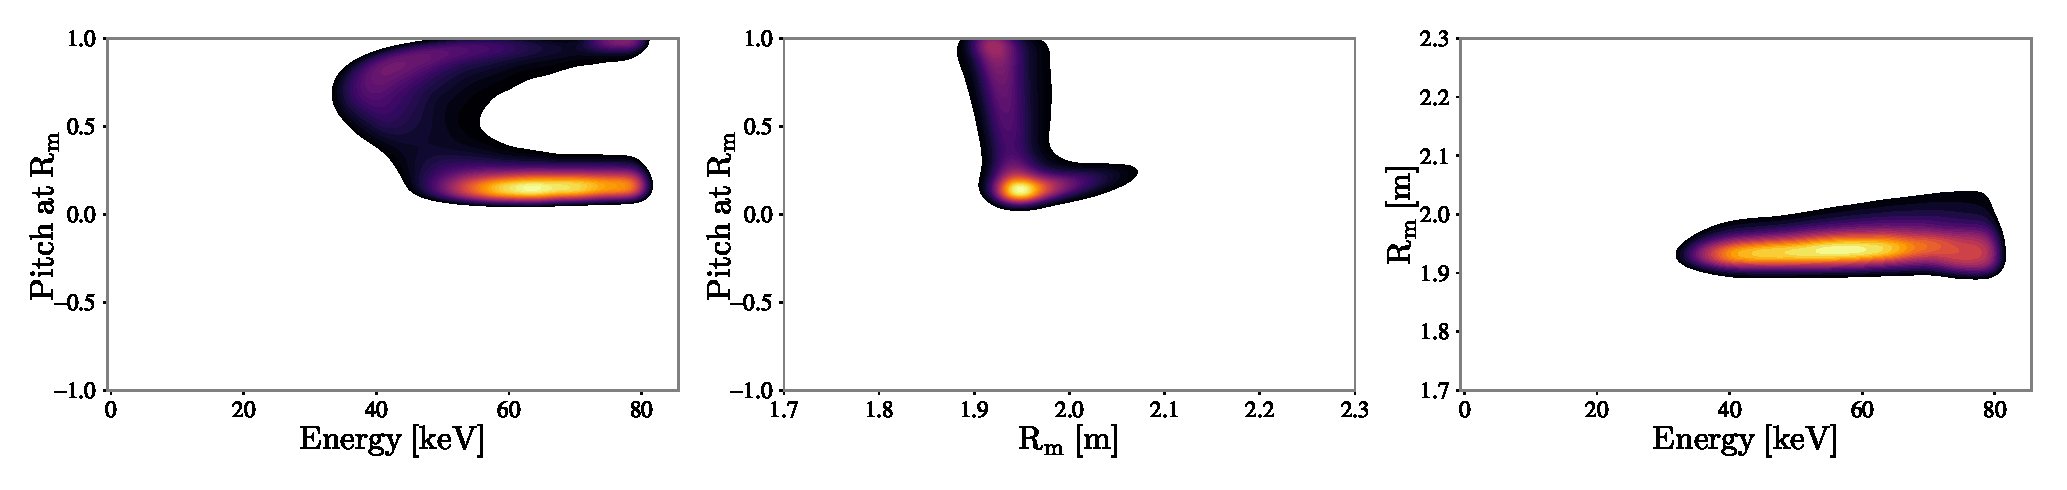
\includegraphics[width=15cm]{figures/fida_orbit_weight_blue_14.eps}
    \caption{Projections of the blue shifted ($\lambda = 652 \pm 0.2$ nm) FIDA orbit weight function for an oblique viewing chord with midplane intersection at R=1.9 m.}
    \label{fig:fida_blue}
\end{figure}
Unlike the red shifted orbit weight function, the blue shifted weight function is not sensitive to counter-passing particles; only showing sensitivity to orbits that are co-passing in the viewing region.

Like the other diagnostics, the spectra calculated using orbit weight functions closely matches the spectra produced by FIDASIM (Fig. \ref{fig:fida_orbit_spectra}). Also compared in the figure is the spectra calculated using velocity-space weight functions, which performs poorly in this case.
\begin{figure}[h!]
    \centering
    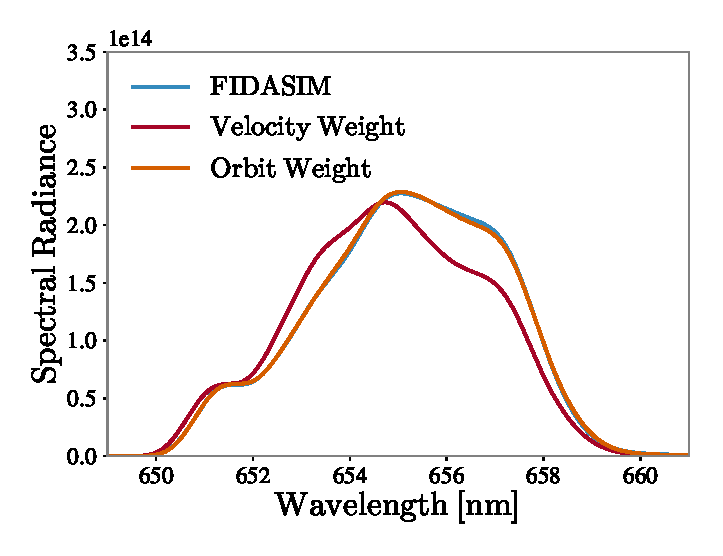
\includegraphics[width=10cm]{figures/fida_orbit_spectra.eps}
    \caption{FIDA Spectra for shot \#159243 @ 790 ms calculated by FIDASIM and by the FIDA orbit weight functions and Equation \ref{eq:orbit_tomography} for an oblique (Fig. \ref{fig:geometry}) viewing chord at $R = 2.1$ m.}
    \label{fig:fida_orbit_spectra}
\end{figure}




\chapter{Velocity-space Tomography}\label{chap:velocity-space_tomography}

The previous chapter discussed the theoretical underpinnings of diagnostic weight functions. In this and the next chapter we discuss their main application, the inference of the fast-ion distribution function from experimental measurements. As an appetizer for the main course of this thesis, Orbit Tomography, we will first discuss its precursor Velocity-space Tomography.

\section{Mathematical Formulation}
Velocity-space tomography, as the name suggests, uses velocity-space weight functions to infer a local approximation of the fast-ion distribution function---the distribution is local and approximate because, as we showed in the previous chapter, the weight functions are local and approximate.
Equation \ref{eq:vs_WF} can be discretized to form
\begin{equation} \label{eq:wf_discrete_single}
    s = \mathbf{w}^T \cdot \mathbf{f}\,,
\end{equation}
where $s$ is a scalar representing the measured signal, and the vectorized form of the velocity-space weight function and the local fast-ion distribution is given by $\mathbf{w}$ and $\mathbf{f}$ respectively. Equation \ref{eq:wf_discrete_single} alone is insufficient to infer a meaningful distribution function.
Since one pixel distributions are of limited use, multiple measurements and their corresponding weight functions are combined to create a system of linear equations:
\begin{equation}\label{eq:wf_discrete}
    \mathbf{s} = \mathbf{W}\cdot\mathbf{f}
\end{equation}
where $\mathbf{s}$ is a column vector of the measurements and $\mathbf{W}$ is a weight matrix where each $i^{th}$ row contains the weight function, $\mathbf{w}_i^T$, for the $i^{th}$ measurement, $s_i$. 
The number of elements of $\mathbf{f}$, which are colloquially called ``pixels'', are chosen to to be less than the number of measurements available in order to create an over-determined system of equations. 
Ideally, the value of $\mathbf{f}$ is found by solving the over-determined system of equations, however, this is not the case. Measurement noise and model inaccuracies prevent a direct application of linear algebra, requiring different methods to invert Equation \ref{eq:wf_discrete}. It is fortunate then that the tomographic techniques that have been used in plasma physics research in the past, provide a rich library of inversion methods to try.\cite{nagayama1981soft,koslover1986measurement,mcwilliams1987laboratory,reinhold1990excitation,Anton1996,zimmerman2005two,svensson2008current,odstrcil2012modern}

Forms of tomographic reconstructions has been used in plasma physics research for a number of decades, however,
despite the long history, a single best method has not emerged. This is because every tomography application is different. An inversion method well suited for one application may not be suitable for a different application. This is particularly true for Velocity-space Tomography since, unlike other types of tomography that use many measurements that are averaged over a line-of-sight, we use relatively few measurements that are averaged over a 2D area or, in the case of Orbit Tomography, a 3D volume. This precludes certain types of inversion methods such as Radon transforms. It also makes tomography much more difficult, since the many line-of-sight measurements of traditional tomography provide excellent discriminating information, which shrinks the possible set solutions significantly; the same cannot be said of the 2D/3D ``lines-of-sight'' of fast-ion tomography.

In order to determine their suitability for Velocity-space Tomography, in the following sections we will explore five different inversion methods that have been used in other applications and benchmark them against known theoretical distribution functions. We will then use the different methods to study the redistribution of fast-ions by a sawtooth crash. 

\section{Inversion methods}\label{sec:methods}
Measurement noise, error incurred by discretizing velocity-space, and the inherent flaws of velocity-space weight functions discussed in the previous chapter prevent an exact solution to Equation \ref{eq:wf_discrete}. We can instead use a probabilistic approach. Let's assume that the measured data, $\mathbf{s}$, is distributed according to a multivariate normal distribution,
\begin{equation}\label{eq:likelihood}
    \rm{prob}(\mathbf{s}|\mathbf{f},\mathbf{\Sigma}) \propto \exp{\left(-\frac{1}{2} (\mathbf{W}\cdot\mathbf{f} - \mathbf{s})^T \cdot \mathbf{\Sigma}^{-1} \cdot (\mathbf{W}\cdot\mathbf{f} - \mathbf{s})\right)}\,,
\end{equation}
where $\mathbf{\Sigma}$ is a diagonal matrix containing the variance/noise of the measured data. This probability is also known as the likelihood. We would like to find the value of $\mathbf{f}$ that maximizes the probability of observing the data. This can be reformulated as a minimization of the log-probability, which is equivalent to the classic least-squares minimization:
\begin{equation}\label{eq:least_squares}
    \mathrm{minimize} \left \lbrace \frac{1}{2}\left|\left| \mathbf{\overline{W}}\cdot\mathbf{f} - \mathbf{\overline{s}}\right|\right|^2 \right \rbrace 
\end{equation}
where the barred variables are normalized quantities: $\mathbf{\overline{W}} = \sqrt{\mathbf{\Sigma}^{-1}}\cdot\mathbf{W}$ and $\mathbf{\overline{s}}=\sqrt{\mathbf{\Sigma}^{-1}}\cdot\mathbf{s}$.
The minimum, $\mathbf{\hat{f}}$, of the above equation can be found analytically and is given by
\begin{equation}\label{eq:least_squares_solution}
    \mathbf{\hat{f}} = \left(\mathbf{\overline{W}}^T\cdot\mathbf{\overline{W}}\right)^{-1}\cdot\mathbf{\overline{W}}^T \cdot \mathbf{\overline{s}}
\end{equation}
This is known as the least-squares solution or the maximum likelihood solution.

The least-squares method is usually the first inversion technique tried and the first one discarded. While the overall idea behind the method is sound, least-squares solutions tend to fit the noise rather than the true underlying signal. This produces noisy and nonphysical solutions, limiting the least-squares method to situations where the experimental noise is very low and the model is very accurate, neither of which is the case for Velocity-space Tomography.
All is not lost, however, as there are numerous methods that can improve the least-squares solution.   

\subsection{Truncated Singular Value Decomposition} \label{sec:tsvd}
Truncated singular value decomposition (TSVD) is one method to reduce the effects of noise.
Rewinding some, the least-squares solution (Eq. \ref{eq:least_squares_solution}) can be written down as 
\begin{equation}
    \mathbf{\hat{f}} = \mathbf{\overline{W}}^+ \cdot \mathbf{\overline{s}}
\end{equation}
where
\begin{equation}\label{eq:pseudoinverse}
    \mathbf{\overline{W}}^+ = \left(\mathbf{\overline{W}}^T\cdot\mathbf{\overline{W}}\right)^{-1}\cdot\mathbf{\overline{W}}^T\,.
\end{equation}
This expression is known as the Moore-Penrose pseudoinverse. The pseudoinverse can also be constructed via the following expression,
\begin{equation}\label{eq:svd_pseudoinverse}
    \mathbf{\overline{W}}^+ = \mathbf{V} \cdot \mathbf{\Sigma}^+ \cdot \mathbf{U}^T \, ,
\end{equation}
where the $\mathbf{V}$, $\mathbf{\Sigma}$, and $\mathbf{U}$ matrices are calculated from the normalized weight matrix via its singular value decomposition (SVD),
\begin{equation} \label{eq:svd}
    \mathbf{\overline{W}} = \mathbf{U} \cdot \mathbf{\Sigma} \cdot \mathbf{V}^T \,,
\end{equation}
where $\mathbf{U}$ and $\mathbf{V}$ are unitary matrices, and $\mathbf{\Sigma}$ is a diagonal rectangular matrix containing, in decreasing order, the square roots of the non-zero eigenvalues of $WW^T$ and $W^T W$ \cite{Strang}. $\mathbf{\Sigma}^+$ is the pseudoinverse of $\mathbf{\Sigma}$, which is formed by replacing every non-zero diagonal element with its reciprocal.
Equations \ref{eq:svd_pseudoinverse} and \ref{eq:svd} can also be written as sums
\begin{equation}
\begin{split}
    \mathbf{\overline{W}} &= \sum_{j=1}^r \sigma_j\, \mathbf{u}_j \cdot \mathbf{v}_j^T  \\
    \mathbf{\overline{W}}^+ &= \sum_{j=1}^r \frac{\mathbf{v}_j \cdot \mathbf{u}_j^T}{\sigma_j}
\end{split}
\end{equation}
where $r$ is the number of non-zero singular values, $\mathbf{u}_j$ and $\mathbf{v}_j$ are the j$^{th}$ columns of $\mathbf{U}$ and $\mathbf{V}$, respectively, and $\sigma_j$ is the j$^{th}$ singular value.

While this is a bit of interesting mathematics, it is not immediately clear how this can improve the least-squares solution. Consider the following. Let the measured signal be composed of the true signal plus some noise: $\mathbf{s} = \mathbf{s}_{\rm{true}} + \boldsymbol{\epsilon}$. We can then express the least-square solution as the sum
\begin{equation}\label{eq:f_svd_sum}
    \mathbf{\hat{f}} = \sum_{j=1}^r \frac{\left(\mathbf{u}_j^T \cdot (\mathbf{s}_{\rm{true}} + \boldsymbol{\epsilon}) \right)}{\sigma_j} \mathbf{v}_j = \overbrace{\sum_{j=1}^r \frac{\left(\mathbf{u}_j^T \cdot \mathbf{s}_{\rm{true}} \right)}{\sigma_j} \mathbf{v}_j}^{\mathbf{f}_{\rm{true}}} + \overbrace{\sum_{j=1}^r \frac{\left(\mathbf{u}_j^T \cdot \boldsymbol{\epsilon} \right)}{\sigma_j} \mathbf{v}_j}^{\mathbf{f}_{\rm{noise}}}
\end{equation}
where the first sum is the true solution, $\mathbf{f}_{\rm{true}}$, and the last sum describes the effect of the noise, $\mathbf{f}_{\rm{noise}}$. For very small singular values, the least-squares solution can be completely dominated by the noise term. We can reduce the effect of the noise by truncating the sum after $k$ terms, eliminating the effects of the smallest singular values. However, since the measured signal cannot be separated from the noise, the truncation would also affect the first sum, making it impossible to reconstruct $\mathbf{f}_{\rm{true}}$ perfectly. In some situations, this is an acceptable trade-off. 

\subsection{Regularized Least-Squares}
Regularization is the process of adding additional information in order to solve an ill-posed inverse problem. Regularized least-squares is a family of methods that uses the ``regularize'' least-squares solution by adding a function to Equation \ref{eq:least_squares} that constrains the possible set of solutions to have certain properties defined by the regularizer. The regularized least-squares solution is then found by minimizing the modified least-squares problem
\begin{equation}\label{eq:regularized_least_squares}
    \mathrm{minimize} \left \lbrace \chi^2(\mathbf{x}) + \alpha \mathcal{R}(\mathbf{x}) \right \rbrace 
\end{equation}
where $\chi^2(\mathbf{x})$ is the original least-squares functional given in Equation \ref{eq:least_squares}, $\mathcal{R}(\mathbf{x})$ is the regularizing functional, and $\alpha$ is a hyper-parameter that controls the strength of the regularizer. From a probabilistic standpoint a regularizer is equivalent to a prior probability. 

In the following sections, we will explore 4 different regularizers: 0$^{th}$ and 1$^{st}$ order Tikhonov regularization, minimum Fisher information regularization, and maximum entropy regularization.

\subsubsection{0$^{th}$ and 1$^{st}$ Order Tikhonov Regularization}
Tikhonov regularization is the most commonly used form of regularization. The regularizer takes the form
\begin{equation}
    \mathcal{R}(\mathbf{x}) = ||\mathbf{L}\cdot\mathbf{x}||^2 \,,
\end{equation}
where $\mathbf{L}$ is called the Tikhonov matrix. This is a popular method because the minimum of the functional (Eq. \ref{eq:regularized_least_squares}) has an analytic solution given by
\begin{equation}\label{eq:tikhonov_solution}
    \mathbf{\hat{f}}_T = \left(\mathbf{\overline{W}}^T \cdot \mathbf{\overline{W}} + \alpha \mathbf{L}^T\cdot \mathbf{L} \right)^{-1} \cdot \mathbf{\overline{W}}^T \cdot \mathbf{s} \, . 
\end{equation}

The Tikhonov matrix determines the nature of the regularization. 
For instance, the simplest choice is to set $\mathbf{L}$ to be equal to the identity matrix i.e. 0$^{th}$ order Tikhonov regularization. When the functional(Eq. \ref{eq:regularized_least_squares}) is minimized with this regularizer, large absolute values in $\mathbf{f}$ are penalized, which encourages a solution with a smaller variance.

Another popular choice is to use a finite-difference operator as a Tikhonov matrix i.e. 1$^{st}$ order Tikhonov regularization. This regularizer penalizes large gradients, which promotes smooth solutions.
To use this regularizer the $\mathbf{L}^T \mathbf{L}$ term in Equation \ref{eq:tikhonov_solution} becomes
\begin{equation}
    \mathbf{L}^T \cdot \mathbf{L} = 2mE \, \boldsymbol{\nabla}_E^T \cdot \boldsymbol{\nabla}_E + \frac{m}{2E}\left(1-p^2 \right) \, \boldsymbol{\nabla}_p^T \cdot \boldsymbol{\nabla}_p \, .
\end{equation}
where $\boldsymbol{\nabla}_{E}$ and $\boldsymbol{\nabla}_{p}$ are matrix representations of finite difference operators in energy and pitch space respectively\cite{jacobsen_stagner2016}.

\subsubsection{Minimum Fisher Information Regularization}
Minimum Fisher information regularization uses a regularizer of the form\cite{Anton1996}
\begin{equation}
    \mathcal{R}(g(x)) = \int \frac{g'(x)^2}{g(x)} dx\,.
\end{equation}
The minimum Fisher information regularizer penalizes large gradients normalized by the function values.
The normalization ensures the smoothing effect is strongest where the function is smallest. This should, in principle, allow for solutions that have both sharp peaks and smooth features.

Typically, using a regularizer of this form would require the use of a non-linear optimization algorithm to minimize the functional. However, in a previous application of this method\cite{Anton1996}, an iterative algorithm that formulates the minimum Fisher regularizer as a Tikhonov matrix was developed.  
The algorithm is as follows.

The first solution, $\mathbf{f}^{(1)}$, is found using 1$^{st}$ order Tikhonov regularization.
For each subsequent iteration, the $\mathbf{L}^T \cdot \mathbf{L}$ term in Equation \ref{eq:tikhonov_solution} is set to
\begin{equation}
    \mathbf{L}^T \mathbf{L} = 2mE \boldsymbol{\nabla}_E^T \cdot \mathbf{M}^{(n)} \cdot \boldsymbol{\nabla}_E + \frac{m}{2E} \left(1-p^2 \right) \boldsymbol{\nabla}_p^T \cdot \mathbf{M}^{(n)}\cdot\boldsymbol{\nabla}_p \, ,
\end{equation}
where the elements of the matrix, $\mathbf{M}$ are given by
\begin{equation}
\begin{split}
    M^{(n)}_{i,j} &= \frac{1}{f_i^{(n-1)}} \, \delta_{i,j} \qquad \mathrm{if} \qquad f^{(n-1)}_i > 0\\
    M^{(n)}_{i,j} &= M^{(n)}_{max} \, \delta_{i,j} \qquad\; \mathrm{if} \qquad f^{(n-1)}_i \leq 0 \, ,
\end{split}
\end{equation}
where $M^{(n)}_{max}$ is the largest $M^{(n)}$ for $f^{(n-1)}_i > 0$.
The solution converges after a few iterations ($n\sim3$).

\subsubsection{Maximum Entropy Regularization}
The last inversion method is maximum entropy regularization, which seeks to find the solution that maximizes entropy. This is done by using a regularizer of the form 
\begin{equation}
	\mathcal{R}(\mathbf{x}) = -\sum_{i=1}^N (x_i-m_i-x_i\ln(x_i/m_i)) \, ,
\end{equation}
which is the negative of the Shannon information entropy. 
The regularizer is minimized when $x_i = m_i$. Thus $m_i$ is called the default model as it is the value $x_i$ will take in the absence of data. Thus, the maximum entropy regularizer promotes solutions that are ``close'' to the default model, only deviating from it in order to better fit the data. In this work, the default model is set to be constant in order to prevent biasing of the solution, however, the default model could be chosen to be given by a theoretical model, which is advantageous in certain situations. 
The minimum of the functional, called the maximum entropy solution, is found using a general non-linear optimization library \cite{giffin2007updating,wachter2006ipopt,LubinDunningIJOC}.

\subsection{Hyper-parameter Optimization}
All of the discussed inversion methods rely on hyper-parameters that need to be chosen \textit{a priori}: the number of singular values, $k$, for truncated SVD and the regularizer strength parameter, $\alpha$, for regularized  least-squares. Usually, the hyper-parameters are chosen to give the best looking results. We instead us the L-curve method\cite{Hansen2007} to choose hyper-parameters systematically. 
In the L-curve method, reconstructions are calculated for a range of hyper-parameter values, storing both the regularizer, $\mathcal{R}(\mathbf{x})$, and the goodness-of-fit, $\chi^2(\mathbf{x})$, values. When plotted on a loglog plot, the regularizer and the goodness-of-fit form a L shape (Fig. \ref{fig:L_curve}). The right part shows the associated curvature. The point with maximum curvature is the corner point. The hyper-parameter value at the corner of the L-curve is chosen because it represents a balance between fitting the data and regularizing the solution. The corner is found by finding the point of maximum curvature of the L-curve.
\begin{figure}[h!]
    \centering
    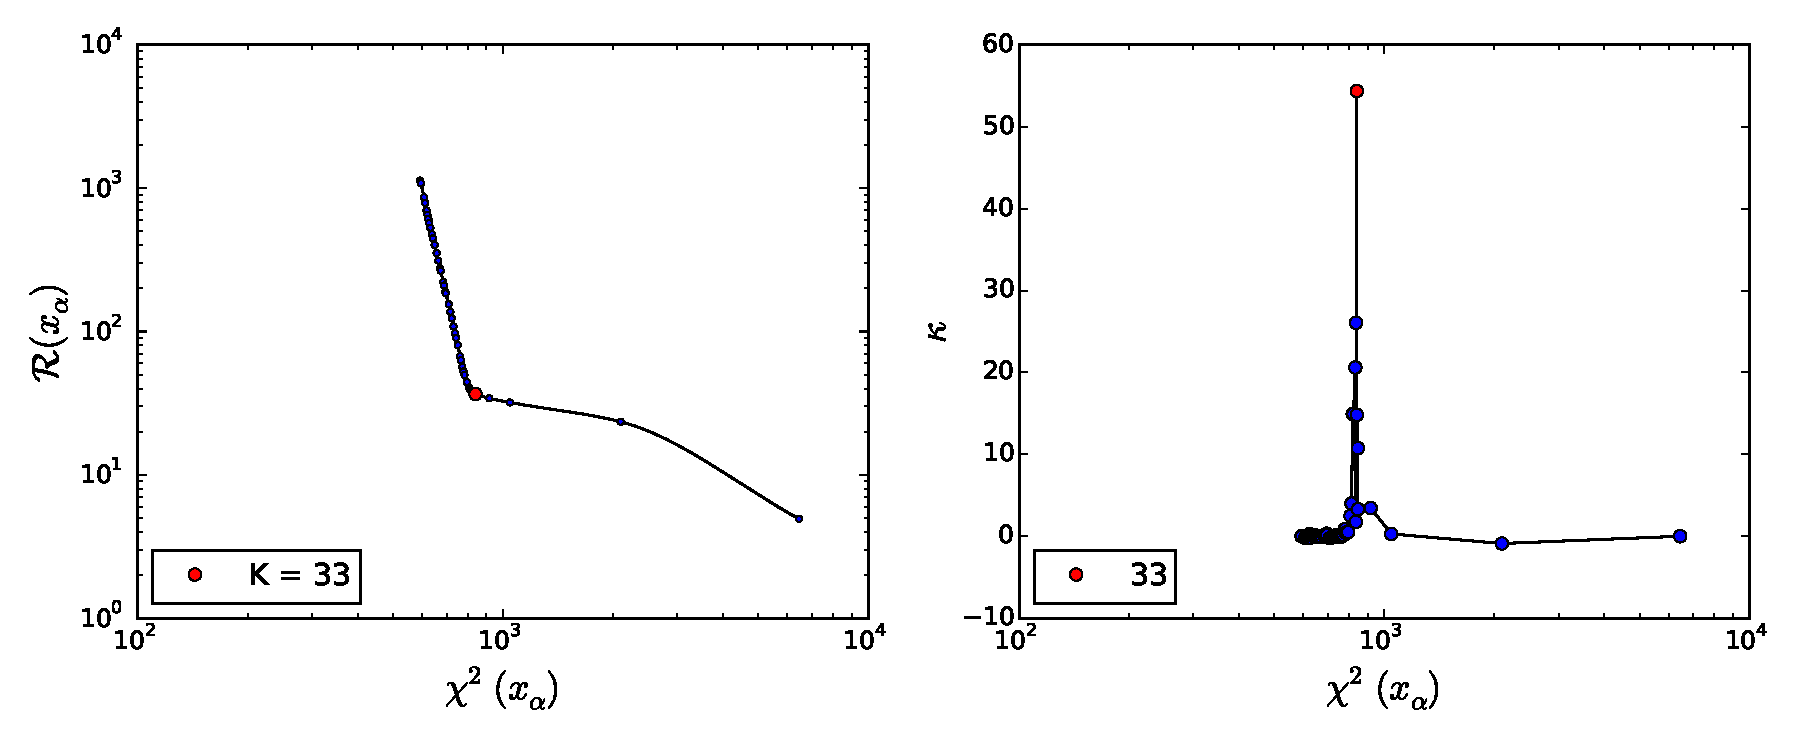
\includegraphics[width=0.95\textwidth]{inversion_methods/figure3.eps}
    \caption{Example of how to chose the hyper-parameter based on the L-curve method for the truncated SVD inversion method. The norm of the solution is used as a proxy for the regularizer. Left: loglog plot of the L-curve. Right: Curvature of the L-curve. The point of highest curvature/corner is indicated by the red point.}
    \label{fig:L_curve}
\end{figure}

\section{Benchmarks using Synthetic Data}\label{sec:results_synth}
In this section, we compare the different inversion methods using synthetic data calculated using Equation \ref{eq:wf_discrete} and known distribution functions. This enables us to compare the performance of the inversion methods using quantitative metrics since the true solutions are known.

\subsection{Benchmarking Apparatus}\label{sec:AUG_fida}
\subsubsection{Diagnostic Setup}
The benchmarking exclusively uses synthetic FIDA measurements. We base the diagnostic geometry on the FIDA systems installed at ASDEX Upgrade, which consists of five radial arrays each intersecting the Q3 neutral beam. From each system, a line of sight that views the center of the plasma is chosen (Fig. \ref{fig:FIDA_geometry}). 
\begin{figure}[ht]
    \centering
    \includegraphics[width=15cm]{inversion_methods/figure2.eps}
    \caption{Sketch of the geometry of the FIDA diagnostic set-up. a) Top view of the ASDEX Upgrade tokamak showing the NBI beam in grey and the FIDA lines-of-sight in colours. Only the lines-of-sight used here are shown. b) Poloidal cross-section showing that the FIDA measurement volume used here is slightly on the low-field side of the ASDEX Upgrade tokamak.} \label{fig:FIDA_geometry}
\end{figure}
The lines-of-sight originate from different positions in the plasma wall and intersect the neutral beam at approximately the same position---a requirement for Velocity-space Tomography.
Each view has a different angle between its line of sight and the magnetic field, probing different regions of the velocity space\cite{Salewski2014a}. In the plasma center, the respective angles are 14$^\circ$, 73$^\circ$, 103$^\circ$, 133$^\circ$ and 153$^\circ$.
Descriptions of ASDEX Upgrade's FIDA systems are found in Reference \cite{Weiland2015}.

\subsubsection{Test Distributions}
Three different velocity distributions are investigated: a Gaussian distribution, a bi-Maxwellian distribution, and a  NBI-distribution simulated by TRANSP/NUBEAM\cite{Pankin2004}. The three distributions are shown in Figure \ref{fig:original_distributions}. These three distribution functions pose different challenges to the inversion methods.
The Gaussian distribution represents a localized source of fast ions, a proxy for the peaks at the injection energies found in the distributions of neutral beam heated discharges. 
The bi-Maxwellian is a wide function covering the entire pitch range. Here the challenge is to recreate the large-scale structure. Lastly, we study a neutral beam injection distribution function. This is an important test case as it should be very similar to the distribution functions in experiments with NBI heating. The challenge here is the structural complexity on both small and large scales. 
\begin{figure}[h!]
    \centering
    \subfigure[Gaussian.\label{fig:orig_blob}]{%
    	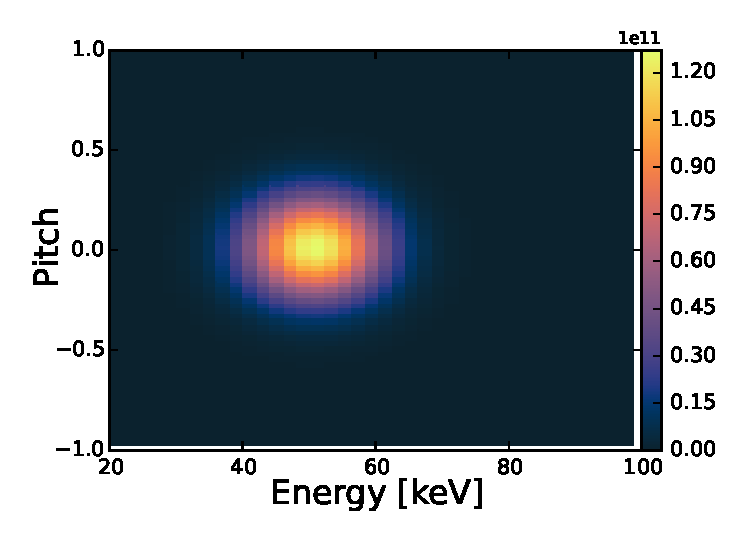
\includegraphics[width=0.30\textwidth]
    	{inversion_methods/figure4a.eps}
    }
    \subfigure[Bi-Maxwellian.\label{fig:orig_bimax}]{%
    	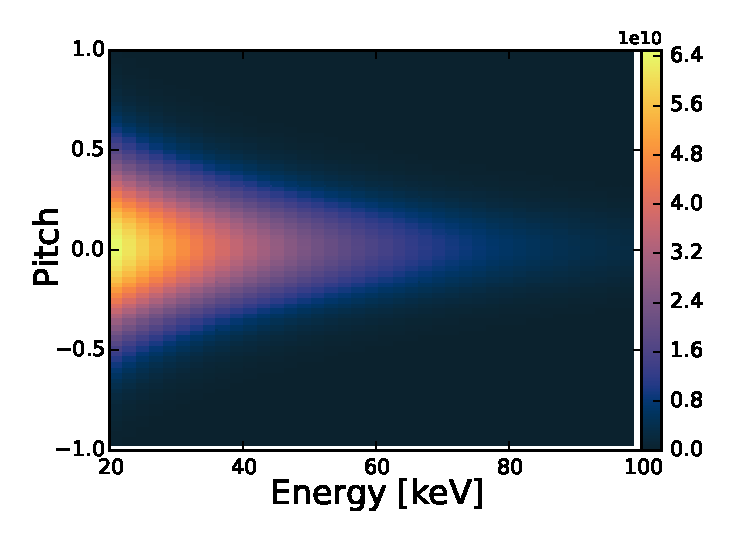
\includegraphics[width=0.30\textwidth] 
    	{inversion_methods/figure4b.eps}
    }
    \subfigure[NBI.\label{fig:orig_transp}]{%
    	\includegraphics[width=0.30\textwidth] 
    	{inversion_methods/figure4c.eps}
    }
    \caption{Test velocity distributions functions as a function of energy and pitch. The functions are given in units of [ions/keV/cm$^3$]} \label{fig:original_distributions}
\end{figure}

\subsubsection{Simulating Measurement Noise}\label{sec:uncertainty}
A realistic model of spectra noise is used in the benchmarking. The photon noise of FIDA light scales approximately with the square root of the signal. However, in the absence of FIDA light the photon noise is dominated by the amount of bremsstrahlung, $B$, setting a lower limit on the noise level. 
These two effects are modelled as
\begin{equation}\label{eq:S_noisy}
    S_{\rm{noisy}} = S_{\rm{true}} + k \left\langle \sqrt{S_{\rm{true}}} \right\rangle \eta \quad \eta \sim \mathcal{N}(0,\max\left(\sqrt{B},\sqrt{S_{\rm{true}}}\right)) ,
\end{equation}
where $S_{\rm{noisy}}$ is the noisy spectrum, $S_{\rm{true}}$ is the true noise-free spectrum, $\left\langle \right\rangle$ denotes a mean, and $k$ is a scaling constant that allows us to vary the noise level.
By varying the noise level we can investigate how robust the methods are against noise. Figure \ref{fig:spectra_transp} shows examples of the standard deviation of the synthetic spectra calculated using the NBI test distribution for $k=0.1$, $k=0.5$ and $k=0.9$. 
The noise level of actual FIDA measurements depends on the plasma parameters, but a $k$ value in the range 0.3-0.5 represents the typical noise level in a discharge.
\begin{figure}[h!]
    \centering
    \includegraphics[width=0.70\textwidth]
    {inversion_methods/figure5.eps}
    \caption{Examples of the average noise levels in the synthetic spectra calculated using the NBI test distribution and equation (\ref{eq:S_noisy}) for k=\{0.1, 0.5 and 0.9\}. The width of the spectra corresponds to the standard deviation of the noise for the given $k$-value.}
    \label{fig:spectra_transp}
\end{figure}

\subsection{Quantitative Comparison Metrics}
The noise in the synthetic spectra propagates through the inversion process. If a single synthetic spectra is used, one of the inversion methods could get lucky and perform better then the rest.
In order to quantify the \textit{average} performance of the inversion methods, the results of the inversion methods are averaged over an ensemble of 25 noisy spectra. The variance of the reconstructions is used to quantify the effects of noise.

The inversion method itself also introduces a type of error. For instance, an inversion method may systematically bias solutions to be overly smooth. We can quantify this bias by finding the difference between the mean distribution for a given $k$ and the true distribution:
\begin{equation}\label{eq:bias}
    \mathrm{bias} = \mathbf{\hat{f}}_\mu - \mathbf{f}_{\rm{true}} \, , 
\end{equation}
where $\mathbf{\hat{f}}_\mu$ is the mean distribution and $\mathbf{f}_{\rm{true}}$ is the true distribution. 
Combining the bias with the variance, we define a measure of the total uncertainty of a pixel by the mean squared error, MSE, given by
\begin{equation}\label{eq:MSE}
    \mathrm{MSE} = \mathrm{variance} + \mathrm{bias}^2 \, .
\end{equation}

The MSE summed over the inversion along with the ratio of the inferred to the true fast-ion density are used as quantitative performance metrics.

\subsection{Inversion Results}
\subsubsection{Gaussian Distribution}
Figure \ref{fig:tomos_blob} shows reconstructions of the Gaussian distribution calculated with the different inversion methods for various noise levels. 
All methods reconstruct the position of the Gaussian distribution well. The characteristic widths of the Gaussians are approximately right but tend to be slightly larger than in the original test distribution. Measurement noise enhances this trend. We further observe the appearance of jitter in the reconstructions throughout velocity space. 
The minimum Fisher information and maximum entropy regularization methods stand out from the other methods in that they resemble the original function the most and exhibit the least jitter. This suggests superior resolution performance of these methods. Table \ref{tab:synthetic_parameters_blob} contains the true center coordinates and width of the Gaussian distribution in both energy and pitch. Furthermore, it contains the values obtained from the $k=0.5$ reconstructions calculated using the five different methods. All methods find the center coordinates well. The minimum Fisher information and maximum entropy methods produce significantly more peaked distributions which is seen in their ability to better match the true width of the Gaussian. 
\begin{table}[h!]
    \caption{\label{tab:synthetic_parameters_blob} Parameters of the Gaussian test distribution. Parameters are found by fitting the reconstructed distributions to the analytic form of the true distribution.}
    \begin{tabular}{@{}r|llllll}
     & \textbf{True} & \textbf{SVD} & \textbf{T0} & \textbf{T1} & \textbf{MFI} & \textbf{ME} \\
    \hline\hline
    $\mu_E$ [keV] & 50 & 49.37$\pm$0.22 & 49.55$\pm$0.19 & 48.57$\pm$0.21 &  48.45$\pm$0.06 & 50.78$\pm$0.07 \\
    $\sigma_E$ [keV] & 10 & 15.16$\pm$0.32 & 15.34$\pm$0.27 & 16.61$\pm$0.30 & 11.24$\pm$0.08 & 8.87$\pm$0.10 \\
    $\mu_p$ [-] & 0 & 0.008$\pm$0.005 & -0.001$\pm$0.004 & -0.001$\pm$0.004 & -0.011$\pm$0.001 & 0.035$\pm$0.002 \\
    $\sigma_p$ [-] & 0.25 & 0.325$\pm$0.007 & 0.329$\pm$0.006 & 0.317$\pm$0.006 & 0.228$\pm$0.02 & 0.242$\pm$0.003 \\
    \hline
    \end{tabular}
\end{table}

\begin{figure}[h!]
    \centering
    \includegraphics[width=0.95\textwidth]{inversion_methods/figure6.eps}
    \caption{Reconstructions of the Gaussian distribution (Fig. \ref{fig:orig_blob}) from on synthetic measurements using various inversion methods and noise levels. The noise level $k$ is defined in equation (\ref{eq:S_noisy}). Distributions have units of [ions/keV/cm$^3$] } 
    \label{fig:tomos_blob}
\end{figure}

\subsubsection{Bi-Maxwellian Distribution}
Figure \ref{fig:tomos_bimax} shows the reconstructions of the bi-Maxwellian distribution function. The large-scale shape of the distribution is reproduced by all five inversion methods. The pitch angle symmetry and long tail at $p=0$ is also reproduced.
The first-order Tikhonov, minimum Fisher information, and maximum entropy methods reproduce the distribution particularly well. Table \ref{tab:synthetic_parameters_bimax} contains the true parallel and perpendicular temperatures used in calculating the bi-Maxwellian and the values obtained from fitting the $k=0.5$ reconstructions to the analytic form of the bi-Maxwellian. For the bi-Maxwellian distribution, the minimum Fisher information method most closely recreates the true values.
\begin{table}[h!]
    \caption{\label{tab:synthetic_parameters_bimax} Parameters of the bi-Maxwellian test distribution. Parameters are found by fitting the reconstructed distributions to the analytic form of the true distribution.}
    \begin{tabular}{@{}r|llllll}
     & \textbf{True} & \textbf{SVD} & \textbf{T0} & \textbf{T1} & \textbf{MFI} & \textbf{ME} \\
    \hline\hline
    $E_\parallel$ [keV] & 3 & 5.12$\pm$0.19 & 5.34$\pm$0.18 & 4.98$\pm$0.09 & 2.94$\pm$0.06 & 4.09$\pm$0.13 \\
    $E_\perp$ [keV] & 20 & 24.36$\pm$0.73 & 26.26$\pm$0.73 & 23.79$\pm$0.35 & 22.51$\pm$0.32 & 24.73$\pm$0.61 \\
    \hline
    \end{tabular}
\end{table}
\begin{figure}[h!]
    \centering
    \includegraphics[width=0.95\textwidth]{inversion_methods/figure7.eps}
    \caption{Reconstructions of the bi-Maxwellian (Fig. \ref{fig:orig_bimax}) distribution from synthetic measurements using various inversion methods and noise levels. The noise level $k$ is defined in equation (\ref{eq:S_noisy}). Distributions have units of [ions/keV/cm$^3$] }
    \label{fig:tomos_bimax}
\end{figure}

\subsubsection{NBI Distribution}
Figure \ref{fig:tomos_transp} shows reconstructions of the NBI distribution function for various noise levels and inversion methods.
This fast-ion distribution function is typical for neutral beam injection with two co-current beams with injection energies at 80 keV and 70 keV and one counter-current beam with an injection energy of 70 keV. 
Therefore, this distribution function is a more difficult test case. 
The overall shape of the NBI distribution function is reproduced by all five inversion methods. The protrusion at pitches of about 0.7 originates from the co-current beam injection, and the weaker protrusion at pitches of -0.7 originate from the counter-current beam injection. All reconstructions show the full energy beam injection peak for co-current injection (positive pitch) at larger energies than that for counter-current injection (negative pitch). 
The first-order Tikhonov, minimum Fisher information and maximum entropy regularization results in smooth reconstructions. This makes the overall shape of the function with protrusions at positive and negative pitches stand out most clearly. 
The local maxima due to the beam injection peaks at full, half and third energies are recreated by the maximum entropy method in the case of low noise ($k=0.1$). They are also visible in the SVD and zeroth-order Tikhonov tomographies at low noise, however the peaks are accompanied by other artifacts.
For larger noise levels, none of the methods are able to resolve more than one peak.
\begin{figure}[h!]
    \centering
    \includegraphics[width=0.95\textwidth]{inversion_methods/figure8.eps}
    \caption{Tomographies of the beam distribution from figure \ref{fig:orig_transp} in units of [ions/keV/cm$^3$] based on synthetic measurements using various inversion methods and noise levels. The noise level $k$ is defined in equation (\ref{eq:S_noisy}).} \label{fig:tomos_transp}
\end{figure}

The uncertainties of the reconstructions of the NBI distribution are shown in Figure \ref{fig:uncertainties_transp} for a noise level of $k=0.5$.
The top row shows the square root of the variance of the reconstructions. 
Compared with the values of the reconstructions in Figure \ref{fig:tomos_transp}, the uncertainties are about one order of magnitude smaller, and smallest for first-order Tikhonov and minimum Fisher information regularization. 
The middle row shows the bias.
Negative values denote regions where too few ions are placed, positive values denote regions where too many ions are placed.
The beam peaks are seen in the bias, especially for first-order Tikhonov, minimum Fisher information and maximum entropy regularization as these are only able to resolve the peaks for low noise levels.
The last row shows the square root of the mean squared error. 
The main contribution to the uncertainty is the bias.
\begin{figure}[h!]
    \centering
    \includegraphics[width=0.95\textwidth]{inversion_methods/figure10.eps}
    \caption{Uncertainties for the reconstructions of the beam distribution in units of [ions/keV/cm$^3$]. All uncertainties are calculated for a noise level of $k=0.5$.}
    \label{fig:uncertainties_transp}
\end{figure}

\subsubsection{Noise Scaling}
Figure \ref{fig:Qfigs_tomos} shows the behaviour of the performance parameters as a function of noise level. Figures \ref{fig:Q1_blob}, \ref{fig:Q1_bimax} and \ref{fig:Q1_transp} show the total mean squared error.
The mean squared error increases for larger noise levels for all inversion methods and test distributions. 
The minimum Fisher information regularization method has the lowest mean squared error for all test distributions. 
Figures \ref{fig:Q2_blob}, \ref{fig:Q2_bimax} and \ref{fig:Q2_transp} show the density ratios. The general trend is that the methods produce a lower density ratio for large error levels. Thus, for very large noise levels the absolute values of an inferred density obtained from a reconstruction might be unreliable. For the Gaussian test distribution, the minimum Fisher information and maximum entropy methods are very good at recreating the correct density. The other three methods overestimate the amount of ions present. This is also the case for the bi-Maxwellian distribution but not to the same extent. 
For the NBI test distribution the spread in densities is smaller than for the other cases.
\begin{figure}
    \centering
    \subfigure[Total MSE, Gaussian\label{fig:Q1_blob}]{%
    	\includegraphics[width=0.45\textwidth]{inversion_methods/figure9a.eps}	
    }
    \subfigure[Density ratio, Gaussian\label{fig:Q2_blob}]{%
    	\includegraphics[width=0.45\textwidth]{inversion_methods/figure9b.eps}
    }
    \subfigure[Total MSE, bi-Maxwellian\label{fig:Q1_bimax}]{%
    	\includegraphics[width=0.45\textwidth]{inversion_methods/figure9c.eps}
    }
    \subfigure[Density ratio, bi-Maxwellian\label{fig:Q2_bimax}]{%
    	\includegraphics[width=0.45\textwidth]{inversion_methods/figure9d.eps}
    }
    \subfigure[Total MSE, NBI\label{fig:Q1_transp}]{%
    	\includegraphics[width=0.45\textwidth]{inversion_methods/figure9e.eps}
    }
    \subfigure[Density ratio, NBI\label{fig:Q2_transp}]{%
    	\includegraphics[width=0.45\textwidth]{inversion_methods/figure9f.eps}
    }
    \caption{Noise scaling of the reconstructions of the test distributions. The left column shows the total mean squared error. The right column shows the density ratio. }
    \label{fig:Qfigs_tomos}
\end{figure}

\section{Redistribution of Fast-ions by a Sawtooth Crash}\label{sec:results_real}
A sawtooth crash is a periodic plasma instability which can occur when the central safety factor drops below one. It changes the magnetic field topology and has been observed to redistribute particles and energy from the center of the plasma. Furthermore, it has been observed on several machines that passing fast ions are redistributed more strongly compared to trapped ions \cite{Nielsen2011,Muscatello2012,Geiger2015,weiland2016}.
Here we use the five different inversion methods to investigate the effect of a sawtooth on the central fast-ion population in ASDEX Upgrade. Figure \ref{fig:31557_timetraces} shows time traces from AUG discharge \#31557. The sawtooth crashes are evident in the central electron density as well as the central electron and ion temperatures. 
\begin{figure}[h!]
    \centering
    \includegraphics[width=0.75\textwidth]{inversion_methods/figure12.eps}
    \caption{Time traces of AUG discharge \#31557. a) Toroidal magnetic field, total injected NBI power and the plasma current. b) Ion and electron temperatures and electron density at $\rho_p=0.1$.} \label{fig:31557_timetraces}
\end{figure}
Experimental FIDA spectra from just before and after the sawtooth crash in ASDEX Upgrade discharge \#31557 at 2.25~s was used in this analysis. The same diagnostic setup used in the benchmarks is used here.
Figure \ref{fig:tomos_sawtooth} shows the reconstructed distributions from just before and after the crash and Figure \ref{fig:uncertainties_sawtooth} shows the uncertainties of the reconstructions of the pre-crash distribution.
\begin{figure}[h!]
    \centering
    \includegraphics[width=0.95\textwidth]
    {inversion_methods/figure13.eps}
    \caption{Reconstructed fast-ion distributions before and after a sawtooth crash calculated using the different inversion methods.} \label{fig:tomos_sawtooth}
\end{figure}
\begin{figure}[h!]
    \centering
    \includegraphics[width=0.95\textwidth]{inversion_methods/figure14.eps}
    \caption{Measures of uncertainties using the different regularization methods. The bias is calculated using the ``true'' distribution that is calculated using TRANSP's Kadomstev model.} \label{fig:uncertainties_sawtooth}
\end{figure}

The significant drop in fast ion density during the sawtooth crash is seen by all the inversion methods. By comparing the absolute values of the reconstructions with the uncertainties, we can identify the velocity-space regions where we can be confident in the result. 
Figure \ref{fig:tomos_sawtooth_normalized_with_MSE} shows the reconstructions normalized by $\sqrt{\mathrm{MSE}}$ for the five inversion methods. To calculate the bias after the sawtooth crash, the Kadomtsev model as implemented in TRANSP is used to model the effect of the sawtooth crash on the fast ions.
The parts of velocity space where the values are large correspond to regions where we are confident in the results and regions with low values correspond to uncertain regions. It is seen that the part of velocity space at the full energy peak at 60 keV is very uncertain for all inversion methods. This is because the methods are not able to resolve the peak given the choice of hyper-parameter. 
\begin{figure}[h!]
    \centering
    \includegraphics[width=0.95\textwidth]{inversion_methods/figure15.eps}
    \caption{Reconstructions of the ion velocity distribution normalized with $\sqrt{\mathrm{MSE}}$ before (top row) and after (bottom row) the sawtooth crash.}
    \label{fig:tomos_sawtooth_normalized_with_MSE}
\end{figure}
 
To further investigate the velocity-space dependence of the change in the fast-ion distribution function, we calculate the relative change:
\begin{equation}
\Delta \mathbf{\hat{f}}_{rel} = \frac{\mathbf{\hat{f}}_{after} - \mathbf{\hat{f}}_{before}}{\mathbf{\hat{f}}_{before}}  \, .
\end{equation}
The relative change is calculated for every regularization method and plotted in Figure \ref{fig:tomos_sawtooth_rel}. 
The top row shows the relative change as a function of energy and pitch. The bottom row shows the uncertainties of the relative change.
The variance of the relative change is calculated from an ensemble of relative changes, which was generated by sampling within the error bars of the experimental spectra.
\begin{figure}[h!]
    \centering
    \includegraphics[width=0.95\textwidth]{inversion_methods/figure16.eps}
    \caption{Relative change of the fast-ion velocity distribution function.} \label{fig:tomos_sawtooth_rel}
\end{figure}
The velocity-space dependence of the relative change is especially clear in the first-order Tikhonov and the minimum Fisher information figures as the amount of jitter in these reconstructions is significantly smaller compared to the other methods. 
Both first-order Tikhonov and minimum Fisher information suggest that ions with large pitch values are redistributed more compared to ions with pitch close to zero. 
This trend is also confirmed by the singular value decomposition, zeroth-order Tikhonov and maximum entropy in the regions where the reconstructions are reliable.
The unreliable regions are shown as those with large standard deviation compared with amplitudes of the reconstructions. 
Similar trends were observed previously using singular value decomposition \cite{Geiger2015} and a variant of a first-order Tikhonov \cite{Weiland2015}.
Figure \ref{fig:tomos_sawtooth_rel_1D} shows the ratio of the post-crash distribution to the pre-crash distribution integrated over energy as a function of pitch for all five inversion methods. Thus it is a measure of the pitch dependence of the change in the fast ion distribution function. 
For pitch values close to zero all inversion methods except maximum entropy predict a redistribution level of between 10\% and 20\%.
For pitch values above 0.4 the redistribution level increases to between 30\% and 40\% as seen by all five inversion methods. For negative pitch values, where very few ions are present, it isn't possible to determine the amount of redistribution.
\begin{figure}[h!]
    \centering
    \includegraphics[width=0.70\textwidth]{inversion_methods/figure17.eps}
    \caption{Ratio of the fast-ion velocity-space distribution functions before and after the crash integrated over energy shown as a function of pitch.} \label{fig:tomos_sawtooth_rel_1D}
\end{figure}

\section{Discussion}
In order to calculate the true bias of a given reconstruction, it is necessary to know the true distribution. This makes it impossible to calculate the true bias of a reconstruction from experimental measurements. Here, we have used a TRANSP distribution and the Kadomtsev model to generate an estimate of the true distribution. 
However, in other cases it might not be possible to calculate a good quantitative estimate. 
In these cases, the best one can do is estimate a qualitative bias based on the general behaviour of a inversion method.
On the other hand, uncertainties based solely on the propagation of measurement uncertainties through a given inversion method only represents the spread of obtainable solutions, and thus can be misleading since they can be made almost arbitrarily small, simply by over-regularizing.

It is seen that when the noise level is not too large, 
the first-order Tikhonov, minimum Fisher information and maximum entropy regularization methods can reconstruct the overall shape of the true distribution function very well.
However, the first-order Tikhonov and minimum Fisher information methods lack capability to resolve very fine and detailed features.
For large noise levels, the maximum entropy has a tendency to produce solutions with large variances.
Truncated SVD and zeroth-order Tikhonov can resolve fine details, especially for measurements with low noise levels. However, they often produce features in wrong parts of velocity space.

It is seen that the absolute values of a derived quantity such as the fast-ion density depend on the noise level in the data. However, we find that the ratio of such quantities is less sensitive to the specific noise level and bias. Hence, we can make statements about changes in such quantities with greater confidence than about the absolute values themselves since biases introduced by the inversion methods will tend to cancel. For example, the bias in the reconstructions tends to be similar before and after a sawtooth crash, and hence it partly cancels in the relative change.

\chapter{Orbit Tomography}\label{chap:orbit_tomography}

%Figure \ref{fig:orbit_fida_spectra}d shows how different spatial locations are weighted by the orbits.
In this chapter we develop Orbit Tomography, a method that uses orbit weight functions to infer the full fast-ion distribution function from experimental measurements.

Recall from Chapter \ref{chap:weights} that the forward model of a diagnostic can be linearized into the following form,
\begin{equation}\label{eq:S_linear}
    s = \sum_k n_k w(\mathbf{J}_k) \;,
\end{equation}
where $s$ is the diagnostic signal, $n_k$ is the number of fast ions on the k$^{th}$ orbit, and $w(\mathbf{J}_k)$ is the orbit's weight function.
In the infinite limit, Equation \ref{eq:S_linear} is an exact representation of the diagnostic's forward model. Truncating the number of orbits reduces the accuracy of the representation but allows for the forward model to be discretized,
\begin{equation}
    s = \mathbf{w}^T\cdot\mathbf{n}\,,
\end{equation}
where each element of $\mathbf{w}$ and $\mathbf{n}$ is the orbit weight function and number of fast-ions on the orbit, respectively. When multiple measurements are available, they can be combined to form a system of linear equations,
\begin{equation}\label{eq:Wxn}
    \mathbf{s} = \mathbf{W}\cdot\mathbf{n}\,,
\end{equation}
where each row of $\mathbf{W}$ contains the weight vector, $\mathbf{w}^T$, for each measurement. Similar to Velocity-space Tomography, the system of linear equations can be solved for the number of fast ions on each orbit, $\mathbf{n}$. Since orbit weight functions are used, instead of velocity-space weight functions, we call the process of solving the system Orbit Tomography.
In addition to the increased fidelity of the linearized forward model, Orbit Tomography has several other advantages over Velocity-space Tomography.

\begin{figure}[h!]
    \centering
    \includegraphics[width=15cm]{figures/orbit_fida_spectra.eps}
    \caption{FIDA orbit weights/spectra produced by three different orbits: trapped ($\rm{\mathbf{J}=(50\;keV,\;0.5,\;2.1\;m)}$), co-passing ($\rm{\mathbf{J}=(50\;keV,\;0.7,\;2.1\;m)}$), and counter passing ($\rm{\mathbf{J}=(50\;keV,\;-0.5,\;1.82\;m)}$). Arrows indicate direction of the fast-ion poloidal velocity. (a): Polodial projection of the orbits and oblique FIDA chords. (b): FIDA spectra produced by the orbits at R=1.8 m. (c): FIDA spectra produced by the orbits at R=2.1 m. (d): Radial profile of FIDA spectra integrated from 647-667 nm.}
    \label{fig:orbit_fida_spectra}
\end{figure}
In Orbit tomography, the fundamental quantity is the fast-ion orbit. This is more natural than the ``pixels'' used in Velocity-space Tomography. Unlike ``pixels'', fast-ion orbits naturally correlate different spatial locations.
Figure \ref{fig:orbit_fida_spectra} shows the wavelength dependent FIDA weight functions for a co-passing, counter-passing, and trapped orbit. Consider the innermost viewing chord in Figure \ref{fig:orbit_fida_spectra}a. The counter-passing and trapped orbits are moving away from the camera, producing strong red-shifted spectra (Fig. \ref{fig:orbit_fida_spectra}b). Interestingly, the co-passing orbit, despite being spatially separated from the collection region of the innermost viewing chord, produces a weak blue-shifted spectrum. The opposite is seen in the outermost viewing chord, Figure \ref{fig:orbit_fida_spectra}c, where the co-passing and trapped orbits produce a strong blue-shifted spectra and the counter-passing orbit produces a weaker red-shifted spectrum. The fast-ion orbits are correlating the different viewing chords together. Figure \ref{fig:orbit_fida_spectra}d proves this assertion by showing the integrated FIDA signal produced by each orbit over a radial array of viewing chords. Since the viewing chords are sensitive, to varying degrees, to all the orbits, any diagnostic, regardless of geometry, can be used in Orbit Tomography. This is a large improvement over Velocity-space Tomography, which is limited to spatially overlapping diagnostics. 

However, the largest advantage Orbit Tomography has over Velocity-space Tomography is the ability to infer the entire fast-ion distribution, not just a local approximation. In Velocity-space Tomography, there is no way to know how different spatial locations are related. In Orbit Tomography, orbits connect different locations together---measuring one part of the orbit automatically gives information along the entire orbit. This allows us to gain information about spatial locations that are not directly measured. Multiple radial FIDA arrays are then sufficient to infer the \textit{entire} fast-ion distribution function. 

In the following sections, we discuss how Orbit Tomography is done in practice. We examine how the irregularly shaped orbit-space necessitates an irregular grid and the development of a new inference method. We then characterize the inference method in the same manner as the velocity-space inference methods discussed in the previous chapter.
We then demonstrate the technique using experimental FIDA data from a classically described DIII-D discharge. Finally, Orbit Tomography is used to study the redistribution of fast ions by a sawtooth crash in an ASDEX Upgrade discharge.

\section{Orbit Tomography Formulation}\label{sec:orbit_tomography}
Orbit Tomography has a few technical details that must be handled with care. In the following subsections, we will examine these details in order to provide a guide to performing Orbit Tomography.

\subsection{The Orbit-space Grid}
The number of orbits used in the linearized forward model (Eq. \ref{eq:Wxn}) dictates its accuracy---the more orbits, the more accurate the model.
However, adding an orbit to the forward model also adds a free parameter to the inverse problem, making it more difficult to solve and more likely to produce solutions with large variances.
Care must be taken when selecting the number of orbits as to balance theses two goals.
This is complicated by the irregular shape of the orbit-space (Fig. \ref{fig:orbit_topology}). The irregular shape makes it difficult to choose orbits that are representative of the orbit space.

A naive approach would be using a regularly spaced Cartesian grid. While conceptually simple, the number of orbits needed to faithfully represent the space would exceed our ability to accurately solve the inverse problem. An irregular grid, however, would be able to faithfully represent the space with fewer orbits.
We can construct an irregular grid by first computing a fine Cartesian grid and then use a clustering algorithm to split the orbits into an arbitrary number of clusters. The centers of the clusters become the coordinates of the orbits used in the analysis. Figure \ref{fig:orbit_cluster}a shows the orbits that reside in a cluster and the central orbit. The number of clusters/orbits used depends on the quality and quantity of the available data. When first clustering the orbits, take care not to cluster orbits of different topologies since they have orbit weights that are discongruent with each other.
\begin{figure}[h!]
    \centering
    \includegraphics[width=15cm]{figures/orbit_cluster.eps}
    \caption{(a) Poloidal projection of an orbit cluster (blue) and the cluster's central orbit (red). (b) The wavelength dependent orbit weight functions for an oblique line of sight (dashed line). The weight function calculated using only the central orbit is shown in red. The average of the weight functions of the orbits within the cluster is shown in blue. (c) Spectra produced using the different weight functions: single orbit weight function (red), averaged weight function (blue). Spectra calculated by full forward model, FIDASIM, is shown in orange. The averaged weight functions produce spectra closer to the full forward model.}
    \label{fig:orbit_cluster}
\end{figure}

Another consideration is the problem of balancing the resolution of the orbit-space and configuration-space---the space where the diagnostics collects data.
As mentioned in the discussion about including the effects of the radial electric field in Chapter \ref{chap:weights}, the orbit weight functions are sensitive to the locations of the fast-ions relative to the diagnostic's collection region.
The orbits need to faithfully represent \textit{both} orbit-space and configuration-space.
Fortunately, the clustering method naturally allows for increased coverage of configuration-space while also limiting the number of orbits used.
By averaging the orbit weights of the individual orbits within a cluster, instead of only using the weight function of the central orbit, the spatial affects can be partially accounted for---essentially acting like a compromise between a fine and coarse grid. Figure \ref{fig:orbit_cluster}b shows the difference between the central orbit's weight function and the averaged weight function.
The averaging greatly increases the time needed to calculate the orbit weights but also increases the accuracy of the linearized forward model (Fig \ref{fig:orbit_cluster}c), which reduces a source of systematic bias.
It should be mentioned that this process of averaging the orbit weights within each cluster is not strictly necessary and is only recommended if the weight functions of central orbits produce spectra that are significantly different from the full forward model.

\subsection{Bayesian Inference Method}
Since we can control the number of orbits used in the inference, we typically design systems to be under-determined---making the inverse problem easier to solve.
Despite this, naive solutions (Eq. \ref{eq:least_squares_solution}) have non-physical characteristics, such as many sharp gradients and negative values. The solutions are also very sensitive to noise.
As seen in the chapter on Velocity-space Tomography, this is a very common problem and strategies have been developed to regularize these types of systems to be well behaved. Unfortunately, many of the techniques are incompatible with an irregular grid.
Additionally, the regularization techniques are inflexible and unable to incorporate new types of constraints or hyper-parameters. For these reasons, we use a Bayesian technique to infer the distribution.

\subsubsection{Bayesian Background}
Unlike some of the previous studied inversion methods, Bayesian techniques do not seek to find a solution that minimizes a cost function but seeks to determine the \textit{distribution} of solutions that are consistent with both measured data and prior knowledge about the solution.

Bayesian techniques are probabilistic in nature and, as such, deal with manipulating probability distributions. The main tools for doing this is Bayes rule,
\begin{equation}\label{eq:bayes_rule}
    \rm{prob}(X|\,Y) = \frac{\rm{prob}(Y|\,X) \times \rm{prob}(X)}{\rm{prob}(Y)}\,,
\end{equation}
and marginalization,
\begin{equation}\label{eq:marginalization}
    \rm{prob}(X) = \int_{-\infty}^{\infty} \rm{prob}(X,Y)\,dY .
\end{equation}
Bayes rule provides a rigorous framework for incorporating prior information and marginalization provides a method of dealing with nuisance parameters---parameters that are needed in the forward model but are not of interest.

Bayes rule consists of 4 distinct terms.
The $\rm{prob}(X)$ term is called the prior probability and it encodes prior knowledge about the model parameter, $X$.
The next term, $\rm{prob}(Y|\,X)$, is called the likelihood probability and is the probability of the data, $Y$, given the model parameter, $X$---the symbol $(|)$ denotes a conditional relationship and should be read as ``given''.
The likelihood probability is where measurement error can be accounted for, usually in the form of a Gaussian distribution.
Multiplying the likelihood probability with the prior probability can be thought of as updating our prior knowledge about the model parameters to be consistent with measurements.
The term, $\rm{prob}(Y)$ (sometimes denoted as $\mathcal{Z}$), is called the evidence or marginal likelihood and it is the probability of our data occurring under the assumed model.
As will be seen later, the evidence is useful for model selection and choosing hyper-parameter values. For parameter estimation problems, the evidence acts as little more than a normalization constant and can be ignored. 
The final term, $\rm{prob}(X|\,Y)$, is called the posterior and it is the probability of the model parameters, $X$, given the data, $Y$. It represents the updated knowledge about the model parameters after incorporating the knowledge learned from the measurements.
Once the posterior is known, the best set of parameters is found by either computing the mean value of the parameters or, when calculating the mean is intractable, by finding the parameters that maximize the posterior, the maximum a posteriori (MAP) estimate.

\subsubsection{Prior \& Likelihood Probabilities}
There are several pieces of prior information that can be exploited.
First off, though it may not be immediately obvious, there is strong prior information in the well-diagnosed magnetic equilibrium.
Whatever form the fast-ion distribution function takes, the magnetic equilibrium must be able to support it---just as an architect can only redesign a house to be consistent with its existing framing.
Fortunately, this \textit{structural} constraint is already incorporated in the form of the trajectories of the fast-ion orbits, ensuring that our estimate of the distribution function will, at least, be consistent with the magnetic equilibrium.  
The rest of our prior information is rather obvious: the distribution should be smooth, non-negative, and ``close'' to  theoretical predictions. The smoothness and ``closeness'' can be represented by using a Gaussian Process prior:
\begin{equation}\label{eq:prior}
    \rm{prob}(\mathbf{n}|\boldsymbol{\mu_n},\boldsymbol{\theta},\{\mathbf{J}\})  =
    \mathcal{N}(\boldsymbol{\mu_n},\mathbf{\Sigma_n(\boldsymbol{\theta},\{\mathbf{J}\}}))\,,
\end{equation}
where $\mathbf{\Sigma_n(\boldsymbol{\theta},\{\mathbf{J}\}})$ is a covariance matrix---or kernel in Gaussian process parlance---that correlates the different orbits, $\{\mathbf{J}\}$, according to the hyper-parameters, $\boldsymbol{\theta}$. $\boldsymbol{\mu_n}$ is a guess distribution---usually the theoretical prediction, but, if the data are good enough, an all zero null distribution would suffice.
The best choice of the form of the covariance matrix is still an open question, but here a standard squared exponential kernel in orbit-space is used, 
\begin{equation}\label{eq:kernel}
    {\Sigma_n}_{ij} = \theta_1^2 \exp \left (-\frac{1}{2\theta_2^2}\left ( (\mathbf{J}_i - \mathbf{J}_j)^T\cdot (\mathbf{J}_i - \mathbf{J}_j)\right ) \right ) \;.
\end{equation}

The experimental data, $\mathbf{d}$, is normally distributed around the linearized forward model's prediction, yielding the following for the likelihood probability,
\begin{equation}\label{eq:likelihood}
    \rm{prob}(\mathbf{d}|\mathbf{n},\boldsymbol{\theta},\{\mathbf{J}\}) = \mathcal{N}(\mathbf{W}\cdot\mathbf{n},\mathbf{\Sigma_d}) \,,
\end{equation}
where $\mathbf{\Sigma_d}$ is a diagonal matrix whose diagonal elements contain the variances/errors of the measurements.

\subsubsection{Posterior and Hyper-parameter Selection}
With the prior and the likelihood specified, we can then define the posterior to be
\begin{equation}\label{eq:posterior}
    \rm{prob}(\mathbf{n}| \mathbf{d}, \boldsymbol{\theta}, \{\mathbf{J}\}) = \mathcal{Z}^{-1} \mathcal{N}( \boldsymbol{\mu}, \mathbf{\Sigma})\,,
\end{equation}
where
\begin{equation}
    \mathbf{\Sigma} = (\mathbf{W}^T \cdot \mathbf{\Sigma_d}^{-1} \cdot \mathbf{W} + \mathbf{\Sigma_n}^{-1})^{-1} \;  
\end{equation}
and
\begin{equation}
    \boldsymbol{\mu} = \mathbf{\Sigma}\cdot\mathbf{W}^T\cdot\mathbf{\Sigma_d}^{-1} \cdot \mathbf{d} + \mathbf{\Sigma} \cdot \mathbf{\Sigma_n}^{-1} \cdot \boldsymbol{\mu_n}\;
\end{equation}
are the posterior covariance and mean, respectively.
The last piece of prior information we have is that the distribution should be positive; however, since the posterior takes the form of a multivariate normal distribution, positivity of the mean, $\boldsymbol{\mu}$, is not guaranteed.
To enforce non-negativity, an optimization algorithm is used to maximize the posterior subject to a positivity constraint.

The hyper-parameters in the prior (Eq. \ref{eq:prior}), $\boldsymbol{\theta}$, are chosen via log-evidence maximization. The process of maximizing the log-evidence is equivalent to calculating Bayes factors used in model comparison problems.
Ignoring terms that do not depend on the hyper-parameters, the log-evidence is given by
\begin{equation}
\begin{aligned}\label{eq:log_evidence}
    \log{\mathcal{Z}} = \frac{1}{2} &(-\log(|\mathbf{\Sigma_n}^{-1}|) -\log(|\mathbf{\Sigma}^{-1}|)\,- \\
    & (\mathbf{d} - \mathbf{W} \cdot \boldsymbol{\mu})^T \cdot \mathbf{\Sigma_d}^{-1} \cdot (\mathbf{d} - \mathbf{W}\cdot\boldsymbol{\mu})\,- \\
    & (\boldsymbol{\mu} - \boldsymbol{\mu_n})^T \cdot \mathbf{\Sigma_n}^{-1} \cdot (\boldsymbol{\mu} - \boldsymbol{\mu_n}) )\;. 
\end{aligned}
\end{equation}
The log-evidence is maximized using standard optimization algorithms.

\section{Benchmark using Synthetic Data}
The above inference method is benchmarked using synthetic data generated from the linearized forward model (Eq. \ref{eq:Wxn}) using a known distribution function. 
The benchmark case is modeled after DIII-D shot \#171469; a MHD-quiescent plasma with a fast-ion distribution function that is well described by theoretical models(Fig. \ref{fig:171469_distribution}a).
\begin{figure}[h!]
    \centering
    \includegraphics[width=16cm]{figures/171469_distribution.eps}
    \caption{(a): Theoretical fast-ion distribution function in orbit-space for the MHD-quiescent H-mode of DIII-D discharge \#171469. (b): The theoretical distribution function down-sampled onto the clustered 1000-orbit grid. The mapping is done as follows: the fast-ions in the theoretical distribution are assigned to the nearest cluster center. The number of fast ions in each cluster is then spread out among the cluster's orbits.}
    \label{fig:171469_distribution}
\end{figure}
The orbit-space is clustered into 1000 representative orbits. The theoretical fast-ion distribution function is down-sampled onto this orbit grid (Fig. \ref{fig:171469_distribution}b). Since the synthetic data is being generated from Equation \ref{eq:Wxn}, the accuracy relative to the full forward model is not relevant and, as such, the central orbits's weight functions are used as they are faster to calculate. 

In addition to the standard FIDA systems used during most shots, the diagnostics used in shot \#171469 were in the so called ``All out FIDA'' configuration, which had most of the available spectroscopic diagnostics tuned to view the FIDA wavelength region.
This diagnostics configuration was used to maximize the number of measurements that are used to reconstruct the fast-ion distribution function.
Figure \ref{fig:d3d_chords} shows all the FIDA lines-of-sight used in the benchmark.
\begin{figure}[h!]
    \centering
    \includegraphics[width=16cm]{figures/d3d_chords.eps}
    \caption{``All out FIDA'' diagnostic setup. 37 FIDA lines-of-sight that view the 210RT, 330LT, and 30LT neutral beams were used.}
    \label{fig:d3d_chords}
\end{figure}
\begin{figure}[h!]
    \centering
    \includegraphics[width=16cm]{figures/synthetic_data.jpg}
    \caption{Synthetic data generated using Equation \ref{eq:Wxn} using the fast-ion distribution in Figure \ref{fig:171469_distribution}b. (a): low noise (k=0.1). (b): medium noise (k=0.5). (c): high noise (k=0.9). (d): The synthetic data vectors for k=0.1 (orange), k=0.5 (red), and k=0.9 (blue). A total of 4579 measurements are used in the benchmark.}
    \label{fig:synthetic_data}
\end{figure}
In experiment, the measured spectra is corrupted by other light sources, limiting the number of available measurements.
For authenticity, the synthetic spectra is similarly limited. The noise model (Eq. \ref{eq:S_noisy}) from Chapter \ref{chap:velocity-space_tomography} is used to add noise to the synthetic spectra. Figure \ref{fig:synthetic_data} shows a sample of the synthetic spectra used in the benchmark for three different noise levels. Since the forward model is exact, the theoretical distribution is not used in the prior as it would have too much of an influence and defeat the purpose of the benchmark---if the prior is perfect why bother with the posterior? A null distribution comprised of all zeros was used.

Figures \ref{fig:synthetic_reconstructions}-\ref{fig:bias_variance_mse} shows the results of the benchmark. Figure \ref{fig:synthetic_reconstructions} show the mean distribution, $\mathbf{n}_\mu$ for three different error levels. All three reconstructions capture the bulk features of the true distribution (Fig. \ref{fig:171469_distribution}b); however, the reconstructions have difficultly capturing fine detail, enhancing the smoothing already present due to the down-sampling. As the error level increases, so does the smoothing. 
\begin{figure}[h!]
    \centering
    \includegraphics[width=16cm]{figures/distribution_error_scan.eps}
    \caption{Reconstructions of synthetic data at 3 different noise levels. Top: low noise (k=0.1). Middle: medium noise (k=0.5). Bottom: high noise (k=0.9). Each distribution is on the same color scale.}
    \label{fig:synthetic_reconstructions}
\end{figure}

Figure \ref{fig:bias_variance_mse} characterizes the variance, bias, and mean squared error (MSE) of the reconstruction for the medium noise case (k=0.5). The top row shows the square root of the variance of the reconstruction, which shows that variance is larger for lower energy ($<25$ keV) fast ions. This makes sense as low energy fast-ions are more likely to produce spectra with small Doppler shift, which would have been corrupted by the thermal halo emission and excluded from the analysis. Since there is little data constraining the reconstruction in those areas, the values of the distribution can vary wildly depending on the data, hence, the larger variance.
\begin{figure}[h!]
    \centering
    \includegraphics[width=16cm]{figures/bias_variance_mse.eps}
    \caption{Variance, Bias, and MSE for the medium noise case (k=0.5). Top row: square root of the variance. Middle row: Bias of the reconstruction. Bottom row: square root of the MSE.}
    \label{fig:bias_variance_mse}
\end{figure}
The middle row shows the bias, $\mathbf{n}_\mu - \mathbf{n}_{\rm{true}}$, of the reconstruction. With the exception of the peak at 20 keV, the bias has similar levels to the $\sqrt{\rm{variance}}$, which occurs when the bias-variance tradeoff is optimized. This indicates that the optimal solution was found. The bottom row shows the square root of the MSE. The MSE is dominated by the peaks in the bias. Otherwise, the MSE is well balanced between the bias and the variance.

\begin{figure}[h!]
    \centering
    \includegraphics[width=14cm]{figures/error_scan.eps}
    \caption{Error scan of several quantitative metrics. (a): Error scan of the total MSE. (b): Error scan of the ratio of the number of fast ions. A value of one (dashed line) is ideal. (c-d): Error scans of the hyper-parameters.}
    \label{fig:error_scan}
\end{figure}
Figure \ref{fig:error_scan}a shows the total MSE as a function of error level. As the error level increases, so does the MSE. Between the variance and the bias, the bias is the most affected by the increase in noise, remaining steady until an error level of 0.4 and then increasing. Figure \ref{fig:error_scan}b shows the ratio of the number of fast-ions between the true and reconstructed distribution. Throughout the error scan, the ratio is close to one. However, in the beginning of the scan the ratio slightly increases towards the ideal ratio of one until an error level of 0.4 at which the ratio begins to decrease. Figures \ref{fig:error_scan}c-d show the values of the hyper-parameters. The first hyper-parameter, $\theta_1$, controls how far away the distribution can be from the provided mean.  Like the ratio of the number of fast ions, the first hyper-parameter increases until an error level of 0.4 at which it decreases. Since the provided mean was a null distribution, the decreasing value indicates a trend towards the null distribution. This is supported by the decrease in the ratio of the number fast ions after an error level 0.4. The second hyper-parameter, $\theta_2$, controls the amount of correlation between the orbits, i.e. smoothing. As the error increases, so does the amount of smoothing until a error level of 0.4 at which the hyper-parameter no longer changes.

In summary, the inference method has a tendency to produce overly smooth distributions. This tendency increases with error. Additionally, compared to velocity-space tomography, the method is relatively insensitive to increases in noise. This is seen by comparing the rate of increase in MSE in Figure \ref{fig:Qfigs_tomos} and Figure \ref{fig:error_scan}.  

\section{Experimental Reconstructions}\label{sec:experiment}
\subsection{Data Considerations}
The benchmark with synthetic data showed that inference of the full fast-ion distribution function is technically feasible; however, real experimental data can introduce a number of problems.
One issue is that the reconstructions closely resemble the weight functions.
This occurs when the diagnostics have poor coverage of the fast-ion phase-space.
In other words, the weight functions do not overlap, which is an important requirement for all tomography problems.
The whole point of tomographic techniques is to combine the partial information of a parameter contained within multiple measurements to infer the entire parameter. 
If the weight functions do not overlap, the measurements are essentially independent and the information contained within cannot be combined. This leads to learned parameters that are scalar multiples of the weight functions. However, when the weight functions overlap the values the parameters can take are constrained as the value has to agree with multiple measurements, not just one. The more measurements viewing the same region, the more accurate the learned parameter. 
Unfortunately, the only way to resolve this issue is to add weight functions that overlap with the existing weight functions, which is not always possible.

As shown in the benchmark case, a low signal to noise ratio can cause issues. 
If the data are too noisy, many different proposal distributions would be consistent with the data, causing high uncertainty and, possibly, a mean that is far away from the true distribution.
Fortunately, poor signal to noise can be mitigated. If it is assumed that the distribution function does not change over a time period, the experimental data can be averaged over many time slices, increasing the signal to noise. The resulting distribution would also be an average; however, depending on the validity of the steady-state assumption, this may be close to the instantaneous distribution.
Lastly, systematic errors can cause significant problems.
Systematic error usually come in two forms: calibration errors and incomplete models.

In order to do Orbit Tomography the diagnostics must be absolutely calibrated, especially if multiple diagnostics are used.
Consider two diagnostics viewing the same region of phase-space, call them A and B.
The distribution function that produced the data for diagnostic A is the same distribution that produced the data for diagnostic B.
During the reconstruction, they would both agree on the distribution that produced their respective data.
However, if diagnostic B was unknowingly miscalibrated, the diagnostics would be in disagreement.
In order to ensure consensus among the diagnostics, special care must be taken to guarantee the calibration factors are correct.
In some cases, the absolute calibration of a diagnostic can drift during the course of an experimental campaign.
In these cases, the calibrations can be corrected for by using a reference discharge. In a reference discharge the experimental conditions are well described by theoretical models and the experimental data should agree with the forward models of the diagnostics. Any drift in the absolute calibration can then be corrected for by scaling the data to match the output of the forward models. The calculated scale factors are then used to correct the data of subsequent discharges.

Systematic error introduced by incomplete models is harder to deal with.
If a measurement is a mixture of signal produced by the fast-ion distribution function and signal produced by another unknown source, the forward model, unaware of the second source, will wrongly assume that all of the signal comes from the fast-ion distribution function. In the best case scenario, the second source is constant across measurements. In this case, the inferred distribution would have a constant bias. However, if the corrupting source is different for each measurement, it would wreak havoc on the reconstruction, as none of the measurements would be consistent with each other. It would be like every measurement was miscalibrated by a different scale factor.  
The only way to fix this is by including the second source into the forward model.

It cannot be stated more strongly: all efforts should be undertaken to eliminate sources of systematic error.
However, if this is not possible, the effects of systematic error, as well as random noise, can be reduced by limiting the number of free parameters used in the reconstruction.
By reducing the number of free parameters, the model becomes less flexible, making it harder for the distribution function to contort itself trying to fit all the error ridden data.
In other words, it makes it easier for the diagnostics to compromise on a solution that captures the broad strokes of the distribution, if not the fine details. 

\subsection{Reconstruction of a Classical Fast-ion Distribution}
Keeping in mind the possible issues that can arise when attempting Orbit Tomography with real data, here we reconstruct the fast-ion distribution from the discharge that our benchmark case is based on, the MHD-quiescent, DIII-D discharge \#171469. While previous benchmark demonstrated that Orbit Tomography is technically feasible in an idealized scenario, here we demonstrate that Orbit Tomography is possible in experimental conditions.

\begin{figure}[h!]
    \centering
    \includegraphics[width=16cm]{figures/171469_plasma.eps}
    \caption{Time evolution of (a) plasma current, (b) beam power of the four utilized sources, (c) line-average electron density, (d) D$_\alpha$ light from the lower divertor, (e) central electron temperature as measured by ECE, and (f) volume-average neutron rate. The vertical line indicates the selected analysis time.}
    \label{fig:d3d_plasma}
\end{figure}
The discharge conditions for the measurements appear in Figure \ref{fig:d3d_plasma}. At the selected analysis time, the plasma current is $I_p=0.91$~MA (Fig. \ref{fig:d3d_plasma}a). Four different neutral-beam sources inject an average neutral-beam power of 2.7~MW (Fig.\ref{fig:d3d_plasma}b). All of the sources inject near-tangentially in the midplane (tangency radius $R_{tan}=115$~cm). To facilitate time-slice subtraction, three of the sources act as active FIDA beams and are only on one-third of the time. In this discharge, the new capability to vary the injection energy during the discharge \cite{pace2016control} was employed on three of the four sources; the selected analysis time is near a minimum of beam voltage and power (Fig. \ref{fig:d3d_plasma}b). At this time, one 81.5~keV co-current source injects an average power of 0.8~MW, two 64.7~keV co-current sources inject an average power of 1.5~MW, and one 65.6~keV counter-current source injects an average power of 0.4~MW. The toroidal field of 1.9~T is in the clockwise direction, which implies downward $\nabla B$ and curvature drifts. The plasma configuration is an elongated ($\kappa\simeq1.8$), lower single null configuration with upper and lower triangularity of $\delta=0.35$ and 0.6, respectively. In this configuration, the power threshold for the L-to-H transition is relatively low, so an H-mode is triggered at 1272~ms and causes rising electron density (Fig. \ref{fig:d3d_plasma}c) and a sudden drop in cold D$_\alpha$ light from recycling deuterium atoms (Fig. \ref{fig:d3d_plasma}d).  To avoid ELM contamination of the FIDA signals, the selected analysis time is from 1350-1380~ms, shortly before the first ELM at 1385~ms.  The central electron temperature is 2.5~keV at this time (Fig. \ref{fig:d3d_plasma}1e) and the neutron rate is $2.9\times10^{14}$~sec$^{-1}$ (Fig. \ref{fig:d3d_plasma}f).
No significant MHD occurs at the chosen time of interest. By 1400~ms, a $\sim70$~kHz mode is observed on the magnetics and on the cross-power of two CO$_2$ interferometer chords, but this mode is undetectable between 1350-1380~ms.

The same reconstruction setup as the benchmark case is used with two exceptions: the weight functions are averaged over the orbits within each cluster and the theoretical prediction is used in the prior. 
Figure \ref{fig:d3d_data} shows the experimental data used in the reconstruction compared against the theoretical prediction. Unlike the benchmark case, the noise level varies across the different lines-of-sight. The mean error level is about k=0.3. Additionally, the three different neutral beams that the lines-of-sight view can interfere with each other. To prevent this affecting the data, the three beams were cycled on and off: 210RT$\rightarrow$30LT$\rightarrow$330LT. This sequence was chosen so that only one beam is on at a time and subsequent beam in the cycle does not corrupt the preceding beam, providing a window to collect background signal for time-slice subtraction. As a result, the data are collected over a range of 30 ms, 10 ms for each beam. It is assumed that the fast-ion distribution does not change appreciably in this time window. Apart from a few lines-of-sight that are underestimated by the theoretical prediction, the experimental data agree with the theoretical prediction.
\begin{figure}[h!]
    \centering
    \includegraphics[width=16cm]{figures/d3d_data.jpg}
    \caption{Theoretical (blue line) and Experimental (black lines) FIDA signal for DIII-D shot \#171469. With an exception of the few lines-of-sight that have more signal than expected, the theoretical signal agrees with experiment.}
    \label{fig:d3d_data}
\end{figure}

\begin{figure}[h!]
    \centering
    \includegraphics[width=16cm]{figures/171469_reconstruction.eps}
    \caption{Theoretical (a) and reconstructed (b) fast-ion distribution.for DIII-D shot \#171469. Both distributions are on the same color scale. The reconstructed distribution over-estimates the total number of fast-ions by 37\%.}
    \label{fig:d3d_reconstruction}
\end{figure}
Figure \ref{fig:d3d_reconstruction} shows both the theoretical and reconstructed fast-ion distribution functions. Comparing the two distributions shows that the reconstruction over-estimates the number of fast ions, especially in the lower energy regions. Given that a few of the lines-of-sight had more signal than predicted, this is not surprising. The ratio of the number of fast ions is 1.37, which is larger than what was suggested by the synthetic data benchmark. This indicates that our reconstruction, despite our best efforts, suffers from a systematic error, either from an unknown light source or a calibration error. Given that many of the lines-of-sight were co-opted from other systems that do not typically view D-$\alpha$ emission, the likely source of the systematic error is miscalibration. It could also be that our ``well-understood'' distribution is not so well understood. However, despite the aforementioned problems, the reconstruction is similar to the theoretical prediction verifying that Orbit Tomography is possible in experimental conditions. 

\subsection{Redistribution of Fast Ions by a Sawtooth Crash}
As seen in the previous section, the effects of systematic errors and biases can hamper Orbit Tomography. However, this does not diminish its usefulness in the study of relative changes in the fast-ion distribution function. As mentioned in the previous chapter, while a reconstruction may suffer from systematic error or biases, the errors are stationary. The classic example is a miscalibration, which does not change over many discharges. The reconstructed distributions may be a bit off, but they are consistently off, making the study of relative changes in the distribution possible. We, therefore, take a page from the previous chapter and study the relative changes in the fast-ion distribution induced by a sawtooth crash.

As stated in the previous chapter, a sawtooth instability occurs when the central safety factor, $q_0$, drops below one. When this occurs a $n=m=1$ internal kink can form and grow unstable, causing a magnetic reconnection event, i.e. crash. During the crash, the magnetic fields within the $q=1$ surface changes, perturbing the fast-ion population. From previous publications and the previous chapter, it is known that there is a reduction in the number of fast ions within the $q=1$ surface\cite{jacobsen_stagner2016,van2010imaging,weiland2016}. Other publications also indicate that there is a corresponding increase in the number of fast ions outside the $q=1$ surface.\cite{weiland2016,du2018inpa} This can be seen in Figure \ref{fig:inpa_sawtooth}\cite{du2018inpa} which shows the percent change in the Imaging NPA image, clearly showing both the decrease and increase in the fast-ion density inside and outside of the $q=1$ surface.
Additionally, it is known from the previous chapter and other publications\cite{Muscatello2012,jacobsen_stagner2016,weiland2016} that the sawtooth crash primarily affects the passing fast ions in the core since they are more closely tied to flux surfaces. This is seen in a pronounced reduction in fast-ion density where the pitch is greater than 0.5.
\begin{figure}[h!]
    \centering
    \includegraphics[width=10cm]{figures/inpa_sawtooth.eps}
    \caption{Relative change in the INPA image caused by a sawtooth crash. Within the $q=1$ surface at 1.885 m the signal decreases, while outside the $q=1$ surface the signal increases. Figure courtesy of Xiaodi Du\cite{du2018inpa}}
    \label{fig:inpa_sawtooth}
\end{figure}

\begin{figure}[h!]
    \centering
    \includegraphics[width=16cm]{figures/32323_plasma.png}
    \caption{Time evolution of the ASDEX Upgrade shot \#32323. Top: auxiliary heating provided by neutral beam injection and ECRH and plasma stored energy W$_{\rm{MHD}}$. Bottom: line-averaged electron density and the ion and electron temperatures in the plasma center. The time of interest is highlighted in orange: 2.236 s. Figure courtesy of Mirko Salewski.\cite{salewski2018deuterium}}
    \label{fig:augd_plasma}
\end{figure}
For our analysis we use ASDEX Upgrade shot \#32323, which was previously studied with Velocity-space Tomography.\cite{salewski2016high,salewski2018deuterium} Figure \ref{fig:augd_plasma} shows the of time evolution the stored energy and auxiliary heating power as well as the electron and ion temperatures in the plasma center and the line averaged electron density. At the time of interest (2236 ms), the plasma current is $\sim$1~MA, directed counter-clockwise; a toroidal field of 2.72~T was directed clockwise. A single co-current NBI source provided 2.5~MW of heating with an injection energy of 59~keV. The plasma shape is elongated ($\kappa \simeq 1.65$) with an lower and upper triangularity of $\delta = $ 0.29 and 0.04, respectively. ECE measurements were used to identify the inversion radius of the crash, which occurs around 1.85 m, close to the $q=1$ surface. Figure \ref{fig:q_profile} shows the q profile before and after the crash. Figure \ref{fig:sxr_crash} shows the drop in the soft x-ray signal caused by the crash, which lasts about 75 $\mu$s. 
\begin{figure}[h!]
    \centering
    \subfigure[Radial q profile\label{fig:q_profile}]{%
    	\includegraphics[width=7cm]{figures/q_profile.eps}
    }
    \subfigure[Crash Time Evolution\label{fig:sxr_crash}]{%
    	\includegraphics[width=8cm]{figures/sxr_crash.png}
    }
    \caption{(a) TRANSP calculated q profiles before (2230 ms) and after (2240 ms) the sawtooth crash. q=1 line Position of the experimental value of the inversion radius (1.85 m) is indicated in green. (b) Averaged soft x-ray signal from two poloidally similar but toroidally separated lines-of-sight. The crash occurs at 2236 ms and has a duration of approximately 75 $\mu$s indicated by the dashed vertical lines. Figure courtesy of Asger Schou Jacobsen. }
\end{figure}

We use experimental FIDA data to reconstruct the fast-ion distribution before and after the sawtooth crash. The FIDA system at ASDEX upgrade is ideal for Orbit Tomography as it has multiple radial arrays viewing the same beam from different angles, providing excellent coverage of the fast-ion phase-space. Additionally, each line of sight views both the red and blue shifted spectrum and, since ASDEX Upgrade does not use a graphite wall, the red shifted wavelengths are not corrupted by Carbon impurities, which are present in DIII-D discharges. Figure \ref{fig:augd_chords} shows the ASDEX Upgrade's FIDA systems.
\begin{figure}[h!]
    \centering
    \includegraphics[width=16cm]{figures/augd_chords.jpg}
    \caption{ASDEX Upgrade FIDA lines-of-sight. 26 lines-of-sight comprising of $\sim2300$ measurements are used to reconstruct the fast-ion distribution before and after the sawtooth crash. Figure courtesy of Markus Weiland\cite{weiland2016}}
    \label{fig:augd_chords}
\end{figure}
Figure \ref{fig:augd_data} shows the experimental data, which is collected 5 ms before and after the sawtooth crash. 
\begin{figure}[h!]
    \centering
    \includegraphics[width=16cm]{figures/sawtooth_data.jpg}
    \caption{ASDEX Upgrade FIDA data taken 5 ms before (red) and after (blue) the sawtooth crash.}
    \label{fig:augd_data}
\end{figure}

Despite the excellent FIDA system, some issues arose. The slowing down time of the distribution was too short. This prevented the use of time slice subtraction to remove background signal. As a consequence, a large passive FIDA signal was present in the outer lines-of-sight, a source of systematic error. To resolve the issue, the passive FIDA was included in the analysis. This was easier said than done. The calculation of the passive FIDA requires the cold edge neutral density, which is not well diagnosed. For our analysis we used the 1D neutral diffusion model implemented in TRANSP along with a scale factor that was chosen via log-evidence maximization. A similar scheme was used in analyzing passive FIDA emission in NSTX-U\cite{hao2018measurement}. Additionally, sawtooth crashes are known to impact the edge neutral density. Since the edge neutral scale factor has an inverse relationship with the fast-ion density, the inversion method could interpret this as an change in the fast-ion density at the edge. To prevent this, it is assumed that the sawtooth crash has no affect on the total number of fast ions. This is a reasonable assumption for a 59~keV beam ions at I$_p$ = 1~MA for sawteeth with a normalized inversion radius of $\rho_p$ = 0.47. This was enforced by introducing a ``measurement'' of the total number of fast ions.

\begin{figure}[h!]
    \centering
    \includegraphics[width=16cm]{figures/before_after_distributions.eps}
    \caption{Top: Reconstruction of the fast-ion distribution 5 ms before the sawtooth crash. Bottom: Reconstruction of the fast-ion distribution 5 ms after the sawtooth crash. Both distributions are on the same color scale.}
    \label{fig:before_after}
\end{figure}
In the previous study of this discharge\cite{salewski2016high}, Velocity-space Tomography was used to infer the local fast-ion distribution function within the $q=1$ surface, in which they observed a $\sim$30\% reduction in the fast-ion population most of which were passing fast-ions. Figure \ref{fig:before_after} shows the reconstructed fast-ion distributions 5 ms before and after the sawtooth crash. It can be seen in the center column that there is a depletion of fast-ions for $R_m < 1.8$ m. Figures \ref{fig:rz_diff}-\ref{fig:rz_percent_diff} show the absolute and percent differences of the reconstructions projected onto the poloidal plane. These figures show a $\sim30$\% decrease within the $q=1$ surface and a corresponding increase outside the $q=1$ surface. This is consistent with the previous analysis of this discharge as well as other experimental studies.\cite{weiland2016,du2018inpa,salewski2016high}. From these figures, it also easy to identify the inversion radius, which lies just inside the $q=1$ surface. This agrees with our previous estimate that used ECE measurements. It is also consistent with Figure \ref{fig:inpa_sawtooth}, which showed the same trend for a DIII-D discharge.
\begin{figure}[h!]
    \centering
    \subfigure[Absolute Difference\label{fig:rz_diff}]{%
    	\includegraphics[width=7cm]{figures/rz_diff.eps}
    }
    \subfigure[Percent Difference\label{fig:rz_percent_diff}]{%
    	\includegraphics[width=7cm]{figures/rz_percent_diff.eps}
    }
    \caption{Experimental absolute and percent differences in fast-ion density 5 ms before and after the sawtooth crash}
\end{figure}
Since the entire fast-ion distribution function is at our disposal, we can zoom in on a specific spatial location to study local transport. Figures \ref{fig:ep_diff} show the experimental absolute and percent differences in energy-pitch space both inside and outside the $q=1$ surface. These figures \emph{again} confirm previous experimental studies since they also show that the co-passing fast-ions are the most affected by the sawtooth crash inside the $q=1$ surface (Fig. \ref{fig:ep_diff_inside}).  
\begin{figure}[h!]
    \centering
    \subfigure[Absolute Difference Inside q=1 Surface\label{fig:ep_diff_inside}]{%
    	\includegraphics[width=7cm]{figures/ep_diff_inside.eps}
    }
    \subfigure[Percent Difference Inside q=1 Surface\label{fig:ep_percent_diff_inside}]{%
    	\includegraphics[width=7cm]{figures/ep_percent_diff_inside.eps}
    }
    \subfigure[Absolute Difference Outside q=1 Surface\label{fig:ep_diff_outside}]{%
    	\includegraphics[width=7cm]{figures/ep_diff_outside.eps}
    }
    \subfigure[Percent Difference Outside q=1 Surface.\label{fig:ep_percent_diff_outside}]{%
    	\includegraphics[width=7cm]{figures/ep_percent_diff_outside.eps}
    }
    \caption{Experimental absolute and percent differences in Energy-pitch space 5 ms before and after the sawtooth crash inside the q=1 surface at R=179 cm (top row) and outside the q=1 surface at R=191 cm (bottom row). Hatched areas are where the percent differences diverged due to a small denominator.}
    \label{fig:ep_diff}
\end{figure}

\section{Discussion}
With the validation of the results from previous sawtooth experiments, Orbit Tomography has proven itself to be a powerful new analysis technique.
Before Orbit Tomography, there was no way to \textit{know} what fast-ion distribution generated the diagnostic measurements.
The only thing that could be definitively stated was that a given theoretical distribution produces synthetic data that is consistent with all the experimental measurements.
This can lead to binary conclusions---If the synthetic data matched the experimental data then we could state that the fast-ions behaved as expected; if synthetic data \textit{didn't} match the experimental data then we could state that the fast-ions \textit{didn't} behave as expected.
With Orbit Tomography, however, the need for a theoretical distribution is negated and the fast-ion distribution can be inferred directly from the data.

For theoretical physicists, Orbit Tomography provides a way to validate their models down to the finest details.
For experimental physicists, it facilitates analysis that could only have been previously done using theoretical models.
Orbit Tomography also allows experimentalists to know, in great detail, what the knobs on the tokamak actually do to the fast-ion distribution function.
This leads to more agile development of optimized regimes---we try an experiment, we use Orbit Tomography to determine what happened to the distribution, with that information we improve the experiment. This type of iterated development could lead to the faster creation of high performance scenarios. 

In its current form, Orbit Tomography could fundamentally change fast-ion physics; however, it would not do to rest on one's laurels. In the next chapter, we look towards the future of Orbit Tomography where we discuss ways to improve the method and an exciting new application of the technique.
\chapter{Outlook}\label{chap:outlook}

Orbit Tomography is a powerful new technique; its proliferation as a common diagnostic tool, however, is uncertain. What is certain is that without continual improvements to the method and new applications, this promising technique will die on the vine. In the following few sections, we discuss how the technique can be improved and a new application to runaway electrons.

\section{Combining Multiple Fast-ion Diagnostics}
While the demonstrated application of Orbit Tomography limited itself to FIDA data, there is no reason why data from other fast-ion diagnostics could not also be incorporated into the reconstructions. In fact, most devices have more than one set of fast-ion diagnostics. For example, MAST-U has several fast-ion diagnostics: FIDA spectrometers, neutron collimators, 3 MeV proton detectors, and NPAs. In order to incorporate a new diagnostic, the orbit weight functions need to be calculated, which requires a complete forward model of the diagnostic.

Orbit weight functions have already been calculated for the beam-plasma neutron rate and for DIII-D's solid state NPA. The reason they were not included in the reconstruction of DIII-D shot \#171469 is that they lack an absolute calibration, which is necessary for Orbit Tomography. In the future this limitation could be bypassed by ``calibrating'' the diagnostic to a reference discharge. This is the planned approach for incorporating the Imaging NPA (INPA) diagnostic into the reconstructions.

In principle, adding new diagnostic data is as simple as adding a row to the weight matrix, but in practice there may complications. One complication that was observed when combining diagnostics in Velocity-space Tomography\cite{salewski2012,salewski2013_tomography,salewski2017mev,salewski2018bayesian} was that data from a single diagnostic can dominate the reconstruction. This is undesirable since the reconstruction can, to its detriment, ignore the data from other diagnostics. This can lead to over-fitting. It is expected that this will occur when the INPA is incorporated since it provides many, low-noise measurements. If any biases or systematic errors are present in the INPA data, then the other diagnostics will not be able to compensate.

\section{Locally Smooth Covariance Matrix}
Presently, Orbit Tomography uses a Gaussian Process prior (Eq. \ref{eq:prior}) with a squared exponential kernel (Eq. \ref{eq:kernel}) to correlate different points in orbit-space. This has a smoothing effect. However, the benchmark performed in the previous chapter showed that this choice of prior produced distributions that were \emph{too} smooth, causing peaked features to be washed out. The reason for this is the flawed assumption that orbits that are near each other in orbit-space should be more correlated than points that are far away from each other, i.e. we assume that the distribution is smooth in orbit-space. This is flawed because the physical process that causes distribution functions to be smooth, scattering, occurs between particles, not orbits. Apart from sharp gradients that occur near loss boundaries, the \emph{know} distribution is smooth in \{E,p,r,z\}-space, since that is the space where scattering occurs. 

To properly correlate the orbits, we define a covariance matrix in \{E,p,r,z\}-space, $\mathbf{\Sigma}_{\{E,p,r,z\}}$, and then transform it into a covariance matrix in orbit-space, $\mathbf{\Sigma_n}$.
The linear transformation of a covariance matrix is given by
\begin{equation}\label{eq:transform_covariance}
    \mathbf{\Sigma_n} = \mathbf{R} \cdot \mathbf{\Sigma}_{\{E,p,r,z\}} \cdot \mathbf{R}^T\,,
\end{equation}
where $\mathbf{R}$ is a matrix that converts a discretized distribution in \{E,p,r,z\}-space, $\mathbf{f}$, into an orbit-space distribution, $\mathbf{n} = \mathbf{R} \cdot \mathbf{f}$.

Unlike in orbit-space, a squared exponential kernel is appropriate in \{E,p,r,z\}-space. However, computer memory becomes an issue if the \{E,p,r,z\}-space grid is large, as $\mathbf{\Sigma}_{\{E,p,r,z\}}$ is a $(n_E \cdot n_p \cdot n_r \cdot n_z) \times (n_E \cdot n_p \cdot n_r \cdot n_z)$ matrix, where $n_X$ denotes the number of elements in the $X$ dimension. It also becomes computationally inefficient since matrix multiplication scales as $\mathcal{O}(N^3)$ where $N$ is the size of the matrix. 
Fortunately, we can use the fact that orbits naturally correlate different spatial locations together to create a covariance matrix that is both memory and computationally efficient.

Let us define an $(n_E \cdot n_p) \times (n_E \cdot n_p)$ \{E,p\}-space covariance matrix for every point in \{r,z\}-space, the elements of which are given by
\begin{equation}\label{eq:ep_covariance}
    {\Sigma_{\{E,p\}}}_{ij} = \theta_1^2 \exp \left (-\frac{1}{2}\left ( ([E,p]_i - [E, p]_j)^T\cdot \rm{diag}(\theta_2^2,\theta_3^2)^{-1} \cdot ([E, p]_i - [E, p]_j)\right ) \right )\,,
\end{equation}
where $\theta_{1-3}$ are hyper-parameters controlling the amount of correlation/smoothness. 
Since we are letting the transformation into orbit-space correlate different points in \{r,z\}-space, we can define the \{E,p,r,z\}-space covariance matrix to be, 
\begin{equation}\label{eq:eprz_covariance}
    {\Sigma_{\{E,p,r,z\}}}_{ij} = ({\delta_r}_{ij} \cdot {\delta_z}_{ij}) \mathbf{\Sigma}_{\{E,p\}}\,,
\end{equation}
where ${\delta_r}_{ij}$ and ${\delta_z}_{ij}$ are Kronecker deltas whose product only take the value of one when the $i^{th}$ and $j^{th}$ points have the same r \emph{and} z values. This forms a block diagonal matrix where each block is identical. We can represent this compactly as a Kronecker product,
\begin{equation}\label{eq:eprz_covariance_kron}
    \mathbf{\Sigma}_{\{E,p,r,z\}} = \mathbf{I} \otimes \mathbf{\Sigma}_{\{E,p\}}\,,
\end{equation}
where $\mathbf{I}$ is a $(n_r \cdot n_z) \times (n_r \cdot n_z)$ identity matrix and $\otimes$ denotes a Kronecker product. Since this matrix is sparse, it can be multiplied efficiently and  stored compactly.
Another advantage of this choice of covariance matrix is that the inverse of the matrix can also be represented as a Kronecker product,
\begin{equation}\label{eq:block_diag_inv}
    \mathbf{\Sigma}_{\{E,p,r,z\}}^{-1} = \mathbf{I} \otimes \mathbf{\Sigma}_{\{E,p\}}^{-1} \,.
\end{equation}
This property makes the prospect of inferring the distribution function in \{E,p,r,z\}-space more feasible.

\section{Application to Runaway-electron Diagnostics}
Although this thesis focuses primarily on fast ions, there is a second energetic particle species that is becoming an increasingly important area of research, the runaway electrons.
During a disruption event an electric field is generated, causing thermal electrons to reach relativistic energies.
If the energy of the electrons exceeds a critical energy, the acceleration due to the electric field exceeds the deceleration due to collisional drag and a runaway effect occurs.
If containment is lost, these runaway electrons can severely damage the vessel walls and cooling systems.
Wall damage can adversely impact subsequent experiments and should be repaired as soon as possible.
For most devices, however, vessel access is limited and repairs are often delayed.
This is especially true for ITER where repairs are expected to take months due to the complex machinery and the expected strong irradiation of plasma facing components.\cite{iter1999overview,ikeda2007progress,hender2007mhd,boozer2017runaway}
It is no wonder then that development of runaway electron control mechanisms are becoming a focus of the fusion community.
 
A key challenge of developing effective control mechanisms is simply being able to measure the runaway-electron distribution function in its entirety---imagine trying to control something you cannot fully see.
Since runaway electrons, like fast ions, follow orbits, the principles and techniques of fast-ion diagnostics can be directly applied to runaway-electron diagnostics. Provided there is a complete forward model of the runaway electron diagnostics, we can use Orbit Tomography to infer the runaway electron distribution function. 

There are many different runaway-electron diagnostics: scintillators, synchrotron cameras and spectrometers; however, the recently developed Gamma Ray Imager\cite{paz2017spatiotemporal} (GRI) shows the most promise for Orbit Tomography. The Gamma Ray Imager measures bremsstrahlung, hard-x-ray emission produced when the runaway electrons are scattered off the background plasma.
The diagnostic provides spatial, temporal, energy, and---to a lesser extent---pitch angle resolved measurements; a diagnostic built for Orbit Tomography. Plans have been made to calculate the Gamma Ray Imager's orbit weight functions and work will begin in the coming months.



% These commands fix an odd problem in which the bibliography line
% of the Table of Contents shows the wrong page number.
\clearpage
\phantomsection

% "References should be formatted in style most common in discipline",
% abbrv is only a suggestion.
\bibliographystyle{unsrturl}
\bibliography{thesis}

% The Thesis Manual says not to include appendix figures and tables in
% the List of Figures and Tables, respectively, so these commands from
% the caption package turn it off from this point onwards. If needed,
% it can be re-enabled later (using list=yes argument).
\captionsetup[figure]{list=no}
\captionsetup[table]{list=no}

% If you have an appendix, it should come after the references.
\appendix
\chapter{Time Dependent Collisional Radiative Model} \label{app:colrad}

The collisions that the fast-neutral experiences as it travels through a plasma changes the distribution of its energy level population. The collisional radiative model assumes that the populations of excited states with the same principal quantum number $n$ are distributed according to a Boltzmann distribution. This allows us to only consider transitions between different energy levels. However, this assumption has been shown\cite{marchuk2012} to break down when the electron density is less than $10^{14}\, cm^{-3}$. In this regime the following collisional radiative model can overestimate the D-$\alpha$ emission by about $20\mbox{-}25\%$. This remains a source of error in our model.

The types of collisions that the model considers are as follows
\begin{itemize}
    \item Spontaneous transitions: $A_{m \rightarrow n} / A_{n \rightarrow m}$
    \item Electron/Ion/Impurity-impact excitation/de-excitation: $q^{e|i|Z}_{m \rightarrow n} / q^{e|i|Z}_{n \rightarrow m}$
    \item Electron/Ion/Impurity-impact ionization: $I^{e|i|Z}_n$
    \item Charge exchange with ions/impurities: $X^{i|Z}_n$
\end{itemize}
With the exception of the spontaneous transitions which has units of $s^{-1}$, the above rate coefficients have units of $cm^3/s$ and are calculated by averaging the respective collisional cross sections with a Maxwellian of the relevant species. 

The quasi-static equilibrium population flux of the $n^{th}$ energy level of a neutral atom, $f_n$, can be described by the following time dependent differential equation
\begin{align*}
    \frac{df_n}{dt} = &- \left ( \sum_{k=i,Z} f_n d_k X^k_n + \sum_{k=e,i,Z} f_n d_k I^k_n \right )\\
    & + \sum_{m>n} \left (f_m A_{m \rightarrow n} + \sum_{k=e,i,Z} (f_m d_k q^k_{m \rightarrow n} - f_n d_k q^k_{n \rightarrow m}) \right ) \\  
    & + \sum_{n>m} \left (-f_n A_{n \rightarrow m} + \sum_{k=e,i,Z} (f_m d_k q^k_{m \rightarrow n} - f_n d_k q^k_{n \rightarrow m}) \right )
\end{align*}  
where the $d_k$ are the respective target densities.

Rearranging terms and letting $q^k_{n \rightarrow m}$ represent excitation/de-excitation depending on the order of the indices yields the following equation,
\begin{equation}
    \frac{df_n}{dt} = C_{nn} f_n + \sum_{m \ne n} C_{nm} f_m,
\end{equation}
where
\begin{equation}
    C_{nn} = - \left [ \sum_{k=i,Z} d_k X^k_n + \sum_{k=e,i,Z} d_k I^k_n + \sum_{m \ne n} \left ( A_{n \rightarrow m} + \sum_{k=e,i,Z} d_k q^k_{n \rightarrow m} \right ) \right ]
\end{equation}
and 
\begin{equation}
    C_{nm} = A_{m \rightarrow n} + \sum_{k=e,i,Z} d_k q^k_{m \rightarrow n}.
\end{equation}

The system of differential equations can be compactly represented as a matrix multiplication.
\begin{equation}\label{eq:el_diffeq}
    \frac{d \mathbf{f}}{dt} = \mathbf{C} \cdot \mathbf{f}
\end{equation}
\chapter{Atomic Cross Sections}\label{app:cross_sections}
\newpage
\section{Hydrogen-Hydrogen Interactions}
\subsection{Charge Exchange: $H^+ + H(n) \rightarrow H(m) + H^+$}
\subsubsection{References}
\begin{itemize}
    \item ADAS\cite{adas}
    \item Equation 44 and Table 9 in Janev\cite{janev2003collision}
\end{itemize}
\subsubsection{Hydrogen Charge Exchange Cross Sections}
\begin{figure}[h!]%
    \centering
    \subfigure[][]{%
        \label{fig:H_H_CX_1}
        \includegraphics[height=1.9in]{tables/H_H_cx_1_m.eps}}
    \hspace{8pt}
    \subfigure[][]{
        \label{fig:H_H_CX_2}
        \includegraphics[height=1.9in]{tables/H_H_cx_2_m.eps}} \\
    \subfigure[][]{
        \label{fig:H_H_CX_3}
        \includegraphics[height=1.9in]{tables/H_H_cx_3_m.eps}}
    \hspace{8pt}
    \subfigure[][]{
        \label{fig:H_H_CX_4}
        \includegraphics[height=1.9in]{tables/H_H_cx_4_m.eps}}
    \caption{Hydrogen-Hydrogen charge exchange cross sections:
        \subref{fig:H_H_CX_1} charge exchange from the $n=1$ level;
        \subref{fig:H_H_CX_2} charge exchange from the $n=2$ level;
        \subref{fig:H_H_CX_3} charge exchange from the $n=3$ level; and,
        \subref{fig:H_H_CX_4} charge exchange from the $n=4$ level.}
    \label{fig:H_H_CX}
\end{figure}
\newpage

\subsection{Excitation: $H^+ + H(n) \rightarrow H^+ + H(m), m > n$}
\subsubsection{References}
\begin{itemize}
    \item Equation 29.b and Table 4 in Janev\cite{janev2003collision} for $n=1$ and $m=2$
    \item Equation 30 and Table 5 in Janev\cite{janev2003collision} for $n=1$ and $m=3-6$
    \item Equation 31 and Table 5 in Janev\cite{janev2003collision} for $n=1$ and $m>6$
    \item Equation 32 and Table 6 in Janev\cite{janev2003collision} for $n=2$ and $m\le5$
    \item Equation 33 and Table 6 in Janev\cite{janev2003collision} for $n=2$ and $m=6-10$
    \item Equation 34 and Table 6 in Janev\cite{janev2003collision} for $n=2$ and $m>10$
    \item Equation 35 and Table 7 in Janev\cite{janev2003collision} for $n=3$ and $m\le6$
    \item Equation 36 and Table 7 in Janev\cite{janev2003collision} for $n=3$ and $m7-106$
    \item Equation 37 and Table 7 in Janev\cite{janev2003collision} for $n=3$ and $m>10$
    \item Equation 38-39 in Janev\cite{janev2003collision} for $n>3$ and $m>4$
\end{itemize}
\newpage
\subsubsection{Hydrogen Excitation Cross Sections}
\begin{figure}[h!]%
    \centering
    \subfigure[][]{%
        \label{fig:H_H_EX_1}
        \includegraphics[height=2in]{tables/H_H_excit_1_m.eps}}
    \hspace{8pt}
    \subfigure[][]{
        \label{fig:H_H_EX_2}
        \includegraphics[height=2in]{tables/H_H_excit_2_m.eps}} \\
    \subfigure[][]{
        \label{fig:H_H_EX_3}
        \includegraphics[height=2in]{tables/H_H_excit_3_m.eps}}
    \hspace{8pt}
    \subfigure[][]{
        \label{fig:H_H_EX_4}
        \includegraphics[height=2in]{tables/H_H_excit_4_m.eps}}
    \caption{Hydrogen-Hydrogen excitation cross sections:
        \subref{fig:H_H_EX_1} excitation from the $n=1$ level;
        \subref{fig:H_H_EX_2} excitation from the $n=2$ level;
        \subref{fig:H_H_EX_3} excitation from the $n=3$ level; and,
        \subref{fig:H_H_EX_4} excitation from the $n=4$ level.}
    \label{fig:H_H_EX}
\end{figure}
\newpage
\subsection{Ionization: $H^+ + H(n) \rightarrow H^+ + H^+ + e$}
\subsubsection{References}
\begin{itemize}
    \item Equation 40 and Table 8 in Janev\cite{janev2003collision} for $n=1$
    \item Equation 5 and Table 1 in O'Mullane\cite{omullane2009review} for $n\ge2$
\end{itemize}
\subsubsection{Hydrogen Ionization Cross Sections}
\begin{figure}[h!]
    \centering
    \includegraphics[width=10cm]{figures/tables/H_H_ioniz.eps}
    \caption{Hydrogen-Hydrogen ionization cross sections from different $n$ levels.}
    \label{fig:H_H_ioniz}
\end{figure}
\newpage

\section{Hydrogen-Electron Interactions}
\subsection{Excitation: $e + H(n) \rightarrow e + H(m), m > n$}
\subsubsection{References}
\begin{itemize}
    \item Equation 5 and Table 2 in Janev\cite{janev2003collision}
    \item Equation 6-7 in Janev\cite{janev2003collision}
    \item Section 2.1.1 B in Janev\cite{janev2003collision}
\end{itemize}
\subsubsection{Electron Excitation Cross Sections}
\begin{figure}[h!]%
    \centering
    \subfigure[][]{%
        \label{fig:H_E_EX_1}
        \includegraphics[height=1.7in]{tables/H_e_excit_1_m.eps}}
    \hspace{8pt}
    \subfigure[][]{
        \label{fig:H_E_EX_2}
        \includegraphics[height=1.7in]{tables/H_e_excit_2_m.eps}} \\
    \subfigure[][]{
        \label{fig:H_E_EX_3}
        \includegraphics[height=1.7in]{tables/H_e_excit_3_m.eps}}
    \hspace{8pt}
    \subfigure[][]{
        \label{fig:H_E_EX_4}
        \includegraphics[height=1.7in]{tables/H_e_excit_4_m.eps}}
    \caption{Hydrogen-Electron excitation cross sections:
        \subref{fig:H_E_EX_1} excitation from the $n=1$ level;
        \subref{fig:H_E_EX_2} excitation from the $n=2$ level;
        \subref{fig:H_E_EX_3} excitation from the $n=3$ level; and,
        \subref{fig:H_E_EX_4} excitation from the $n=4$ level.}
    \label{fig:H_E_EX}
\end{figure}
\newpage

\subsection{Ionization: $e + H(n) \rightarrow e + H^+ + e$}
\subsubsection{References}
\begin{itemize}
    \item Equation 14 and Table 3 in Janev\cite{janev2003collision}
    \item Equation 15-16 in Janev\cite{janev2003collision}
\end{itemize}
\subsubsection{Electron Ionization Cross Sections}
\begin{figure}[h!]
    \centering
    \includegraphics[width=10cm]{figures/tables/H_e_ioniz.eps}
    \caption{Hydrogen-Electron ionization cross sections from different $n$ levels.}
    \label{fig:H_E_ioniz}
\end{figure}
\newpage

\section{Hydrogen-Impurity Interactions}
\subsection{Charge Exchange: $A^{q} + H(n) \rightarrow A^{(q-1)+} + H^+$}
\subsubsection{References}
\begin{itemize}
    \item ADAS\cite{adas}
    \item $B^{5+}$: Page 166 in Janev1993\cite{janev1993cross} for $n=1$
    \item $C^{6+}$: Page 168 in Janev1993\cite{janev1993cross} for $n=1$
    \item $A^{q+}$: Page 174 in Janev1993\cite{janev1993cross} for $n>1,q>3$
\end{itemize}
\subsubsection{Carbon Charge Exchange Cross Sections}
\begin{figure}[h!]
    \centering
    \includegraphics[width=10cm]{figures/tables/H_C6_cx.eps}
    \caption{Hydrogen-Carbon charge exchange cross sections from different $n$ levels.}
    \label{fig:H_C6_CX}
\end{figure}
\newpage

\subsection{Excitation: $C^{6+} + H(n) \rightarrow C^{6+} + H(m), m > n$}
\subsubsection{References}
\begin{itemize}
    \item $A^{q+}$: Page 132 in Janev1993\cite{janev1993cross} for $n=1,m=2,q>4$
    \item $A^{q+}$: Page 134 in Janev1993\cite{janev1993cross} for $n=1,m=3-4,q>3$
    \item $A^{q+}$: Page 136 in Janev1993\cite{janev1993cross} for $n=1,m>4,q>4$
    \item $A^{q+}$: Page 138 in Janev1993\cite{janev1993cross} for $n=2,m=3-5,q>3$
    \item $A^{q+}$: Page 140 in Janev1993\cite{janev1993cross} for $n=2,m>5,q>3$
    \item $A^{q+}$: Page 142 in Janev1993\cite{janev1993cross} for $n=3,m=4-6,q>3$
    \item $A^{q+}$: Page 144 in Janev1993\cite{janev1993cross} for $n=3,m>6,q>3$
    \item $A^{q+}$: Page 146 in Janev1993\cite{janev1993cross} for $n>3,m>n,q>3$
\end{itemize}
\newpage
\subsubsection{Carbon Excitation Cross Sections}
\begin{figure}[h!]%
    \centering
    \subfigure[][]{%
        \label{fig:H_C6_EX_1}
        \includegraphics[height=2in]{tables/H_C6_excit_1_m.eps}}
    \hspace{8pt}
    \subfigure[][]{
        \label{fig:H_C6_EX_2}
        \includegraphics[height=2in]{tables/H_C6_excit_2_m.eps}} \\
    \subfigure[][]{
        \label{fig:H_C6_EX_3}
        \includegraphics[height=2in]{tables/H_C6_excit_3_m.eps}}
    \hspace{8pt}
    \subfigure[][]{
        \label{fig:H_C6_EX_4}
        \includegraphics[height=2in]{tables/H_C6_excit_4_m.eps}}
    \caption{Hydrogen-Carbon excitation cross sections:
        \subref{fig:H_C6_EX_1} excitation from the $n=1$ level;
        \subref{fig:H_C6_EX_2} excitation from the $n=2$ level;
        \subref{fig:H_C6_EX_3} excitation from the $n=3$ level; and,
        \subref{fig:H_C6_EX_4} excitation from the $n=4$ level.}
    \label{fig:H_C6_EX}
\end{figure}
\newpage

\subsection{Ionization: $A^{q+} + H(n) \rightarrow A^{q+} + H^+ + e$}
\subsubsection{References}
\begin{itemize}
    \item ADAS\cite{adas}
    \item $B^{5+}$: Page 152 in Janev1993\cite{janev1993cross} for $n=1$
    \item $C^{6+}$: Page 154 in Janev1993\cite{janev1993cross} for $n=1$
    \item $A^{q+}$: Page 160 in Janev1993\cite{janev1993cross} for $n>1,q>3$
\end{itemize}
\subsubsection{Carbon Ionization Cross Sections}
\begin{figure}[h!]
    \centering
    \includegraphics[width=10cm]{figures/tables/H_C6_ioniz.eps}
    \caption{Hydrogen-Carbon ionization cross sections from different $n$ levels.}
    \label{fig:H_C6_ioniz}
\end{figure}
\chapter{Derivation of Reaction Rate Equation}\label{app:reaction_rate}
\begin{equation}
\langle \sigma v \rangle = \iint \sigma(E_{rel}) ||\mathbf{v} - \mathbf{v'}|| \delta(\mathbf{v'}-\mathbf{v}_B) \left [ \frac{m_T}{2\pi kT} \right ]^{\frac{3}{2}} e^{-\frac{m_T}{2kT}(\mathbf{v}\cdot\mathbf{v})} d\mathbf{v}'\,d\mathbf{v}
\end{equation}

Let $\mathbf{v}_B$ be in the $\hat{z}$ direction and calculate the first integral

\begin{equation}
\int \sigma(E_{rel}) \sqrt{v_x^2 + v_y^2 + (v_z - v_B)^2}\left [ \frac{m_T}{2\pi kT} \right ]^{\frac{3}{2}} e^{-\frac{m_T}{2kT}(\mathbf{v}\cdot\mathbf{v})} d\mathbf{v}
\end{equation}

Let $v_r = v_x cos(\theta) + v_y sin(\theta)$ the integral takes the form

\begin{equation}
\left[ \frac{m_T}{2\pi kT} \right ]^{\frac{3}{2}} \iint \int_0^{2\pi} \sigma(E_{rel}) \sqrt{v_r^2 + (v_z - v_B)^2}  e^{-\frac{m_T}{2kT}(v_r^2 + v_z^2)} v_r d\theta\,dv_r\,dv_z\
\end{equation}

Integrating over $\theta$ yields
\begin{equation}
\frac{2}{\sqrt{\pi}}\left[ \frac{m_T}{2 kT} \right ]^{\frac{3}{2}} \iint \sigma(E_{rel}) \sqrt{v_r^2 + (v_z - v_B)^2}  e^{-\frac{m_T}{2kT}(v_r^2 + v_z^2)} v_r \,dv_r\,dv_z\
\end{equation}

Let $v_z = \sqrt{\frac{2kT}{m_T}} u_z$ and $v_r = \sqrt{\frac{2kT}{m_T}} u_r$

\begin{equation}
\frac{2}{\sqrt{\pi}}\left[ \frac{m_T}{2 kT} \right ]^{\frac{3}{2}} \iint \sigma(E_{rel}) \sqrt{\frac{2kT}{m_T} u_r^2 + \left (\sqrt{\frac{2kT}{m_T}} u_z - v_B\right)^2}  e^{-(u_r^2 + u_z^2)} \left[\frac{2kT}{m_T}\right]^{\frac{3}{2}} u_r\,du_r\,du_z
\end{equation}

Simplifying

\begin{equation}\label{eq:cylindrical}
\langle \sigma v \rangle = \frac{2}{\sqrt{\pi}}\sqrt{\frac{2kT}{m_T}} \iint \sigma(E_{rel}) \sqrt{u_r^2 + \left (u_z - \sqrt{\frac{m_T}{2kT}} v_B\right)^2}  e^{-(u_r^2 + u_z^2)}u_r \,du_r\,du_z\
\end{equation}
The velocity of the beam ion is given by
\begin{equation}
v_B = \sqrt{\frac{2E_B}{m_B}}
\end{equation}
Plugging the beam velocity into equation \ref{eq:cylindrical} gives
\begin{equation}
\langle \sigma v \rangle = \frac{2}{\sqrt{\pi}}\sqrt{\frac{2kT}{m_T}} \iint \sigma(E_{rel}) \sqrt{u_r^2 + \left (u_z - \sqrt{\frac{E_B m_T}{m_B kT}}\right)^2}  e^{-(u_r^2 + u_z^2)}u_r \,du_r\,du_z\
\end{equation}

The relative energy, $E_{rel}$ is given by 
\begin{equation}
E_{rel} = \frac{1}{2}\mu\left ( v_r^2 + (v_z - v_B)^2 \right )
\end{equation}
where $\mu$ is the reduced mass. In terms of the transformed velocity $u$ the relative energy is 
\begin{equation}
E_{rel} = \mu \frac{kT}{m_T} \left ( u_r^2 + \left(u_z - \sqrt{\frac{E_B m_T}{m_B kT}}\right)^2 \right )
\end{equation}
\chapter{Velocity-space and Energy-pitch space}\label{app:ep2vs}
There are two choices of coordinates for representing the velocity components of the fast-ion phase-space: the velocities parallel and perpendicular to the plasma current, ``velocity-space'', and the energy and pitch of the fast ion, ``energy-pitch'' space.
The two coordinates are related in the following way,
$$ E = \frac{m}{2}\left ( v_{\parallel}^2 + v_{\perp}^2 \right) \qquad
p = \frac{v_{\parallel}}{\sqrt{v_{\parallel}^2 + v_{\perp}^2}}$$
where $m$ is the mass of the fast ion, $E$ and $p$ are the energy and pitch of the fast-ion and $v_\parallel$ and $v_\perp$ are the parallel and perpendicular components of the velocity with respect to the plasma current.
The inverse relations are given by
$$ v_\parallel = \sqrt{\frac{2E}{m}} p \qquad
v_\perp = \sqrt{\frac{2E}{m}(1-p^2)}$$
The Jacobian of the transformation from energy-pitch to velocity-space and vis versa is given by, 
$$J_{Ep\rightarrow VS} = \frac{m v_\perp}{\sqrt{v_{\parallel}^2 + v_{\perp}^2}} \qquad
J_{VS\rightarrow Ep} = {\frac{1}{m \sqrt{1-p^2}}}\,. $$
\end{document}
